\documentclass[a4paper,10pt]{article}
\usepackage[utf8]{inputenc}

\usepackage{wrapfig}
\usepackage{amsmath} % numeraci� de teoremes subetidata a les seccions, per exemple
\usepackage{amsthm} % Altres imprescindibles, com environement proof.
\usepackage{amssymb} % car�cters matem�tics, imprescindible
%\usepackage{MnSymbol} % hook arrows,...
%%\usepackage{pdfsync}
%\usepackage{graphicx}
%%\usepackage{comment}
%\usepackage{array}
%\usepackage{subfig}
%%\usepackage[linkcolor=white, citecolor=white, filecolor=white]{hyperref}
%\usepackage{babel} %català
\usepackage{enumerate} % enumerar amb coses diferents a nombres
\usepackage{esint} %integrals
\usepackage{pgf,tikz} %tikz: dibuixos i esquemes, com el cercle
\usetikzlibrary{arrows} %fletxes al tikz
%%\usepackage{wrapfig} %figura rodejada de text
%% \usepackage{sidecap} % figura amb caption al costat
% \usepackage{floatrow}
 \usepackage{yfonts} % textgoth, textswab, textfrak
 \usepackage{mathrsfs} % mathscr
% \usepackage{textcomp} % antitransformada fourier
 \usepackage{mathabx} %antitransformada fourier
 \usepackage{graphicx}
\usepackage{caption}
\usepackage{subcaption}
%\usepackage{cite} %bibtex
\usepackage{mathtools} %alinear matrius
\usepackage[titletoc,toc]{appendix} % appendix - http://tex.stackexchange.com/questions/24750/article-appendix-with-sections-and-toc-entries-in-the-form-appendix-a


%\usepackage{refcheck} % refer�ncies creuades


% MARGES
\textwidth15cm
\textheight21cm
\evensidemargin.2cm
\oddsidemargin.2cm

\addtolength{\headheight}{5.2pt}
 
 
 % Colors dels gr�fics
\definecolor{ffffff}{rgb}{1.0,1.0,1.0}
\definecolor{qqqqff}{rgb}{0.0,0.0,1.0}
\definecolor{ffqqqq}{rgb}{1.0,0.0,0.0}
\definecolor{zzzzqq}{rgb}{0.6,0.6,0.0}
\definecolor{marronet}{rgb}{0.6,0.2,0}
\definecolor{negre}{rgb}{0,0,0}
\definecolor{vermell}{rgb}{0.8,0.05,0.05}
\definecolor{blau}{rgb}{0.3,0.2,1.}
\definecolor{blauclar}{rgb}{0.,0.,1.}
\definecolor{grisfosc}{rgb}{0.5,0.5,0.5}
\definecolor{verd}{rgb}{0.05,0.7,0.05}
\definecolor{taronja}{rgb}{0.9,0.5,0.05}
\definecolor{vermellclar}{rgb}{1.,0.,0.}
\definecolor{verdet}{rgb}{0,0.8,0.1}
\definecolor{blauverd}{rgb}{0,0.4,0.2}
\definecolor{grisclar}{rgb}{0.6274509803921569,0.6274509803921569,0.6274509803921569}
\definecolor{cqcqcq}{rgb}{0.7529411764705882,0.7529411764705882,0.7529411764705882}
\definecolor{aqaqaq}{rgb}{0.6274509803921569,0.6274509803921569,0.6274509803921569}
\definecolor{xdxdff}{rgb}{0.49019607843137253,0.49019607843137253,1.}
\definecolor{uuuuuu}{rgb}{0.26666666666666666,0.26666666666666666,0.26666666666666666}


%nombre encerclat
\newcommand*\circled[1]{\tikz[baseline=(char.base)]{
            \node[shape=circle,draw,inner sep=2pt] (char) {#1};}}

%nombre enquadrat
\newcommand*\squared[1]{\tikz[baseline=(char.base)]{
            \node[shape=rectangle,draw,inner sep=2.4pt] (char) {#1}; \node[shape=rectangle,draw,inner sep=1pt] (char) {#1};}}
            
\newcommand*\squaredGreek[1]{\tikz[baseline=(char.base)]{
            \node[shape=rectangle,draw,inner sep=2.4pt] (char) {$#1$}; \node[shape=rectangle,draw,inner sep=1pt] (char) {$#1$};}}


\newcommand{\C}{{\mathbb C}}       % Field of complex numbers
%\newcommand{\M}{{\mathcal M}}       %
\newcommand{\R}{{\mathbb R}}       % Field of real numbers
\newcommand{\N}{{\mathbb N}}       % Natural numbers
\newcommand{\Z}{{\mathbb Z}}       % Ring of integer numbers
%\newcommand{\OO}{{\mathcal O}}
\newcommand{\D}{{\mathbb D}}
\newcommand{\T}{{\mathbb T}}
\newcommand{\W}{{\mathcal W}} %Whitney
%\newcommand{\HH}{{\mathcal H}}
%\newcommand{\DD}{{\mathcal D}}
%\newcommand{\FF}{{\mathcal F}}
%\newcommand{\LL}{{\mathcal L}}
%\newcommand{\WW}{{\mathcal W}}
%\newcommand{\D}{{\Delta}}
%\newcommand{\AZ}{{\mathcal A}}
%\newcommand{\BZ}{{\mathcal B}}
%\newcommand{\GZ}{{\mathcal G}}
%\newcommand{\PP}{{\mathcal P}}

%\newcommand{\RR}{{\mathcal R}}
%\newcommand{\CH}{{\mathcal Ch}}
%\newcommand{\EE}{{\mathcal E}}
%\newcommand{\SSS}{{\mathcal S}}
%\newcommand{\W}{{\mathcal W}}
%\newcommand{\length}{{\ell}}
%%\newcommand{\SSS}{{\rm Stop}}

%\newcommand{\TT}{{\mathcal T}}

%\newcommand{\bfu}{{\bf 1}}
%\newcommand{\CC}{{\mathcal C}}
%\newcommand{\CE}{{{\mathcal C}_{\varepsilon}}}
%\newcommand{\CT}{{\wt{\CC}_{\varepsilon}}}
%\newcommand{\CD}{{\wt{\CC}}}
%\newcommand{\cp}{{\|\CC\|_{L^p(\mu),L^p(\nu)}}}
%\newcommand{\cpp}{\|\CC\|_{L^{2p}(\mu),L^{2p}(\nu)}}
%\newcommand{\dd}[1]{{d\mu(#1)}}
%\newcommand{\demo}{{\vspace{4pt} \noindent {\em Demostraci\'o. }}}
\newcommand{\diam}{{\rm diam}}
\newcommand{\dist}{{\rm dist}}
\newcommand{\Dist}{{\rm D}}
\newcommand{\Sh}{{\mathbf {Sh}}} %Shadow (set)
\newcommand{\SH}{{\mathbf {SH}}} %Shadow (collection of cubes)
\newcommand{\Shv}{{\mathbf {Sh}}_{\mathbf {v}}} %Shadow (set)
\newcommand{\SHv}{{\mathbf {SH}}_{\mathbf {v}}}%Shadow (collection of cubes)
%\newcommand{\ds}{\displaystyle }
%\newcommand{\ts}{\textstyle }
%\newcommand{\fq}{{\chi_{\C\setminus\{y_n^Q\}_n}}}
%\newcommand{\fqu}{{\chi_{\C\setminus(\{y_n^Q\}_n\cup a_{Q,R}) }}}
%\newcommand{\fiproof}{{\hspace*{\fill} $\square$ \vspace{2pt}}}
%\newcommand{\gp}{{\gamma_{+,\mu,p}}}
%\newcommand{\gpp}{{\gamma_{+,\mu,2p}}}
%\newcommand{\imag}{{\rm Im}}
%\newcommand{\interior}[1]{{\stackrel{\mbox{\scriptsize$\circ$}}{#1}}}
%\newcommand{\lra}{{\longrightarrow}}
%\newcommand{\negs}{{\!\!\!\!\!\!\!\!}}
\newcommand{\real}{{\rm Re \,}}
\newcommand{\imag}{{\rm Im}}
\newcommand{\rf}[1]{{(\ref{#1})}}
%\newcommand{\sk}{{{\mathcal S}_{(k,i)}}}
%\newcommand{\skd}{{{\mathcal S}^*_{(k,i)}}}
%\newcommand{\skk}{{\overline{{\mathcal S}}_{(k,i)}}}
%\newcommand{\skkd}{{\overline{{\mathcal S}}^*_{(k,i)}}}
%\newcommand{\ssint}{{\int\!\!\!\!}}
%\newcommand{\ssiint}{{\int\!\!\int\!\!\!\!}}
%\newcommand{\ssiiint}{{\int\!\!\int\!\!\int\!\!\!\!}}
\newcommand{\supp}{{\rm supp}}
\newcommand{\homo}{{\rm h}}
\newcommand{\Beurling}{{\mathbf {B}}}
\newcommand{\Cauchy}{{\mathbf {C}}}
%\newcommand{\sicma}{{\mu_{\mid F}}}
%\newcommand{\uunt}{{\int\!\!\int}}
%\newcommand{\uuunt}{{\int\!\!\int\!\!\int}}
%\newcommand{\vphi}{{\varphi}}
%\newcommand{\ve}{{\varepsilon}}
%\newcommand{\vv}{}
%%{{\vspace{2mm}}}
%\newcommand{\vvv}{}
%%{{\vspace{3mm}}}
%\newcommand{\wt}[1]{{\widetilde{#1}}}
%\newcommand{\wh}[1]{{\widehat{#1}}}
%\newcommand{\xx}{{\hspace{5mm}}}
%\newcommand{\interiora}[1]{{\stackrel{\mbox{\scriptsize$\circ$}}{#1}}}
%\newcommand{\hatinterior}[1]{
%            \stackrel{\mbox{\,\,\scriptsize$_\circ$}}{\widehat{#1}}}
%\newcommand{\de}{{\partial_{out}}}
%\newcommand{\noi}{\noindent}
%\newcommand{\lip}{{\rm Lip}}
%\newcommand{\dinf}[2]{{\dist_\infty({#1},{#2})}}

%
%% Definicions locals

%\newcommand{\pdelta}{\Delta^{\rm ps}}
%%\newcommand{\sss}{{\rm Stop}}
%\newcommand{\sss}{{\mathcal S}}
%\newcommand{\ssd}{{\rm Stop_{\rm dy}}}
%\newcommand{\ttt}{{\rm Top}}
%\newcommand{\ttd}{{\rm Top_{dy}}}
%\newcommand{\tree}{{\rm Tree}}
%\newcommand{\treeg}{{\rm Tree^{Reg}}}
%\newcommand{\reg}{{\rm Reg}}
%\newcommand{\hhh}{{\HH^1_{\Gamma_R}}}
%\newcommand{\wttt}{{\wh{\ttt}}}
%\newcommand{\roo}{{\rm Root}}
%\newcommand{\bal}{{\rm Bal}}
%\newcommand{\qsss}{{\rm Qstp}}
%\newcommand{\QS}{{\wh{\wh{S} \hspace{1mm}} \hspace{-1mm}}}
%\newcommand{\maxbad}{{\rm Bad}}
%%\newcommand{\rest}{{\lefthalfcup\,}}
%\newcommand{\rest}{{\lfloor}}
%\newcommand{\inter}[1]{{\stackrel{\mbox{\scriptsize$\circ$}}{#1}}}
\newcommand{\norm}[1]{{\left\| {#1} \right\|}}
%\newcommand{\normelevada}[3]{{\lVert {#1} \rVert_{#2}^{#3}}}
%\newcommand{\normt}[1]{{\lVert {#1} \rVert_{t-\rm pack}}}
%\newcommand{\normtelevada}[2]{{\lVert {#1} \rVert_{t-\rm pack}^{#2}}}
%\newcommand{\mesuraomega}{{\omega_{t,\PP}}}

%
%\newcommand{\twopartdef}[4]
%{
%	\left\{
%		\begin{array}{ll}
%			#1 & \mbox{si } #2 \\
%			\, & \, \\
%			#3 & \mbox{si } #4
%		\end{array}
%	\right.
%}

%\textwidth15cm
%\textheight21cm
%\evensidemargin.2cm
%\oddsidemargin.2cm

%\addtolength{\headheight}{5.2pt}    %% leave room for symbol in header

%
\newtheorem{theorem}{Theorem}%[Section]
\newtheorem*{theorem*}{Theorem}%[Section]
\newtheorem*{conjecture*}{Conjecture}%[Section]
\newtheorem{lemma}[theorem]{Lemma}
\newtheorem{claim}[theorem]{Claim}
\newtheorem{mtheorem}[theorem]{Main Theorem}
\newtheorem{klemma}[theorem]{Key Lemma}
\newtheorem{corollary}[theorem]{Corollary}
\newtheorem*{corollary*}{Corollary}
\newtheorem{proposition}[theorem]{Proposition}
\newtheorem{conjecture}[theorem]{Conjecture}
%\newtheorem{claim}[theorem]{Declamaci\'o}
%\newtheorem{conjecture}[theorem]{Conjectura}
%%\newtheorem*{lemma*}{Lema}
%%\newtheorem*{propo*}{Proposici\'o}

%%\theoremstyle{definition}
\newtheorem{definition}[theorem]{Definition}
\newtheorem{notation}[theorem]{Notation}
\newtheorem{example}[theorem]{Example}
%\newtheorem{xca}[theorem]{Exercici}
%%\theoremstyle{remark}
\newtheorem{remark}[theorem]{Remark}

\numberwithin{subsection}{section}
\numberwithin{theorem}{section}
\numberwithin{equation}{section}
\numberwithin{figure}{section}

%
%\newcommand{\brem}{\begin{rem}}
%\newcommand{\erem}{\end{rem}}
%%\renewcommand{\chaptername}{Cap\'itol}

%
%% ***************************************************************************

%
%%\usepackage[utf8x]{inputenc}
\usepackage[affil-it]{authblk}

\usepackage{xcolor}
\newcommand{\Marti}[1]{{\color{taronja} #1 \color{black}}}
\newcommand{\Eero}[1]{{\color{verd} #1 \color{black}}}
\newcommand{\Kari}[1]{{\color{grisclar} #1 \color{black}}}
\newcommand{\Alert}[1]{{\color{vermell} #1 \color{black}}}
\newcommand{\raja}{A}


\title{Triebel-Lizorkin regularity and bi-Lipschitz maps: composition operator and inverse function regularity}

\author{ Mart\'i Prats
\thanks{MP (De\-par\-ta\-ment de Ma\-te\-m\`a\-ti\-ques, U\-ni\-ver\-si\-tat Au\-t\`o\-no\-ma de Bar\-ce\-lo\-na, Catalonia): \texttt{mprats@mat.uab.cat}} }

\begin{document}
\maketitle
\bibliographystyle{alpha}

\begin{abstract} 
We study the stability of Triebel-Lizorkin regularity of bounded functions and Lipschitz functions under bi-Lipschitz changes of variables and the regularity of the inverse function of a Triebel-Lizorkin bi-Lipschitz map in Lipschitz domains. To obtain our results we provide an equivalent norm for the Triebel-Lizorkin spaces with fractional smoothness  in uniform domains in terms of the first-order difference of the last weak derivative available averaged on balls. 
\end{abstract}


\section{Introduction}

Let $\Omega_1,\Omega_2$ be Lipschitz domains in $\R^d$ and let $f:\Omega_1\to \Omega_2$ be a bi-Lipschitz homeomorphism belonging to the non-homogeneous Triebel-Lizorkin space $F^s_{p,q}(\Omega_j)$, where $\norm{f}_{F^s_{p,q}(\Omega_j)}:=\inf_{g|_{\Omega_j}\equiv f}\norm{g}_{F^s_{p,q}(\R^d)}$. In this paper we give sufficient conditions for $f^{-1}$ to be in $F^s_{p,q}(\Omega_2)$ and conditions to ensure that the composition operator $T_f: g\mapsto g\circ f$ maps the function space $F^s_{p,q}(\Omega_1)$ into $F^s_{p,q}(\Omega_2)$. 

As it turns out, if $(s-1)p>d$ and $f\in F^s_{p,q}(\Omega_1)$, then the inverse function has the same regularity, and the composition operator map leaves the Triebel-Lizorkin regularity invariant as well. If $(s-1)p\leq d$, with $s>1$, a positive answer is also provided but we have to substitute  $F^s_{p,q}$ by $\mathbf{F}^s_{p,q}={F}^s_{p,q}\cap C^{0,1}$. The reason for this to happen is that the chain rule involves products of the derivatives of two mappings, so we require an algebra structure for the function spaces to grant that the indices remain invariant.

Our precise result is the following:
\begin{theorem}\label{theoTriebelAdmissibleBanachBis}
Let $0<s<\infty$, $s\notin \N$, let $ 1\leq p < \infty$,  $ 1\leq q \leq \infty$ and $d\in\N$. Given bounded Lipschitz domains $\Omega_j\subset \R^d$ and a bi-Lipschitz function $f$ with $f(\Omega_1)= \Omega_2$, then 
\begin{align}\label{eqInvarianceUnderbiLipschitzTRIEBELBis}
f \in \mathbf{F}^{s}_{p,q}(\Omega_1) \mbox{ and } g \in \mathbf{F}^{s}_{p,q}(\Omega_2) & \implies g \circ f \in F^{s}_{p,q}(\Omega_1),
\end{align}
(see Figure \ref{figComposition}) and
\begin{equation}\label{eqInvarianceUnderInversionTRIEBELBis}
f \in \mathbf{F}^{s}_{p,q}(\Omega_1) \implies f^{-1} \in F^{s}_{p,q}(\Omega_2).
\end{equation}
 \end{theorem}
Note that if $(s-1)p\leq d$  then $\mathbf{F}^s_{p,q}=F^s_{p,q}$. 

The reason behind the rather unnatural assumption $s\notin\N$ in Theorem \ref{theoTriebelAdmissibleBanachBis} is the use of first-order differences to characterize the function space, since otherwise one needs to use second-order differences and the techniques used throughout this paper are not enough. However, the results hold for $s\in\N$ in the on-dimensional case at least (see \cite{AstalaPratsSaksman}), and for $s\in \N$ and $q=2$ in arbitrary dimensions, that is, in the Sobolev scale  (see Lemma \ref{lemSobolevAdmissibleSpace}). The author is convinced that the same will happen for higher dimensions. The result also holds and for non-integer H\"older spaces, see Lemma \ref{lemCsAdmissibleBanachBis}. 

We can conjecture that Theorem \ref{theoTriebelAdmissibleBanachBis} remains true in uniform domains, see Remark \ref{remDomainType} for a discussion.


To obtain the preceding result, we use elementary techniques such as H\"older inequalities, but we need to build on first-order differences to be able to use the change of variables. We will use the following characterization:
\begin{theorem}\label{theoDifference}
Let $\Omega$ be a uniform domain, let $1\leq p<\infty$, $1\leq q\leq \infty$, $s=k+\sigma$ with $0<\sigma<1$, $k\in \N_0:=\N\cup \{0\}$ and consider the auxiliary index $1\leq u\leq \infty$ so that $\sigma>\frac{d}{p\wedge q}-\frac du$. Then 
\begin{equation}\label{eqEquivalentNormFSPQ}
\norm{f}_{F^s_{p,q}(\Omega)}\approx \norm{f}_p + \left(\int_\Omega \left(\int_0^1 \frac{\left(  \int_{B(x,t)\cap\Omega} |\nabla^k f(x)-\nabla^k f(y)|^u dy\right)^\frac qu}{t^{\left(\sigma+\frac du\right)q}}  \frac{dt}t \right)^\frac pq dx\right)^\frac1p
\end{equation}
\end{theorem}



Theorem \ref{theoDifference} is proven in Section \ref{secExtension}. The idea is to check that this norm is equivalent to the restriction of the usual Fourier definition for the Triebel-Lizorkin scale for $\Omega=\R^d$ (see \cite{TriebelTheoryIII}). Thus, it is enough to find a suitable extension operator such that the Triebel-Lizorkin norm of the extended function is bounded by the right-hand side of \rf{eqEquivalentNormFSPQ}. As a matter of fact, in Theorem 4.7 below we will see that the Peter-Jones extension operator for the Sobolev scale is also an extension operator for the relevant function spaces, following a similar reasoning to \cite{PratsSaksman}.

At this point we want to remark that the Peter Jones extension operator defined \cite{Jones} for Sobolev spaces with smoothness one in uniform domains is also an extension operator for Triebel-Lizorkin spaces on domains with smoothness below one in interior corkscrew domains. This fact was unnoticed in \cite{PratsSaksman}, although the proof there can be easily modified to cover this quite general setting. See Theorem \ref{theoExtensionOperator0} and Remark \ref{remProofExtension} below for a discussion on this matter.

The issue of stability of the composition operators has already been discussed thoroughly in the literature.
See \cite{ClopFaracoRuiz, HenclKoskelaComposition, OlivaPrats} for results concerning the linear composition operator for quasiconformal mappings, and \cite{HenclKoskela} for mappings of finite distortion, in both cases the authors study the case of smoothness smaller or equal to one. It is interesting to note that for critical Bessel potential spaces i.e. $F^{d/p}_{p,2}$ with $\frac dp\leq 1$, every quasiconformal mapping preserves the function space. Quasiconformal mappings are known to have  H\"older regularity below one, determined by their distortion. This is much weaker than bi-Lipschitz, and it is natural to wonder whether Theorem \ref{theoDifference} can be also weakened in such a way for function spaces with regularity greater than one.

We also refer to \cite{Dahlberg, Vodopyanov, BourdaudSickel, Bourdaud, BourdaudMoussaiSickel, BourdaudMoussaiSickel2} for the study of the non-linear  composition operator $\widetilde{T}_fg=f\circ g$ and regularity in the Besov and Triebel-Lizorkin scales. It is worthy to note the result in \cite{Dahlberg}, where it is seen that for $d\geq 3$ and $f\in C^\infty(\R)$ then $\widetilde{T}_f:W^{s,p}(\R^d)\to W^{s,p}(\R^d)$ implies that $f=c {\rm Id}$ whenever $s\in\N$, $1\leq p<\infty$ with $s<\frac dp$. 

The author of the present paper is unaware of any study concerning the Triebel-Lizorkin regularity of the inverse of bi-Lipschitz mappings.

\subsection{Notation}
Throughout this paper we will write $C$ for constants which may change from one occurrence to the next. If we want to make clear in which parameters $C$ depends, we will add them as a subindex. In the same spirit, when comparing two quantities $x_1$ and $x_2$, we may write $x_1\lesssim x_2$ instead of $x_1\leq C x_2$, and $x_1\lesssim_{p_{1},\dots, p_{j}} x_2$ for $x_1\leq C_{p_{1},\dots, p_{j}} x_2$, meaning that the constant depends on all these parameters.

Given $1\leq p\leq \infty$ we write $p'$ for its H\"older conjugate, that is $\frac{1}{p}+\frac{1}{p'}=1$.

Given $x\in \R^d$ and $r>0$, we write $B(x,r)$ or $B_r(x)$ for the open ball centered at $x$ with radius $r$ and $Q(x,r)$ for the open cube centered at $x$ with sides parallel to the axis and side-length $2r$. Given any cube $Q$, we write $\ell(Q)$ for its side-length, and $rQ$ will stand for the cube with the same center but enlarged by a factor $r$. We will use the same notation for one dimensional  balls and cubes, that is, intervals. 

%A domain is an open and connected subset of $\R^d$ different from $\emptyset$. 
%We say that it is simply connected if its complement is connected. 
\begin{definition}\label{defLipschitzDomain}
Let $\delta,R>0$, $d\geq 2$. We say that a domain $\Omega\subset \R^d$ is a $(\delta,R)$-Lipschitz domain (or just a Lipschitz domain when the constants are not important) if for every point $z\in\partial\Omega$, there exists a cube $\mathcal{Q}=Q(0,R)$ and a Lipschitz function $A_z:\R^{d-1}\to\R$ supported in $[-4R,4R]^{d-1}$ such that $\norm{A_z'}_{L^\infty}\leq \delta$ and,  possibly after a translation that sends $z$ to the origin and a rotation, we have that
$$\mathcal{Q}\cap \Omega = \{(x,y)\in \mathcal{Q}: y>A_z(x)\}.$$
 

If $d=1$ we say that $\Omega\subset \R$ is a Lipschitz domain if $\Omega$ is an open interval.
\end{definition}

The natural numbers are denoted by $\N$ if $0$ is not included, and $\N_0=\N \cup \{0\}$. The multiindex notation for exponents and derivatives will be used: for $\alpha\in\Z^d$  its {\em modulus} is $|\alpha|=\sum|\alpha_i|$ and its {\em factorial} is $\alpha!=\prod(\alpha_i!)$. Given two multiindices $\alpha, \gamma\in \Z^d$ we write $\alpha\leq \gamma$ if $\alpha_i\leq \gamma_i$ for every $i$. We say $\alpha<\gamma$ if, in addition, $\alpha\neq\gamma$. 
For $x\in\R^d$ and $\alpha\in \Z^d$ we write $x^\alpha:=  \prod x_i^{\alpha_i} $. A similar notation is used for directional weak derivatives: $D^\alpha:=  \prod \partial_{x_i}^{\alpha_i} $.



\section{Composition and inverse function theorems}

In this section we will show that the function spaces considered are stable under composition with bi-Lipschitz mappings of the same space and they satisfy an inverse function theorem.

First we need a lemma on a generalized chain rule. For this purpose we recover the multivariate version of  Fa\`a di Bruno's formula (see \cite[Lemma 1.3.1]{KrantzParks} for the one-dimensional case), whose proof is a mere exercise on induction. Given a multiindex $\vec{i}\in \N_0^D$, where $\N_0\Marti{=\N \cup \{0\}}$,  we define $m(\vec{i})\in \{1,\cdots,D\}^{|\vec{i}|}$ as the vector whose components are non-decreasing (i.e, $m(\vec{i})_\ell \leq m(\vec{i})_{\ell+1}$), and such that 
$$\#\{j: m(\vec{i})_\ell= j\} = \vec{i}_j.$$
For instance, $m(3,2)=(1,1,1,2,2)$, and $m(4,0,1)=(1,1,1,1,3)$.
\begin{lemma}[Chain rule]\label{lemChainRule}
Given $f=(f^1,\cdots,f^d):\R^d\to\R^D$, $g:\R^D\to\R$ with $f^i \in W^{M,\infty}(\R^d)$ and $g\in W^{M,\infty}(\R^D)$ and $\vec{k}\in \N_0^d$ with $|\vec{k}|=M$, there exist appropriate constants such that
\begin{equation}\label{eqGeneralizedChainRule}
D^{\vec{k}}(g\circ f)= \sum_{\substack{1\leq |\vec{i}|\leq M \\ \{\alpha_j\}_{j=1}^{|\vec{i}|} \subset \N_0^d\setminus\{\vec{0}\}: \sum |\alpha_j|=M }}C_{\vec{k}, \vec{i},\{\alpha_j\}} D^{\vec{i}}g(f)  \prod_{\ell=1}^{|\vec{i}|} D^{\alpha_\ell}f^{m(\vec{i})_\ell}
\end{equation}
almost everywhere.
\end{lemma}

\begin{remark}\label{remChainRule}
The chain rule \rf{eqGeneralizedChainRule} can be applied also to functions with weaker a-priori conditions. Note that given a bi-Lipschitz function $f$ and $g\in W^{M,1}_{\rm loc}$, for $|\vec{i}|\leq M-1$ we have that  $D(D^{\vec{i}}g(f))=D(D^{\vec{i}}g)(f)\cdot Df$ by \cite[Theorem 2.2.2]{Ziemer}. Thus, to prove \rf{eqGeneralizedChainRule} by induction for functions in $W^{M,1}_{\rm loc}$, one only needs to check that the product rule for the derivatives applies at each step. For this to hold it is enough that for $|\vec{k}|\leq M$ the right-hand side of \rf{eqGeneralizedChainRule} is locally in $L^1$, see \cite[(7.18)]{GilbargTrudinger}.
\end{remark}


\subsection{Toy case: H\"older continuity}
\begin{definition}\label{defHolderZygmund}
Given an open set $U\subset\R^d$, and $0<s<1$, we say that 
$f\in\dot{\mathcal{C}}^s(U)$ if 
$$\norm{f}_{\dot{\mathcal{C}}^s(U)}:=\sup_{x, y\in U} \frac{|f(x)-f(y)|}{|x-y|^s}<\infty.$$
For $k\in \N$ and $k<s\leq k+1$, we say that $f\in\dot{\mathcal{C}}^s(U)$ if $\nabla^k f:=(\partial_1^k f, \partial_1^{k-1}\partial_2 f,\cdots, \partial_{d}^{k} f)$ (that is, a vector with all the partial derivatives of order $k$) is in $\dot{\mathcal{C}}^{s-k}(U)$, with
 $$\norm{f}_{\dot{\mathcal{C}}^s(U)}:=\norm{\nabla^k f}_{\dot{\mathcal{C}}^{s-k}(U)}.$$
\end{definition}

One can define Banach spaces of functions modulo polynomials using the previous seminorms. However, the standard  non-homogeneous H\"older-Zygmund spaces are more suitable for our purposes:
\begin{definition}\label{defHolderNonhomogeneousNorm}
For $0<s<\infty$ with $s\notin\N$, we say that  $f\in \mathcal{C}^{s}(U)$ if $f\in L^\infty \cap \dot{\mathcal{C}}^s(U)$. We define the norm
$$\norm{f}_{\mathcal{C}^{s}(U)}:=\norm{f}_{L^\infty(U)}+\norm{f}_{\dot{\mathcal{C}}^s(U)}.$$
\end{definition}



Most likely the following results appear in the literature,  but we were not able to locate them, so we include these results for the sake of completeness. Moreover, the main steps of the proof of Theorem \ref{theoTriebelAdmissibleBanachBis} appear already in the H\"older scale: 
\begin{lemma}\label{lemCsAdmissibleBanachBis}
Let $1<s$, $s\notin\N$ and $d\in\N$.   Assume that  $\Omega_j\subset \R^d$, $j=1,2$, are open sets. Let  $f:\Omega_1 \twoheadrightarrow \Omega_2$ be bi-Lipschitz with $f\in \mathcal{C}^{s}(\Omega_1.)$ Then for any $ g\in \mathcal{C}^{s}(\Omega_2)$ we have
\begin{align}\label{eqInvarianceUnderbiLipschitzHOLD}
g \circ f \in \mathcal{C}^{s}(\Omega_1),\\
\nonumber \nabla g \circ f \in \mathcal{C}^{s-1}(\Omega_1),
\end{align}
and
\begin{equation}\label{eqInvarianceUnderInversionHOLD}
f^{-1} \in \mathcal{C}^{s}(\Omega_2).
\end{equation}
 \end{lemma}
\begin{proof}
Let us check \rf{eqInvarianceUnderbiLipschitzHOLD}. According to \rf{eqGeneralizedChainRule}, for $s={k}+\sigma$ with ${k} \in \N_0$, $0<\sigma < 1$, we get
\begin{align}\label{eqGeneralizedChainRuleDifferences}
\nonumber |\nabla^k &(g\circ f)(x)-\nabla^k(g\circ f)(y)|\\
	& \lesssim  \sum_{1\leq i\leq k} |\nabla^{i} g(f(x))-\nabla^i g(f(y))| \sum_{\alpha\in\N^i: |\alpha|=k} \prod_{j=1}^{i} | \nabla^{\alpha_j} f (x)| \\
\nonumber	&  + \sum_{1\leq i\leq k} |\nabla^i g(f(y))| \sum_{\alpha\in\N^i: |\alpha|=k} \sum_{\ell=1}^{i} | \nabla^{\alpha_\ell} f (x)-\nabla^{\alpha_\ell} f (y)|\prod_{j=1}^{\ell-1} | \nabla^{\alpha_j} f (y)| \prod_{j=\ell+1}^{i} | \nabla^{\alpha_j} f (x)|,
\end{align}
where we assume always $\alpha_j\geq1$. This implies that 
\begin{align*}
\norm{ g\circ f}_{\dot{\mathcal{C}}^s}
	& \lesssim  \sum_{1\leq i\leq k} C_{f} \norm{\nabla^{i} g}_{\dot{\mathcal{C}}^{\sigma}} \sum_{\alpha\in\N^i: |\alpha|=k} \prod_{j=1}^{i} \norm{\nabla^{\alpha_j} f}_{L^\infty} \\
	& \quad + \sum_{1\leq i\leq k} \norm{\nabla^i g}_{L^\infty} \sum_{\alpha\in\N^i: |\alpha|=k} \sum_{\ell=1}^{i}\norm{ \nabla^{\alpha_\ell} f}_{\dot{\mathcal{C}}^{\sigma}} \prod_{j\neq \ell}  \norm{\nabla^{\alpha_j} f}_{L^\infty},
\end{align*}
so
\begin{equation}\label{eqQuantifyCompositionHolder}
\norm{g\circ f}_{\dot{\mathcal{C}}^s}
	 \leq C_{f} \norm{g}_{\mathcal{C}^s(\Omega_2)},
\end{equation}
with $C_{f}$ depending polynomially on the $\mathcal{C}^{\sigma}$ norm of the derivatives of $f$ and its bi-Lipschitz constant. The second inequality follows from the first one. In fact,  $h \circ f \in \mathcal{C}^{s-1}(\Omega_1)$ whenever $h\in \mathcal{C}^{s-1}(\Omega_2)$.




Finally, let us prove \rf{eqInvarianceUnderInversionHOLD}. Applying the inverse function theorem, 
\begin{equation*}
D(f^{-1})(x) = (Df)^{-1}(f^{-1}(x)).
\end{equation*}
That is, the first-order derivatives of the inverse can be expressed as 
\begin{equation}\label{eqInverseDerivatives}
(D(f^{-1}))_{ij}=g_{ij}\circ{(f^{-1})}\mbox{, \quad\quad where \quad\quad}g_{ij}=\frac{P_{ij}(Df)}{\det(Df)}
\end{equation} 
for certain homogeneous polynomials $P_{ij}:\R^{d\times d}\to\R$ of degree $d-1$. By induction we can 
assume $f^{-1}\in \mathcal{C}^{s-1}$ (note that the starting point of the induction is obtained from the bi-Lipschitz assumption), and by \rf{eqInvarianceUnderbiLipschitzHOLD} it is enough to check that $g_{ij}\in C^{s-1}(\Omega_1)$.
But every derivative of degree $k-1$ of $g_{ij}$ is a polynomial of degree $kd-1$ on the derivatives of $f$ with $k-1$ new derivations taken at each term, possibly taking more than one of these new derivations to some of the derivatives of $f$, divided by the $k$-th power of the Jacobian determinant, i.e., for every $\alpha\in\N_0^d$  with $|\alpha|=k-1$ we have
\begin{equation}\label{eqDerivativesInverse}
D^\alpha g_{ij}= \sum_{\substack{\beta\in\N_0^{d\times d}: |\beta|=(d-1)k \\ \gamma\in(\N_0^d)^{k-1}: |\gamma_\ell|\geq 1\, \&\,\sum|\gamma_\ell|=2k-2\\\mu\in\{1,\dots,d\}^{k-1}}} \frac{C_{i,j,\alpha,\beta,\gamma,\mu} (D f)^{\beta} \prod_{\ell=1}^{k-1} D^{\gamma_\ell} f_{\mu_\ell}}{\det(Df)^k}.
\end{equation}
 Applying the argument in \rf{eqGeneralizedChainRuleDifferences} to each of these derivatives we obtain \rf{eqInvarianceUnderInversionHOLD}.
\end{proof}



\subsection{Justification of the chain rule: the Sobolev scale}
Next we adapt the approach above to show a counterpart to Theorem \ref{theoTriebelAdmissibleBanachBis} for Sobolev spaces.  To adapt the argument above to the Sobolev setting we need to add a restriction that allows us to take appropriate H\"older inequalities. This is based on the following interpolation inequalities:
\begin{proposition}[{see \cite[Theorem 2.2.5]{RunstSickel}}]\label{propoRunstSickel}
Let $0<t<\infty$, $0<p<\infty$, $0<r,\ell \leq\infty$ and $0<\Theta<1$. Then every distribution $g$ satisfies that
\begin{equation}\label{eqInterpolationInfty}
\norm{g}_{F^{\Theta t}_{\frac p\Theta, r}}\leq C_{t,p,r,\ell,\Theta} \norm{g}_{F^t_{p,\ell}}^\Theta \norm{g}_{L^\infty}^{1-\Theta}.
\end{equation}
\end{proposition}

We also need the following property of the Rychkov extension operator:
\begin{theorem}[{see \cite[Appendix B]{AstalaPratsSaksman}}]\label{theoRychkov}
Given a bounded Lipschitz domain $\Omega$ and $s\in \N$, there exists an operator $\mathcal{E}:=\mathcal{E}_s$ defined in $\mathcal{D}'(\Omega)$ that is an extension operator from $L^\infty(\Omega)$ to $L^\infty$ and from $F^\sigma_{p,q}(\Omega)$ to $F^\sigma_{p,q}$ for every $\sigma\leq s$, every $1/s<p<\infty$ and every $1/s\leq q\leq \infty$.
\end{theorem}
\begin{remark}\label{remDomainType}
It would be highly appreciated to have the same result for uniform domains. In the Sobolev scale this is in \cite{RogersExtension}. It seems natural to think that the same operator may work in the Triebel-Lizorkin scale and may include also $L^\infty$. If that was true, all the results in this paper could be extended to uniform domains.
\end{remark}


\begin{lemma}\label{lemReadyForHolderInequality}
Let ${k} \in \N_0$, $0<\sigma \leq 1$ and  $s:={k}+\sigma$, let $ 1\leq p < \infty$, $ 1\leq q \leq\infty$ and $d\in\N$ and let $f\in F^{s}_{p,q}(\Omega)\cap C^{0,1}(\Omega)$ where $\Omega\subset\R^d$ is a bounded Lipschitz domain. Then, for every positive index $j\leq k$
$$\norm{\nabla^j f}_{ L^{p\frac{s-1}{j-1}}(\Omega)}\lesssim_{s,p,q,j,\Omega}  \norm{f}_{ F^{s}_{p,q}(\Omega)}^{\frac{j-1}{s-1}}\norm{\nabla f}_{ L^\infty(\Omega)}^{\frac{s-j}{s-1}} .$$
Moreover, for every $1\leq r\leq \infty$ and $M\geq1$ with $j+\sigma/M<s$, we have
$$\norm{\nabla^j f}_{ F^{\sigma/M}_{\frac{p(s-1)}{j+\sigma/M-1},r}(\Omega)}\lesssim_{s,p,q,r,j+\sigma/M,\Omega} \norm{f}_{F^{s}_{p,q}(\Omega)}^{\frac{j+\sigma/M-1}{s-1}} \norm{\nabla f}_{ L^\infty(\Omega)}^{\frac{s-j-\sigma/M}{s-1}} .$$
\end{lemma}
Note that $j+\sigma/M<s$ excludes only the case when both $M=1$ and $j=k$.

\begin{proof}
For the first embedding to hold, use Proposition \ref{propoRunstSickel} choosing $g=\mathcal{E}_s(\nabla f)$ where $\mathcal{E}_s$ is the Rychkov extension operator from Theorem \ref{theoRychkov},  $t=s-1$, $r=2$, $\ell=q$ and  $\Theta=\frac{j-1}{s-1}$. Then 
$$\norm{\mathcal{E}_s(\nabla f)}_{F^{j-1}_{\frac {p(s-1)}{j-1}, r}}\leq C_{s,p,q,j} \norm{\mathcal{E}_s(\nabla f)}_{F^{s-1}_{p,q}}^{\frac{j-1}{s-1}} \norm{\mathcal{E}_s(\nabla f)}_{L^\infty}^{\frac{s-j}{s-1}},$$
and the first statement follows.

For the second inequality, we do the same trick but we take instead $r$ given and set $\Theta = \frac{j+\sigma/M-1}{s-1}$. In this way we obtain 
$$\norm{\mathcal{E}_s(\nabla f)}_{F^{j+\sigma/M-1}_{\frac {p(s-1)}{j+\sigma/M-1}, r}}\leq C_{s,p,q,r,j+\sigma/M} \norm{\mathcal{E}_s(\nabla f)}_{F^{s-1}_{p,q}}^{\frac{j+\sigma/M-1}{s-1}} \norm{\mathcal{E}_s(\nabla f)}_{L^\infty}^{\frac{s-j-\sigma/M}{s-1}},$$
and the second statement follows as well.
\end{proof}

\begin{figure}[t]
\caption{On the first graphic, $f\in W^{5,p}\cap W^{1,\infty}$, so  $\nabla^2 f\in L^{4p}$, $\nabla^3 f\in L^{2p}$ and  $\nabla^4 f\in L^{\frac{4p}{3}}$. On the second we depict the case $f\in F^s_{p,q}\cap W^{1,\infty}$, with $4<s=4+\sigma<5$; in that case $\nabla f\in F^{\sigma/M}_{\frac{(s-1)p}{\sigma/M},r}$, $\nabla^2 f\in F^{\sigma/M}_{\frac{(s-1)p}{1+\sigma/M},r}$, $\nabla^3 f\in F^{\sigma/M}_{\frac{(s-1)p}{2+\sigma/M},r}$, and $\nabla^4 f\in F^{\sigma/M}_{\frac{(s-1)p}{3+\sigma/M},q}$ ($q$ can be replaced by $r$ if $M>1$). The circular dots describe the case $M=1$, the squares describe the case $M=2$. See Lemma \ref{lemReadyForHolderInequality}.}\label{figInterpolation}

\center
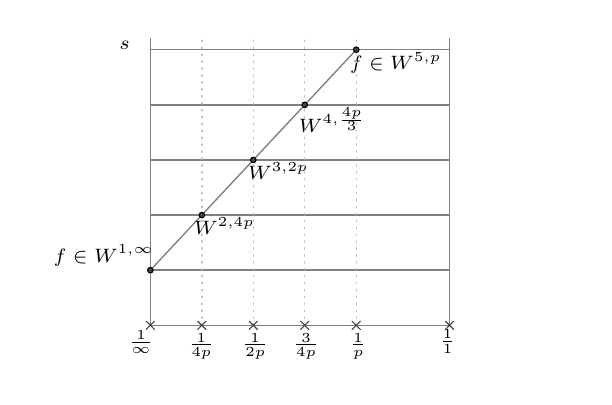
\begin{tikzpicture}[line cap=round,line join=round,>=triangle 45,x=3.8cm,y=0.7cm]
\clip(-0.41,-0.9277074696345513) rectangle (1.45,5.4);
%Quadricula
\draw [line width=.5pt,color=grisfosc] (0.,0.) -- (0.,5.203518980893238);
\draw [line width=.5pt,color=grisfosc] (1.,0.) -- (1.,5.203518980893238);
\draw [line width=.5pt,color=grisfosc] (0.,5.)-- (1.,5.);
\draw [line width=.5pt,color=grisfosc] (0.,3.)-- (1.,3.);
\draw [line width=.5pt,color=grisfosc] (0.,4.)-- (1.,4.);
\draw [line width=.5pt,color=grisfosc] (0.,2.)-- (1.,2.);
\draw [line width=.5pt,color=grisfosc] (0.,1.)-- (1.,1.);
\draw [line width=.5pt,color=grisfosc] (0.,0.)-- (1.,0.);
\begin{scriptsize}
\draw (-0.13,5.3) node[anchor=north west] {$s$};
\draw (0.94,0.057219536897733694) node[anchor=north west] {$\frac11$};
\draw (-0.1,0.05) node[anchor=north west] {$\frac1\infty$};
\end{scriptsize}
%Interpolation line
\draw [line width=.5pt,color=grisfosc] (0.6880985479597884,5.)-- (0.,1.);
\begin{scriptsize}
\draw (0.64,5.1) node[anchor=north west] {$f\in W^{5,p}$};
\draw (0.47,4.1) node[anchor=north west] {$W^{4,\frac{4p}3}$};
\draw (0.3,3.1) node[anchor=north west] {$W^{3,2p}$};
\draw (0.12,2.1) node[anchor=north west] {$W^{2,4p}$};
\draw (-0.35,1.6) node[anchor=north west] {$f\in W^{1,\infty}$};
\end{scriptsize}
%Vertical lines
\draw [line width=0.5pt,dotted,color=cqcqcq] (0.1720246369899471,0.) -- (0.1720246369899471,5.203518980893238);
\draw [line width=0.5pt,dotted,color=cqcqcq] (0.34404927397989427,0.) -- (0.34404927397989427,5.203518980893238);
\draw [line width=0.5pt,dotted,color=cqcqcq] (0.5160739109698413,0.) -- (0.5160739109698413,5.203518980893238);
\draw [line width=0.5pt,dotted,color=cqcqcq] (0.6880985479597884,0.) -- (0.6880985479597884,5.203518980893238);
\begin{scriptsize}
\draw (0.1,0) node[anchor=north west] {$\frac1{4p}$};
\draw (0.28,0) node[anchor=north west] {$\frac1{2p}$};
\draw (0.45,0) node[anchor=north west] {$\frac3{4p}$};
\draw (0.64,0) node[anchor=north west] {$\frac1{p}$};
\draw [fill=uuuuuu] (0.,1.) circle (1.0pt);
\draw [fill=uuuuuu] (0.6880985479597884,5.) circle (1.0pt);
\draw [fill=uuuuuu] (0.34404927397989427,3.) circle (1.0pt);
\draw [fill=uuuuuu] (0.1720246369899471,2.) circle (1.0pt);
\draw [color=uuuuuu] (0.,0.)-- ++(-1.5pt,-1.5pt) -- ++(3.0pt,3.0pt) ++(-3.0pt,0) -- ++(3.0pt,-3.0pt);
\draw [color=uuuuuu] (0.1720246369899471,0.)-- ++(-1.5pt,-1.5pt) -- ++(3.0pt,3.0pt) ++(-3.0pt,0) -- ++(3.0pt,-3.0pt);
\draw [color=uuuuuu] (0.34404927397989427,0.)-- ++(-1.5pt,-1.5pt) -- ++(3.0pt,3.0pt) ++(-3.0pt,0) -- ++(3.0pt,-3.0pt);
\draw [color=uuuuuu] (0.6880985479597884,0.)-- ++(-1.5pt,-1.5pt) -- ++(3.0pt,3.0pt) ++(-3.0pt,0) -- ++(3.0pt,-3.0pt);
\draw [fill=uuuuuu] (0.5160739109698413,4.) circle (1.0pt);
\draw [color=uuuuuu] (0.5160739109698413,0.)-- ++(-1.5pt,-1.5pt) -- ++(3.0pt,3.0pt) ++(-3.0pt,0) -- ++(3.0pt,-3.0pt);
\draw [color=uuuuuu] (1.,0.)-- ++(-1.5pt,-1.5pt) -- ++(3.0pt,3.0pt) ++(-3.0pt,0) -- ++(3.0pt,-3.0pt);
\end{scriptsize}
\end{tikzpicture}
\, 
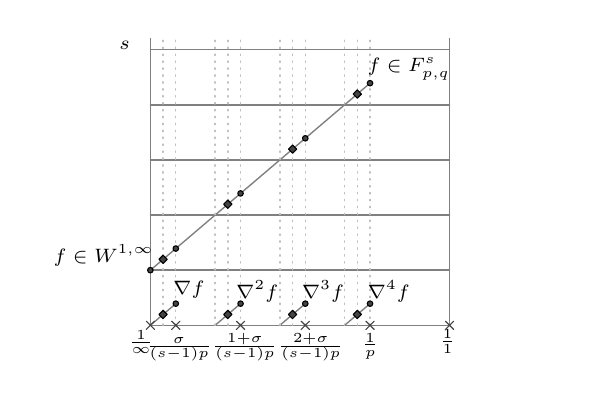
\begin{tikzpicture}[line cap=round,line join=round,>=triangle 45,x=3.8cm,y=0.7cm]
\clip(-0.41,-0.9277074696345513) rectangle (1.45,5.4);
%Quadricula
\draw [line width=.5pt,color=grisfosc] (0.,0.) -- (0.,5.203518980893238);
\draw [line width=.5pt,color=grisfosc] (1.,0.) -- (1.,5.203518980893238);
\draw [line width=.5pt,color=grisfosc] (0.,5.)-- (1.,5.);
\draw [line width=.5pt,color=grisfosc] (0.,3.)-- (1.,3.);
\draw [line width=.5pt,color=grisfosc] (0.,4.)-- (1.,4.);
\draw [line width=.5pt,color=grisfosc] (0.,2.)-- (1.,2.);
\draw [line width=.5pt,color=grisfosc] (0.,1.)-- (1.,1.);
\draw [line width=.5pt,color=grisfosc] (0.,0.)-- (1.,0.);
\begin{scriptsize}
\draw (-0.13,5.3) node[anchor=north west] {$s$};
\draw (0.94,0.057219536897733694) node[anchor=north west] {$\frac11$};
\draw (-0.1,0.05) node[anchor=north west] {$\frac1\infty$};
\end{scriptsize}
%Interpolation lines
\draw [line width=.5pt,color=grisfosc] (0.7341623110203971,4.392796751026526)-- (0.,1.);
\draw [line width=.5pt,color=grisfosc] (0.08499671264059261,0.392796751026526)-- (0.,0.);
\draw [line width=.5pt,color=grisfosc] (0.3013852454338608,0.392796751026526)-- (0.21638853279326817,0.);
\draw [line width=.5pt,color=grisfosc] (0.517773778227129,0.392796751026526)-- (0.4327770655865364,0.);
\draw [line width=.5pt,color=grisfosc] (0.7341623110203971,0.392796751026526)-- (0.6491655983798045,0.);
%Vertical lines0
\draw [line width=0.5pt,dotted,color=cqcqcq] (0.21638853279326817,0.) -- (0.21638853279326817,5.203518980893238);
\draw [line width=0.5pt,dotted,color=cqcqcq] (0.4327770655865364,0.) -- (0.4327770655865364,5.203518980893238);
\draw [line width=0.5pt,dotted,color=cqcqcq] (0.6491655983798045,0.) -- (0.6491655983798045,5.203518980893238);
\draw [line width=0.5pt,dotted,color=cqcqcq] (0.7341623110203971,0.) -- (0.7341623110203971,5.203518980893238);
\draw [line width=0.5pt,dotted,color=cqcqcq] (0.517773778227129,0.) -- (0.517773778227129,5.203518980893238);
\draw [line width=0.5pt,dotted,color=cqcqcq] (0.30138524543386075,0.) -- (0.30138524543386075,5.203518980893238);
\draw [line width=0.5pt,dotted,color=cqcqcq] (0.08499671264059261,0.) -- (0.08499671264059261,5.203518980893238);
\draw [line width=0.5pt,dotted,color=cqcqcq] (0.042498356320296304,0.) -- (0.042498356320296304,5.203518980893238);
\draw [line width=0.5pt,dotted,color=cqcqcq] (0.25888688911356444,0.) -- (0.25888688911356444,5.203518980893238);
\draw [line width=0.5pt,dotted,color=cqcqcq] (0.4752754219068327,0.) -- (0.4752754219068327,5.203518980893238);
\draw [line width=0.5pt,dotted,color=cqcqcq] (0.6916639547001008,0.) -- (0.6916639547001008,5.203518980893238);
\begin{scriptsize}
\draw (0.7,5) node[anchor=north west] {$f\in F^s_{p,q}$};
\draw (-0.35,1.6) node[anchor=north west] {$f\in W^{1,\infty}$};
\draw (-0.04,-0.08) node[anchor=north west] {$\frac{\sigma}{(s-1)p}$};
\draw (0.18,0) node[anchor=north west] {$\frac{1+\sigma}{(s-1)p}$};
\draw (0.4,0) node[anchor=north west] {$\frac{2+\sigma}{(s-1)p}$};
\draw (0.68,0) node[anchor=north west] {$\frac1{p}$};
\draw (0.7,0.95) node[anchor=north west] {$\nabla^4 f$};
\draw (0.48,0.95) node[anchor=north west] {$\nabla^3 f$};
\draw (0.26,0.95) node[anchor=north west] {$\nabla^2 f$};
\draw (0.05,0.95) node[anchor=north west] {$\nabla f$};
%cercles
\draw [fill=uuuuuu] (0.,1.) circle (1.0pt);
\draw [fill=uuuuuu] (0.7341623110203971,4.392796751026526) circle (1.0pt);
\draw [fill=uuuuuu] (0.7341623110203971,0.392796751026526) circle (1.0pt);
\draw [fill=uuuuuu] (0.517773778227129,0.392796751026526) circle (1.0pt);
\draw [fill=uuuuuu] (0.3013852454338608,0.392796751026526) circle (1.0pt);
\draw [fill=uuuuuu] (0.08499671264059261,0.392796751026526) circle (1.0pt);
\draw [fill=uuuuuu] (0.517773778227129,3.3927967510265256) circle (1.0pt);
\draw [fill=uuuuuu] (0.3013852454338608,2.392796751026526) circle (1.0pt);
\draw [fill=uuuuuu] (0.08499671264059261,1.392796751026526) circle (1.0pt);
%quadrats
\draw [fill=uuuuuu] (0.2588868891135645,0.196398375513263)  ++(-1.5pt,0 pt) -- ++(1.5pt,1.5pt)--++(1.5pt,-1.5pt)--++(-1.5pt,-1.5pt)--++(-1.5pt,1.5pt);
\draw [fill=uuuuuu] (0.4752754219068327,0.196398375513263)  ++(-1.5pt,0 pt) -- ++(1.5pt,1.5pt)--++(1.5pt,-1.5pt)--++(-1.5pt,-1.5pt)--++(-1.5pt,1.5pt);
\draw [fill=uuuuuu] (0.6916639547001008,0.196398375513263)  ++(-1.5pt,0 pt) -- ++(1.5pt,1.5pt)--++(1.5pt,-1.5pt)--++(-1.5pt,-1.5pt)--++(-1.5pt,1.5pt);
\draw [fill=uuuuuu] (0.4752754219068327,3.1963983755132626)  ++(-1.5pt,0 pt) -- ++(1.5pt,1.5pt)--++(1.5pt,-1.5pt)--++(-1.5pt,-1.5pt)--++(-1.5pt,1.5pt);
\draw [fill=uuuuuu] (0.2588868891135645,2.196398375513263)  ++(-1.5pt,0 pt) -- ++(1.5pt,1.5pt)--++(1.5pt,-1.5pt)--++(-1.5pt,-1.5pt)--++(-1.5pt,1.5pt);
\draw [fill=uuuuuu] (0.042498356320296304,1.196398375513263)  ++(-1.5pt,0 pt) -- ++(1.5pt,1.5pt)--++(1.5pt,-1.5pt)--++(-1.5pt,-1.5pt)--++(-1.5pt,1.5pt);
\draw [fill=uuuuuu] (0.6916639547001008,4.1963983755132634)  ++(-1.5pt,0 pt) -- ++(1.5pt,1.5pt)--++(1.5pt,-1.5pt)--++(-1.5pt,-1.5pt)--++(-1.5pt,1.5pt);
\draw [fill=uuuuuu] (0.042498356320296304,0.196398375513263) ++(-1.5pt,0 pt) -- ++(1.5pt,1.5pt)--++(1.5pt,-1.5pt)--++(-1.5pt,-1.5pt)--++(-1.5pt,1.5pt);
%Creus
\draw [color=uuuuuu] (0.,0.)-- ++(-1.5pt,-1.5pt) -- ++(3.0pt,3.0pt) ++(-3.0pt,0) -- ++(3.0pt,-3.0pt);
%\draw [color=uuuuuu] (0.21638853279326817,0.)-- ++(-1.5pt,-1.5pt) -- ++(3.0pt,3.0pt) ++(-3.0pt,0) -- ++(3.0pt,-3.0pt);
%\draw [color=uuuuuu] (0.4327770655865364,0.)-- ++(-1.5pt,-1.5pt) -- ++(3.0pt,3.0pt) ++(-3.0pt,0) -- ++(3.0pt,-3.0pt);
\draw [color=uuuuuu] (0.7341623110203971,0.)-- ++(-1.5pt,-1.5pt) -- ++(3.0pt,3.0pt) ++(-3.0pt,0) -- ++(3.0pt,-3.0pt);
%\draw [color=uuuuuu] (0.6491655983798045,0.)-- ++(-1.5pt,-1.5pt) -- ++(3.0pt,3.0pt) ++(-3.0pt,0) -- ++(3.0pt,-3.0pt);
\draw [color=uuuuuu] (0.517773778227129,0.)-- ++(-1.5pt,-1.5pt) -- ++(3.0pt,3.0pt) ++(-3.0pt,0) -- ++(3.0pt,-3.0pt);
\draw [color=uuuuuu] (0.30138524543386075,0.)-- ++(-1.5pt,-1.5pt) -- ++(3.0pt,3.0pt) ++(-3.0pt,0) -- ++(3.0pt,-3.0pt);
\draw [color=uuuuuu] (0.08499671264059261,0.)-- ++(-1.5pt,-1.5pt) -- ++(3.0pt,3.0pt) ++(-3.0pt,0) -- ++(3.0pt,-3.0pt);
\draw [color=uuuuuu] (1,0.)-- ++(-1.5pt,-1.5pt) -- ++(3.0pt,3.0pt) ++(-3.0pt,0) -- ++(3.0pt,-3.0pt);
%\draw [color=uuuuuu] (0.042498356320296304,0.)-- ++(-1.5pt,-1.5pt) -- ++(3.0pt,3.0pt) ++(-3.0pt,0) -- ++(3.0pt,-3.0pt);
%\draw [color=uuuuuu] (0.25888688911356444,0.)-- ++(-1.5pt,-1.5pt) -- ++(3.0pt,3.0pt) ++(-3.0pt,0) -- ++(3.0pt,-3.0pt);
%\draw [color=uuuuuu] (0.4752754219068327,0.)-- ++(-1.5pt,-1.5pt) -- ++(3.0pt,3.0pt) ++(-3.0pt,0) -- ++(3.0pt,-3.0pt);
%\draw [color=uuuuuu] (0.6916639547001008,0.)-- ++(-1.5pt,-1.5pt) -- ++(3.0pt,3.0pt) ++(-3.0pt,0) -- ++(3.0pt,-3.0pt);
\end{scriptsize}
\end{tikzpicture}
\end{figure}


According to the previous result,  we will prove some properties  for subspaces of $W^{s,p}$ whose functions have bounded first derivatives. Namely, we define the space $\mathbf{W}^{s,p}(\Omega):=W^{s,p}(\Omega)\cap C^{0,1}(\Omega)$. By the Sobolev embedding Theorem, when $sp>d$ we have that $\mathbf{W}^{s+1,p}(\Omega)=W^{s+1,p}(\Omega)$.




\begin{lemma}\label{lemSobolevAdmissibleSpace}
Let $s,d\in\N$, and $ 1< p< \infty$. Given bounded Lipschitz domains $\Omega_j\subset \R^d$ and functions $f,g$ with $f(\Omega_1)= \Omega_2$ and $f$ bi-Lipzchitz, then 
\begin{align}\label{eqInvarianceUnderbiLipschitzSOBOBis}
f \in \mathbf{W}^{s,p}(\Omega_1) \mbox{ and } g \in \mathbf{W}^{s,p}(\Omega_2) & \implies g \circ f \in {W}^{s,p}(\Omega_1),\\
\nonumber f \in \mathbf{W}^{s,\frac{ps}{s-1}}(\Omega_1)\mbox{ and } g \in {W}^{s,p}\cap L^\infty(\Omega_1) & \implies   g \circ f \in {W}^{s,p}(\Omega_1)
\end{align}
(see Figure \ref{figComposition}) and the chain rule \rf{eqGeneralizedChainRule} applies (for $M=s$). Moreover,
\begin{equation}\label{eqInvarianceUnderInversionSOBOBis}
f \in \mathbf{W}^{s,p}(\Omega_1)  \implies f^{-1} \in {W}^{s,p}(\Omega_2),
\end{equation}
and \rf{eqDerivativesInverse} holds.
\end{lemma}


\begin{proof}
To check \rf{eqInvarianceUnderbiLipschitzSOBOBis}, the case $s=1$ is \cite[Theorem 2.2.2]{Ziemer}, so let us assume that $s\geq 2$.  Since both $f_1$ and $f_2$ are in $ W^{s,p}(\Omega_j)$, all their derivatives satisfy that $\nabla^i f_j\in L^{p\frac{s-1}{i-1}}$ in view of Lemma \ref{lemReadyForHolderInequality}. 

By Remark \ref{remChainRule}, we only need to check that the right-hand side of \rf{eqGeneralizedChainRule} is in $L^p$, and then by induction it follows that the chain rule applies. By H\"older's inequality, 
\begin{equation}\label{eqCompositionDecomposition}
\circled{1}:=\norm{\sum_{1\leq i\leq s} \sum_{\alpha\in\N^i: |\alpha|=s}   \nabla^i f_2(f_1) \prod_{\ell=1}^{i} \nabla^{\alpha_\ell}f_1}_{L^p} \lesssim_{d,s}  \sum_{1\leq i\leq s} \sum_{\alpha\in\N^i: |\alpha|=s}   \norm{\nabla^i f_2(f_1)}_{p_0} \prod_{\ell=1}^{i} \norm{\nabla^{\alpha_\ell}f_1}_{p_\ell},
\end{equation}
where $\sum_0^i \frac{1}{p_\ell}=\frac1p$. This can be achieved by letting ${p_0}=\frac{p(s-1)}{i-1}$ and ${p_\ell}=\frac{p(s-1)}{\alpha_\ell-1}$. Thus,  Lemma \ref{lemReadyForHolderInequality} applies and using Young's inequality for products  we get 
\begin{align}\label{eqGeneralizedChainRuleSobolev}
\circled{1}
	& \lesssim \sum_i \norm{\nabla f_1^{-1}}_{\infty}^{\frac{d(i-1)}{p(s-1)}}  \norm{f_2}_{ W^{s,p}(\Omega_2)}^{\frac{i-1}{s-1}}\norm{\nabla f_2}_{L^\infty(\Omega_2)}^{\frac{s-i}{s-1}}  \norm{f_1}_{ W^{s,p}(\Omega_1)}^{\frac{s-i}{s-1}}\norm{\nabla f_1}_{ L^\infty(\Omega_1)}^{\frac{is-s}{s-1}}\\
	\nonumber & \lesssim C_{f_1}   (\norm{f_2}_{{W}^{s,p}(\Omega_2)}\norm{\nabla f_1}_{L^\infty(\Omega_1)}^s+\norm{\nabla f_2}_{L^\infty(\Omega_2)}\norm{f_1}_{{W}^{s,p}(\Omega_1)}),
\end{align}
with the constant $C_{f_1}$ depending on the bi-Lipschitz character of $f_1$.

%
%Consider now general functions $f_j\in \mathbf{W}^{s,p}(\Omega_j)$ with $f_1$ bi-Lipschitz. Let $\Lambda_{\Omega_j}$ be an extension operator for $\mathbf{W}^{s,p}(\Omega_j)$ (see \cite[Theorem VI.5]{SteinPetit}). Consider approximations of the identity $f_j^\varepsilon=\Lambda_{\Omega_j} f_j * \varphi_\varepsilon$ for a $C^\infty_c$ function $\varphi$ with $\int\varphi=1$. 
%
%Clearly $f_j^\varepsilon\to f_j$ in ${W}^{s,p}(\Omega_j)$ and the first order derivatives of $f_j^\varepsilon$ converge uniformly to the corresponding derivatives of $f_j$. Thus, the bi-Lipschitz character is preserved for $\varepsilon$ small enough and estimate \rf{eqGeneralizedChainRuleSobolev} holds uniformly, extending to the limiting case  via Banach-Alaoglu Theorem.

The second inclusion in \rf{eqInvarianceUnderbiLipschitzSOBOBis} can be shown analogously, setting ${p_0}=\frac{ps}{i}$ and ${p_\ell}=\frac{ps}{\alpha_\ell-1}$ in \rf{eqCompositionDecomposition}.  We leave the details to the reader.

The inverse function bound \rf{eqInvarianceUnderInversionSOBOBis} can be proven by the same methods using \rf{eqDerivativesInverse}. 
Indeed, \rf{eqInverseDerivatives} holds for every bi-Lipschitz function by the chain rule, and arguing as in Remark \ref{remChainRule}, we only need to check that the right-hand side in \rf{eqDerivativesInverse}  belongs to $L^p$ for every $|\alpha|=s$ in order to prove that \rf{eqDerivativesInverse} holds and that $g_{ij}\in W^{s-1,p}(\Omega_1)$. Indeed, 
\begin{align*}
& \norm{\sum_{ \substack{ \gamma\in(\N_0^d)^{s-1}\\ |\gamma_\ell|\geq 1\, \&\,\sum|\gamma_\ell|=2s-2}} |D f|^{(d-1)s} \prod_{\ell=1}^{s-1} |D^{\gamma_\ell} f| |D(f^{-1})|^{ds}}_{L^p} \\
	& \quad \lesssim_{d,s}   \sum_{ \substack{ \gamma\in(\N_0^d)^{s-1}\\ |\gamma_\ell|\geq 1\, \&\,\sum|\gamma_\ell|=2s-2}} \norm{D f}_\infty^{(d-1)s} \prod_{\ell=1}^{s-1} \norm{D^{\gamma_\ell} f}_{p_\ell}\norm{D(f^{-1})}_{L^\infty(\Omega)}^{ds}\\
	&\quad  \lesssim \norm{f}_{W^{s,p}(\Omega)}\norm{Df}_{L^\infty(\Omega)}^{ds-2}\norm{D(f^{-1})}_{L^\infty(\Omega)}^{ds}
\end{align*}
by choosing ${p_\ell}=\frac{p(s-1)}{|\gamma_\ell|-1}$ and applying Lemma \ref{lemReadyForHolderInequality} with $q=2$. We obtain that $g_{ij}\in W^{s-1,p}(\Omega_1)$ and \rf{eqDerivativesInverse} holds. 

On the other hand, if $s=2$ then $f\in C^{0,1}$ and $f^{-1}\in C^{0,1}$. By \rf{eqInverseDerivatives} and \rf{eqInvarianceUnderbiLipschitzSOBOBis} we get $(D(f^{-1}))_{ij}\in W^{s-1,p}(\Omega_2)$.
If, instead, $s>2$ then $f\in \mathbf{W}^{s-1,\frac{p(s-1)}{s-2}}(\Omega_1)$  by Lemma \ref{lemReadyForHolderInequality} and therefore, by induction, we can assume that \rf{eqInvarianceUnderInversionSOBOBis} holds in this case, so  $f^{-1} \in W^{s-1,\frac{p(s-1)}{s-2}}(\Omega_2)$ and applying the second estimate in \rf{eqInvarianceUnderbiLipschitzSOBOBis} to the composition in \rf{eqInverseDerivatives} we get that $(D(f^{-1}))_{ij}\in W^{s-1,p}(\Omega_2)$. 
\end{proof}



%\Marti{MISSING: If we only assumed that the functions are $W^{1,\infty}$ instead of $C^1$, then the approximations would not be necessarily bi-Lipschitz. Is that correct? We may consider the following alternative approach in the spirit of \cite[2.2.2]{Ziemer}: Instead of approximating both $f_1$ and $f_2$, approximate only $f_2$ and keep $f_1$ fixed. Then, Faa di Bruno is satisfied at the differentiability points of $f_2^\varepsilon\circ f_1$, which are the differentiability points of $f_1$. Is that true? Is that enough? Does this allow us to switch the rather artificial $C^1$ condition for $W^{1,\infty}$?}



\subsection{Proof or Theorem \ref{theoTriebelAdmissibleBanachBis}: the Triebel-Lizorkin scale}
Finally we will verify that Triebel-Lizorkin spaces have the same properties.
%, proving Lemma \ref{lemTriebelAdmissibleBanach},  Lemma \ref{lemBesovAdmissibleSpace} being a particular case. 
Again, we define $\mathbf{F}^s_{p,q}(\Omega):=F^{s}_{p,q}(\Omega) \cap C^{0,1}(\Omega)$ for $k<s<k+1$. Note that when $sp>d$ we have that $\mathbf{F}^{s+1}_{p,q}(\Omega)=F^{s+1}_{p,q}(\Omega)$.

%
%\begin{lemma}\label{lemReadyForHolderInequality}
%Let ${k} \in \N_0$, $0<\sigma \leq 1$ and  $s:={k}+\sigma$, let $ 1\leq p < \infty$, $ 1\leq q \leq\infty$ and $d\in\N$ and let $f\in F^{s}_{p,q}(\Omega)\cap W^{1,\infty}(\Omega)$ where $\Omega\subset\R^d$ is a Lipschitz domain. Then, for every positive index $j\leq k$
%$$\norm{\nabla^j f}_{ L^{p\frac{s-1}{j-1}}(\Omega)}\lesssim_{s,p,q,j,\Omega}  \norm{f}_{ F^{s}_{p,q}(\Omega)}^{\frac{j-1}{s-1}}\norm{\nabla f}_{ L^\infty(\Omega)}^{\frac{s-j}{s-1}} .$$
%Moreover, for every $1\leq r\leq \infty$ and $M\geq 1$ with $j+\sigma/M<s$, we have
%$$\norm{\nabla^j f}_{ F^{\sigma/M}_{\frac{p(s-1)}{j+\sigma/M-1},r}(\Omega)}\lesssim_{s,p,q,r,j+\sigma/M,\Omega} \norm{f}_{F^{s}_{p,q}(\Omega)}^{\frac{j+\sigma/M-1}{s-1}} \norm{\nabla f}_{ L^\infty(\Omega)}^{\frac{s-j-\sigma/M}{s-1}} .$$
%\end{lemma}
%Note that $j+\sigma/M<s$ excludes only the case when both $M=1$ and $j=k$.








\begin{proof}[Proof of \rf{eqInvarianceUnderbiLipschitzTRIEBELBis}]
Let us write $\Omega=\Omega_1$. We begin by showing \rf{eqInvarianceUnderbiLipschitzTRIEBELBis}. Since the case ${k}=0$ follows from Theorem \ref{theoDifference}, we assume $ k \geq 1$. Also by Theorem \ref{theoDifference}, it is enough to check that 
\begin{equation}\label{eqQuantifyComposition}
\circled{1}:=\int_\Omega \left(\int_0^1 \frac{\left( \int_{B(x,t)\cap\Omega} |\nabla^k (g\circ f)(x)-\nabla^k (g\circ f)(y)| dy\right)^q}{t^{(\sigma+d)q}}\frac{dt}{t} \right)^\frac pq dx  \leq C_{f}^p\norm{g}_{\mathbf{F}^{s}_{p,q}(\Omega_2)}^p.
\end{equation}

By Lemma \ref{lemSobolevAdmissibleSpace} we can use the chain rule 
almost everywhere and in particular \rf{eqGeneralizedChainRuleDifferences} applies.  However, after considering \rf{eqGeneralizedChainRuleDifferences}, the reader will note that there are functions on $x$ and functions on $y$ in the integrand, and this is an obstruction for using H\"older inequalities as it was done in the previous proof. Instead, we need to write all the functions depending on $x$ and then address all the terms appearing in a telescopic summation. To keep the notation compact, we write $\Delta_h g(x):=g(x+h)-g(x)$ for $h=y-x$ in \rf{eqGeneralizedChainRuleDifferences}. It follows that $\Delta_h(g_1g_2)=\Delta_h g_1\Delta_hg_2+\Delta_h g_1 g_2+g_1\Delta_hg_2$ and, by induction, 





\begin{equation}\label{eqDifferencesProduct}
\prod_{i=1}^\ell g_i (x+h) =  \sum_{\nu \in \{0,1\}^{\ell}} \prod_{r\leq \ell: \nu_r=1} \Delta_h g_r (x)  \prod_{e\leq \ell: \nu_e=0} g_e(x).
\end{equation} 
Combining with \rf{eqGeneralizedChainRuleDifferences}  we get
\begin{align}\label{eqGeneralizedChainRuleDifferencesLonger}
 |\Delta_h &\nabla^k (g\circ f) (x)|\\
\nonumber	& \lesssim  \sum_{1\leq i\leq k} |\Delta_h [( \nabla^{i} g)\circ f](x)| \sum_{\alpha\in\N^i: |\alpha|=k} \prod_{j=1}^{i} | \nabla^{\alpha_j} f (x)| \\
\nonumber	&  + \sum_{1\leq i\leq k} | \nabla^i g(f(x))| \sum_{\substack{\alpha\in\N^i\\ |\alpha|=k} } \sum_{\ell=1}^{i} \sum_{\substack{\nu \in \{0,1\}^{i} \\ \nu_\ell=1 \\ \nu_r=0   \,\forall r>\ell}} \prod_{r\leq i: \nu_r=1}|\Delta_h (\nabla^{\alpha_r} f) (x) | \prod_{e\leq i: \nu_e=0}
|\nabla^{\alpha_e} f (x)|\\
\nonumber	&  + \sum_{1\leq i\leq k} |\Delta_h [( \nabla^{i} g)\circ f](x)|  \sum_{\substack{\alpha\in\N^i\\ |\alpha|=k} } \sum_{\ell=1}^{i} \sum_{\substack{\nu \in \{0,1\}^{i} \\ \nu_\ell=1 \\ \nu_r=0 \,\forall r>\ell}} \prod_{r\leq i: \nu_r=1}|\Delta_h (\nabla^{\alpha_r} f) (x) | \prod_{e\leq i: \nu_e=0}|\nabla^{\alpha_e} f (x)|.
\end{align}
 

Plugging this decomposition in the numerator of the integrand in \rf{eqQuantifyComposition}, we get 
 \begin{align}\label{eqBreakTheBesovNormOfComposition}
\circled{1}
	& \lesssim \sum_{1\leq i\leq k}\sum_{\substack{\alpha\in\N^i\\ |\alpha|=k} }  \squared{$2i\alpha$}+ \sum_{1\leq i\leq k} \sum_{\substack{\alpha\in\N^i\\ |\alpha|=k} } \sum_{\ell=1}^{i} \sum_{\substack{\nu \in \{0,1\}^{i} \\ \nu_\ell=1 \\ \nu_r=0   \,\forall r>\ell}} \left(\squared{$3i\alpha\ell\nu$}+\squared{$4i\alpha\ell\nu$}\right),
\end{align}
and the coefficients $\alpha_j$ are all strictly positive natural numbers.
Regarding the first term, we have
\begin{align*}
\squared{$2i\alpha$} 
	& = \int_\Omega \left(\int_0^1 \frac{ \left( \int_{(B(x,t)\cap\Omega)-x} |\Delta_h [( \nabla^{i} g)\circ f](x)| dh\right)^q }{t^{(\sigma+d)q}}\frac{dt}{t} \right)^\frac pq \prod_{j=1}^{i} | \nabla^{\alpha_j} f (x)|^p dx \\
	& \lesssim \norm{\nabla f^{-1}}_\infty^{\frac {dp}{p_0}+ {dp}} \norm{\nabla f}_\infty^{\left(\sigma+d\right)p} \norm{\nabla^{i} g}_{F^{\sigma}_{p_{0},q}(\Omega_2)}^p \prod_{j=1}^{i} \norm{\nabla^{\alpha_j}  f}_{L^{p_{j}}(\Omega_1)}^p,
\end{align*}
where $\sum_0^i \frac{1}{p_{j}}=\frac1p$. Note that we have used $f$ as a bi-Lipschitz change of variables to obtain the $F^\sigma_{p_0,q}$ norm in the right-hand side of the last inequality above. Letting ${p_0}=\frac{p(s-1)}{i+\sigma-1}$ and ${p_j}=\frac{p(s-1)}{\alpha_j-1}$ so that we can apply Lemma \ref{lemReadyForHolderInequality}, and noting that $\sum_1^i  \alpha_j-1=k-i$ and $\sum_1^i s-\alpha_j=i s-k$, we get
\begin{align*}
\squared{$2i\alpha$}^\frac1p
	& \lesssim \norm{\nabla f^{-1}}_\infty^{\frac d{p_0}+d} \norm{\nabla f}_\infty^{d}  \norm{g}_{F^{s}_{p,q}(\Omega_2)}^\frac{i+\sigma-1}{s-1}\norm{\nabla g}_\infty^\frac{s-i-\sigma}{s-1} \norm{f}_{F^{s}_{p,q}(\Omega_1)}^{\sum_1^i  \frac{\alpha_j-1}{s-1}} \norm{\nabla f}_\infty^{\sigma + \sum_1^i \frac{s-\alpha_j}{s-1}}\\
	&= C_{f}  \left(\norm{g}_{F^{s}_{p,q}(\Omega_2)}\norm{\nabla f}_\infty^{s}\right)^\frac{i+\sigma-1}{s-1}\left(\norm{\nabla g}_\infty\norm{f}_{F^{s}_{p,q}(\Omega_1)}\right)^\frac{k-i}{s-1} \\
	&\leq C_{f} \left( \norm{g}_{F^{s}_{p,q}(\Omega_2)}\norm{\nabla f}_\infty^{s} + \norm{\nabla g}_\infty\norm{f}_{F^{s}_{p,q}(\Omega_1)}\right),
\end{align*}
where $C_{f}=\norm{\nabla f^{-1}}_\infty^{\frac d{p_0}+d} \norm{\nabla f}_\infty^{d} $ depends only on the bi-Lipschitz character of $f$.

For the second term in the right-hand side of \rf{eqBreakTheBesovNormOfComposition}, we need to apply H\"older inequality three times, once for each variable. Namely, writing $U_{x}^t:=B(x,t)\cap\Omega-x$, 
\begin{align*}
\squared{$3i\alpha\ell\nu$} 
	& = \int_\Omega \left(\int_0^1  \frac{\left( \int_{U_{x}^t}\prod_{r\leq i: \nu_r=1}|\Delta_h (\nabla^{\alpha_r} f) (x) | dh\right)^q}{t^{(\sigma+d)q}} \frac{dt}{t}\right)^\frac pq | \nabla^i g(f(x))|^p \prod_{e\leq i: \nu_e=0} |\nabla^{\alpha_e} f (x)|^p dx\\
	& \leq \int_\Omega \prod_{r\leq i: \nu_r=1} \left(\int_0^1  \frac{\left( \int_{U_{x}^t}|\Delta_h (\nabla^{\alpha_r} f) (x) |^{u_r} dh\right)^\frac{q_r}{u_r} }{t^{(\sigma+d)q}} \frac{dt}{t}\right)^\frac {p}{q_r} | \nabla^i g(f(x))|^p \prod_{e\leq i: \nu_e=0} |\nabla^{\alpha_e} f (x)|^p dx
\end{align*}
where we assume that $\sum_r \frac1{u_r}=\sum_r \frac q{q_r}=1$. In particular, let us fix $q_r:=u_r q$ so that  $(\sigma+d)q=(\frac{\sigma q}{q_r}+\frac{d}{u_r})q_r$. Take also $\sum_0^i \frac{1}{p_{j}}=\frac1p$ and apply H\"older's inequality again to get
\begin{align*}
\squared{$3i\alpha\ell\nu$} 
	& \lesssim \norm{\nabla f^{-1}}_\infty^{\frac {dp}{p_0}} \norm{\nabla^i g}_{L^{p_{0}}(\Omega_2)}^p \prod_{r\leq i: \nu_r=1} \norm{\nabla^{\alpha_r} f}_{F^{\sigma q/q_r}_{p_r,q_r}(\Omega_1)}^p \prod_{e\leq i: \nu_e=0} \norm{\nabla^{\alpha_e} f }_{L^{p_{e}}(\Omega_1)}^p, 
\end{align*}
as long as $1\leq u_r\leq \min\{p_r,q_r\} \frac{d+\sigma}{d}$. 

The fact that $u_r\leq q_r$ is clear from the definition of $q_r$. 
Let us write $M=\sum_{r:\nu_r=1}(\alpha_r-1)$ and define $u_r:= \frac{M}{\alpha_r - 1}$, $p_0:= \frac{p(s-1)}{i-1}$, $p_r=\frac{p(s-1)}{\alpha_r+\sigma/u_r -1}$ and $p_e=\frac{p(s-1)}{\alpha_e-1}$. Note that $\sum \frac1{u_r}=1$ and  $1\leq u_r$ trivially, while the condition $u_r \leq p_r$ is equivalent to $u_r(\alpha_r-1)\leq p(s-1) -\sigma$, that is, equivalent to $M\leq p(s-1) -\sigma$. But $M\leq |\alpha|-1= k-1=s-1-\sigma\leq p(s-1) -\sigma$, and thus it follows that $u_r\leq p_r$.

Thus, we can apply Lemma \ref{lemReadyForHolderInequality} again to get
\begin{align*}
\squared{$3i\alpha\ell\nu$}^\frac1p
	& \lesssim C_{f} \norm{g}_{F^{s}_{p,q}(\Omega_2)}^\frac{i-1}{s-1}\norm{\nabla g}_\infty^\frac{s-i}{s-1} \norm{f}_{F^{s}_{p,q}(\Omega_1)}^{\sum_r  \frac{\alpha_r+\sigma/u_r-1}{s-1}+\sum_e  \frac{\alpha_e-1}{s-1}} \norm{\nabla f}_\infty^{ \sum_r \frac{s-\alpha_r-\sigma/u_r}{s-1}+\sum_e \frac{s-\alpha_e}{s-1}}\\
	& \leq C_{f} \left( \norm{g}_{F^{s}_{p,q}(\Omega_2)}\norm{\nabla f}_\infty^{s} + \norm{\nabla g}_\infty\norm{f}_{F^{s}_{p,q}(\Omega_1)}\right),
\end{align*}
where $C_{f}= \norm{\nabla f^{-1}}_\infty^{\frac d{p_0}} $ depends only on the bi-Lipschitz character of $f$.


For the last term in the right-hand side of \rf{eqGeneralizedChainRuleDifferencesLonger}, we argue analogously to get
\begin{align*}
\squared{$4i\alpha\ell\nu$} 
	& =  \int_\Omega \left(\int_0^1  \frac{\left( \int_{U_{x}^t} |\Delta_h [( \nabla^{i} g)\circ f](x)| \prod_{\substack{r\leq i\\ \nu_r=1}}|\Delta_h (\nabla^{\alpha_r} f) (x) | dh\right)^q}{t^{(\sigma+d)q}} \frac{dt}{t}\right)^\frac pq  \prod_{\substack{e\leq i\\ \nu_e=0}} |\nabla^{\alpha_e} f (x)|^p dx\\
	& \leq  \int_\Omega \left(\int_0^1  \frac{\left( \int_{U_{x}^t} |\Delta_h [( \nabla^{i} g)\circ f](x)|^{u_0} dh\right)^\frac{q_0}{u_0}}{t^{(\sigma+d)q}} \frac{dt}{t}\right)^\frac p{q_0} \\
	&\quad  \cdot\left(\int_0^1  \frac{\left( \int_{U_{x}^t}\prod_{\substack{r\leq i\\ \nu_r=1}}|\Delta_h (\nabla^{\alpha_r} f) (x) |^{u_r} dh\right)^\frac{q_r}{u_r}}{t^{(\sigma+d)q}} \frac{dt}{t}\right)^\frac p{q_r}  \prod_{\substack{e\leq i\\ \nu_e=0}} |\nabla^{\alpha_e} f (x)|^p dx,
\end{align*}
where we assume
$\frac1{u_0}+\sum_r \frac1{u_r}=\frac{q}{q_0}+\sum_r \frac q{q_r}=1$. In particular, let us fix $q_0:=u_0 q$ and $q_r:=u_r q$ so that $(\sigma+d)q=(\frac{\sigma q}{q_r}+\frac{d}{u_r})q_r$. Take also $\sum_0^i \frac{1}{p_{j}}=\frac1p$ and apply H\"older's inequality again to get
\begin{align*}
\squared{$4i\alpha\ell\nu$} 
	& \lesssim \norm{\nabla f^{-1}}_\infty^{\frac {dp}{p_0}+\frac {dp}{u_0}} \norm{\nabla f}_\infty^{\frac{(\sigma +d) p}{u_0}} \norm{\nabla^i g}_{F^{\sigma q/q_0}_{p_0,q_0}(\Omega_2)}^p \prod_{\substack{r\leq i\\ \nu_r=1}} \norm{\nabla^{\alpha_r} f}_{F^{\sigma q/q_r}_{p_r,q_r}(\Omega_1)}^p \prod_{\substack{e\leq i\\ \nu_e=0}} \norm{\nabla^{\alpha_e} f }_{L^{p_{e}}(\Omega_1)}^p, 
\end{align*}
as long as $1\leq u_r\leq \min\{p_r,q_r\}  \frac{d+\sigma}{d}$. 

The fact that $u_r\leq q_r$ is clear from the definition of $q_r$. 
Let us write $M=\sum_r(\alpha_r-1)$ and define $u_0:=\frac{M+i-1}{i-1}$, $u_r:= \frac{M+i-1}{\alpha_r - 1}$, $p_0:= \frac{p(s-1)}{i+\sigma/u_0-1}$, $p_r=\frac{p(s-1)}{\alpha_r+\sigma/u_r -1}$ and $p_e=\frac{p(s-1)}{\alpha_e-1}$. Note that $\sum \frac1{u_r}=1$ and  $1\leq u_r$ trivially, while the condition $u_r \leq p_r$ is equivalent to $M+i-1\leq p(s-1) -\sigma$. But 
$$M+i-1\leq \sum_{j=1}^i(\alpha_j-1)+i-1= |\alpha|-1= k-1=s-1-\sigma\leq p(s-1) -\sigma,$$ and thus it follows that $u_r\leq p_r$.

Thus, we can apply Lemma \ref{lemReadyForHolderInequality} again to get
\begin{align*}
\squared{$4i\alpha\ell\nu$}^\frac1p
	& \lesssim C_{f} \norm{g}_{F^{s}_{p,q}(\Omega_2)}^\frac{i+\sigma/u_0-1}{s-1}\norm{\nabla g}_\infty^\frac{s-i-\sigma/u_0}{s-1} \norm{f}_{F^{s}_{p,q}(\Omega_1)}^{\sum_r  \frac{\alpha_r+\sigma/u_r-1}{s-1}+\sum_e  \frac{\alpha_e-1}{s-1}} \norm{\nabla f}_\infty^{ \frac\sigma {u_0}+\sum_r \frac{s-\alpha_r-\sigma/u_r}{s-1}+\sum_e \frac{s-\alpha_e}{s-1}}\\
	& \leq C_{f} \left( \norm{g}_{F^{s}_{p,q}(\Omega_2)}\norm{\nabla f}_\infty^{s} + \norm{\nabla g}_\infty\norm{f}_{F^{s}_{p,q}(\Omega_1)}\right),
\end{align*}
where $C_{f}=\norm{\nabla f^{-1}}_\infty^{\frac d{p_0}+\frac d{u_0}}  \norm{\nabla f}_\infty^{\frac {d}{u_0}}$ depends only on the bi-Lipschitz character of $f$.


Combining these estimates with \rf{eqBreakTheBesovNormOfComposition}, we obtain \rf{eqInvarianceUnderbiLipschitzTRIEBELBis}. In particular, we obtain \rf{eqQuantifyComposition}, where the constant $C_{f}$ is affine with respect to the  $F^{s}_{p,q}(\Omega)$ norm of $f$ and depends polynomially on its bi-Lipschitz constants, as well as on $d$, $s$, $p$, $q$ and the extension constants of the domains for all the different indices $p_j,q_j,u_j$ appearing in the proof.  
\end{proof}




\begin{figure}[t]
\caption{Composition rule for Sobolev and Triebel-Lizorkin scales of a bounded continuous function $g$ and a bi-Lipschitz function $f$ in Lemmas \ref{lemSobolevAdmissibleSpace} and \ref{theoTriebelAdmissibleBanachBisBisBis}.}\label{figComposition}

\center
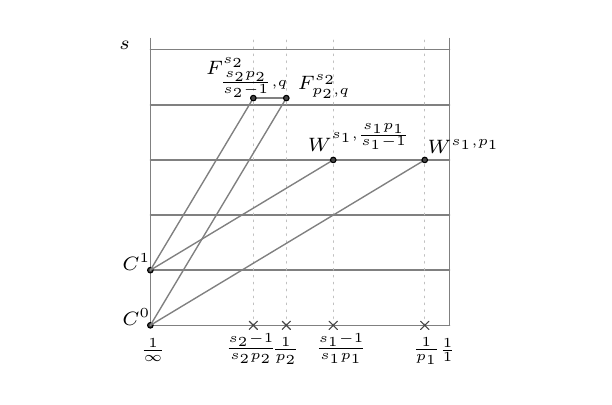
\begin{tikzpicture}[line cap=round,line join=round,>=triangle 45,x=3.8cm,y=0.7cm]
\clip(-0.41,-0.9277074696345513) rectangle (1.45,5.4);
%Quadricula
\draw [line width=.5pt,color=grisfosc] (0.,0.) -- (0.,5.203518980893238);
\draw [line width=.5pt,color=grisfosc] (1.,0.) -- (1.,5.203518980893238);
\draw [line width=.5pt,color=grisfosc] (0.,5.)-- (1.,5.);
\draw [line width=.5pt,color=grisfosc] (0.,3.)-- (1.,3.);
\draw [line width=.5pt,color=grisfosc] (0.,4.)-- (1.,4.);
\draw [line width=.5pt,color=grisfosc] (0.,2.)-- (1.,2.);
\draw [line width=.5pt,color=grisfosc] (0.,1.)-- (1.,1.);
\draw [line width=.5pt,color=grisfosc] (0.,0.)-- (1.,0.);
\begin{scriptsize}
\draw (-0.13,5.3) node[anchor=north west] {$s$};
\draw (0.94,-0.1) node[anchor=north west] {$\frac11$};
\draw (-0.06,-0.1) node[anchor=north west] {$\frac1\infty$};
\draw (-0.12,0.45) node[anchor=north west] {$C^0$};
\draw (-0.12,1.45) node[anchor=north west] {$C^1$};
\draw [fill=uuuuuu] (0.,1.) circle (1.0pt);
\draw [fill=uuuuuu] (0.,0.) circle (1.0pt);
\end{scriptsize}
%Vertical lines
\draw [line width=0.5pt,dotted,color=cqcqcq] (0.3441557837739109,0.) -- (0.3441557837739109,5.203518980893241);
\draw [line width=0.5pt,dotted,color=cqcqcq] (0.45437183207571896,0.) -- (0.45437183207571896,5.203518980893241);
\draw [line width=0.5pt,dotted,color=cqcqcq] (0.6113256095254408,0.) -- (0.6113256095254408,5.203518980893241);
\draw [line width=0.5pt,dotted,color=cqcqcq] (0.9169884142881612,0.) -- (0.9169884142881612,5.203518980893241);
\begin{scriptsize}
\draw (0.22438999981632807,0) node[anchor=north west] {$\frac{s_2-1}{s_2p_2}$};
\draw (0.38,-.08) node[anchor=north west] {$\frac1{p_2}$};
\draw (0.525339918478971,0) node[anchor=north west] {$\frac{s_1-1}{s_1p_1}$};
\draw (0.85,-.08) node[anchor=north west] {$\frac1{p_1}$};
\draw [color=uuuuuu] (0.3441557837739109,0.)-- ++(-1.5pt,-1.5pt) -- ++(3.0pt,3.0pt) ++(-3.0pt,0) -- ++(3.0pt,-3.0pt);
\draw [color=uuuuuu] (0.6113256095254408,0.)-- ++(-1.5pt,-1.5pt) -- ++(3.0pt,3.0pt) ++(-3.0pt,0) -- ++(3.0pt,-3.0pt);
\draw [color=uuuuuu] (0.45437183207571896,0.)-- ++(-1.5pt,-1.5pt) -- ++(3.0pt,3.0pt) ++(-3.0pt,0) -- ++(3.0pt,-3.0pt);
\draw [color=uuuuuu] (0.9169884142881612,0.)-- ++(-1.5pt,-1.5pt) -- ++(3.0pt,3.0pt) ++(-3.0pt,0) -- ++(3.0pt,-3.0pt);
\end{scriptsize}

%Triebel-Lizorkin scale
\draw [line width=.5pt,color=grisfosc]  (0.3441557837739109,4.122556007737622)-- (0.,1.);
\draw [line width=.5pt,color=grisfosc]  (0.45437183207571896,4.122556007737622)-- (0.,0.);
\draw [line width=.5pt,color=grisfosc]  (0.3441557837739109,4.122556007737622)-- (0.45437183207571896,4.122556007737622);
\begin{scriptsize}
\draw [fill=uuuuuu] (0.3441557837739109,4.122556007737622) circle (1.0pt);
\draw [fill=uuuuuu] (0.45437183207571896,4.122556007737622) circle (1.0pt);
\draw (0.4669924852688668,4.687604834614424) node[anchor=north west] {$F^{s_2}_{p_2,q}$};
\draw (0.16, 5) node[anchor=north west] {$F^{s_2}_{\frac{s_2p_2}{s_2-1},q}$};
\end{scriptsize}

%Sobolev scale
\draw [line width=.5pt,color=grisfosc]  (0.,1.)-- (0.6113256095254408,3.);
\draw [line width=.5pt,color=grisfosc]  (0.,0.)-- (0.9169884142881612,3.);
\draw [line width=.5pt,color=grisfosc]  (0.6113256095254408,3.)-- (0.9169884142881612,3.);
\begin{scriptsize}
\draw [fill=uuuuuu] (0.6113256095254408,3.) circle (1.0pt);
\draw [fill=uuuuuu] (0.9169884142881612,3.) circle (1.0pt);
\draw (0.9,3.5206561704123396) node[anchor=north west] {$W^{s_1,p_1}$};
\draw (0.5,3.8) node[anchor=north west] {$W^{s_1,\frac{s_1p_1}{s_1-1}}$};
\end{scriptsize}
\end{tikzpicture}
\end{figure}


\begin{lemma}\label{theoTriebelAdmissibleBanachBisBisBis}
Let $0<s<\infty$, $s\notin \N$, let $ 1\leq p < \infty$,  $ 1\leq q \leq \infty$ and $d\in\N$. Given bounded Lipschitz domains $\Omega_j\subset \R^d$ and a bi-Lipschitz function $f$ with $f(\Omega_1)= \Omega_2$, then 
\begin{align}\label{eqInvarianceUnderbiLipschitzTRIEBELBisBis}
 f \in \mathbf{F}^{s}_{\frac{ps}{s-1},q}(\Omega_1)\mbox{ and } g \in F^{s}_{p,q}\cap L^\infty(\Omega_2) &\implies   g \circ f \in F^{s}_{p,q}(\Omega_1)
\end{align}
(see Figure \ref{figComposition})
\end{lemma}

\begin{proof}
The proof is just a modification of the proof of \rf{eqInvarianceUnderbiLipschitzTRIEBELBis}. One has to set ${p_0}=\frac{ps}{i+\sigma}$ and ${p_j}=\frac{ps}{\alpha_j-1}$ in \squared{$2i\alpha$}, ${p_0}=\frac{ps}{i}$, ${p_r}=\frac{ps}{\alpha_r+\sigma/u_r-1}$, ${p_e}=\frac{ps}{\alpha_e-1}$ and $u_r=\frac{M}{\alpha_r-1}$ in 
\squared{$3i\alpha\ell\nu$} and ${p_0}=\frac{ps}{i+\sigma/u_0}$, ${p_r}=\frac{ps}{\alpha_r+\sigma/u_r-1}$, ${p_e}=\frac{ps}{\alpha_e-1}$,  $u_0=\frac{M+i}{i}$ and $u_r=\frac{M+i}{\alpha_r-1}$ in \squared{$4i\alpha\ell\nu$}. We leave the details to the reader.
\end{proof}

\begin{remark}The precise dependence obtained in the preceeding proofs is 
$$\norm{g \circ f }_{F^{s}_{p,q}(\Omega_1)} \leq C_{f} \left( \norm{g}_{F^{s}_{p,q}(\Omega_2)}\norm{\nabla f}_\infty^{s} + \norm{\nabla g}_\infty\norm{f}_{F^{s}_{p,q}(\Omega_1)}\right),$$
where
$$C_{f}=\left(1+\norm{\nabla f^{-1}}_\infty^{\frac dp} \right)\left(1+\norm{\nabla f^{-1}}_\infty^d \norm{\nabla f}_\infty^{d}\right),$$
and
$$\norm{g \circ f }_{F^{s}_{p,q}(\Omega_1)} \leq C_{f} \left( \norm{g}_{F^{s}_{p,q}(\Omega_2)}\left(\norm{\nabla f}_\infty^\frac s{s-1}\right)^{s} + \norm{g}_\infty \norm{f}_{F^{s}_{\frac{ps}{s-1},q}(\Omega_1)}^\frac{s}{s-1}\right),$$
where
$$C_{f}=\norm{\nabla f}_\infty^\frac{-s}{s-1}\left(\norm{\nabla f^{-1}}_\infty^{\frac d{ps}}+\norm{\nabla f^{-1}}_\infty^{\frac dp} \right)\left(1+\norm{\nabla f^{-1}}_\infty^d \norm{\nabla f}_\infty^{d}\right)$$

\end{remark}




\begin{proof}[Proof of \rf{eqInvarianceUnderInversionTRIEBELBis}]
Inequality \rf{eqInvarianceUnderInversionTRIEBELBis} is proven by analogous techniques using \rf{eqInverseDerivatives} and \rf{eqDerivativesInverse} which apply by Lemma \ref{lemSobolevAdmissibleSpace}. We claim that it is enough to check that $g_{ij}\in F^{s-1}_{p,q}(\Omega_1)$. Indeed, in case $1<s<2$, then we have that $f^{-1}$ is a bi-Lipschitz change of variables and, therefore, $g_{ij}\circ (f^{-1})\in F^{s-1}_{p,q}(\Omega_2)$ if and only if $g_{ij}\in F^{s-1}_{p,q}(\Omega_1)$.
Otherwise, by Lemma \ref{lemReadyForHolderInequality} we have that  $f\in F^{s-1}_{\frac{p(s-1)}{s-2},q}(\Omega_1)$. Inductively we can assume that $f^{-1}\in F^{s-1}_{\frac{p(s-1)}{s-2},q}(\Omega_1)$, and by \rf{eqInvarianceUnderbiLipschitzTRIEBELBisBis}, if $g_{ij}\in F^{s-1}_{p,q}(\Omega_1)$ then we get $g_{ij}\circ (f^{-1})\in F^{s-1}_{p,q}(\Omega_2)$ and  the claim follows.

Now, we want to prove
\begin{equation}\label{eqQuantifyInversion}
\circled{1}:=\left(\int_{\Omega_2} \left(\int_0^1 \frac{\left( \int_{U_{x,t}} |\nabla^{k-1} g_{ij}(x)-\nabla^{k-1} g_{ij}(y)| dy\right)^q}{t^{(\sigma+d)q}}\frac{dt}{t} \right)^\frac pq dx \right)^\frac1p \leq C_{f}\norm{f}_{\mathbf{F}^{s}_{p,q}(\Omega_1)}.
\end{equation}
where $U_{x,t}:=B(x,t)\cap\Omega_2$. Again we use first-order differences, and write $h:=y-x$.  For $|\alpha|=k+1$, we have
\begin{align*}
|\Delta_hD^\alpha g_{ij}(x)|
	& \lesssim \sum_{\beta, \gamma,\mu} \left| \frac{\prod_{\ell=1}^{k-1} D^{\gamma_\ell} f_{\mu_\ell}(x)}{\det(Df)^k(x)} \Delta_h(Df)^{\beta}(x) \right| \\
	& \quad\quad\quad +\left| (Df)^{\beta}(x+h) \prod_{\ell=1}^{k-1} D^{\gamma_\ell} f_{\mu_\ell}(x) \Delta_h \left(\frac{1}{\det(Df)^k}\right)(x)\right|\\
	& \quad\quad\quad+ \left|\frac{(Df)^{\beta}(x+h)}{\det(Df)^k(x+h)} \Delta_h\left(\prod_{\ell=1}^{k-1}  D^{\gamma_\ell} f_{\mu_\ell} (x)\right)\right|
\end{align*}
Now we use some trivial properties of first order differences, together with \rf{eqDifferencesProduct} to get
\begin{align*}
|\Delta_hD^\alpha g_{ij}|
	&\lesssim \sum_{\gamma,\mu}\norm{\nabla f}_\infty^{(d-1)k-1}\norm{\nabla f^{-1}}_\infty^{dk} |\Delta_h(D f)| \prod_{\ell=1}^{k-1} |D^{\gamma_\ell} f_{\mu_\ell}|   \\
	& \quad + \norm{\nabla f}_\infty^{(d-1)k}\norm{\nabla f^{-1}}_\infty^{d(k+1)}| \Delta_h \det(D f) | \prod_{\ell=1}^{k-1} |D^{\gamma_\ell} f_{\mu_\ell}|\\
	& \quad+ \norm{\nabla f}_\infty^{(d-1)k}\norm{\nabla f^{-1}}_\infty^{dk} \sum_{\nu\in\{0,1\}^{k-1}:|\nu|\geq 1} \prod_{r\leq k-1:\nu_r=1} |\Delta_hD^{\gamma_r} f_{\mu_r} |\prod_{e\leq k-1:\nu_e=0} |D^{\gamma_e} f_{\mu_e} |.
\end{align*}
To end, note that $|\Delta_h \det(D f)|\leq c \norm{\nabla f}_\infty^{d-1}|\Delta_h(Df)|$, so
\begin{align*}
|\Delta_hD^\alpha g_{ij}|
	&\lesssim \sum_{\gamma,\mu} \left(\norm{\nabla f}_\infty^{(d-1)k-1}\norm{\nabla f^{-1}}_\infty^{dk} + \norm{\nabla f}_\infty^{(d-1)k+d-1}\norm{\nabla f^{-1}}_\infty^{d(k+1)}\right)|\Delta_h(D f)| \prod_{\ell=1}^{k-1} |\nabla^{|\gamma_\ell|} f|   \\
	& \quad+ \norm{\nabla f}_\infty^{(d-1)k}\norm{\nabla f^{-1}}_\infty^{dk} \sum_{\nu\in\{0,1\}^{k-1}:|\nu|\geq 1} \prod_{r\leq k-1:\nu_r=1} |\Delta_h \nabla^{|\gamma_r|} f |\prod_{e\leq k-1:\nu_e=0} |\nabla^{|\gamma_e|} f |.
\end{align*}

Therefore, we write
\begin{align*}
\circled{1}
	& \lesssim C_f \sum_{\substack{ \gamma\in(\N_0^d)^{k-1}\\ |\gamma_\ell|\geq 1\, \&\,\sum|\gamma_\ell|=2k-2}} \left( \left(1+\norm{\nabla f}_\infty^{d}\norm{\nabla f^{-1}}_\infty^{d} \right) \squared{$2\gamma$}+\norm{\nabla f}_\infty\sum_{\nu\in\{0,1\}^{k-1}:|\nu|\geq 1}\squared{$3\gamma\nu$}\right),
\end{align*}
with $C_f=\norm{\nabla f}_\infty^{(d-1)k-1}\norm{\nabla f^{-1}}_\infty^{dk} $, with  \squared{$2\gamma$} and \squared{$3\gamma\nu$} as defined below.

Regarding the first term,  by H\"older's inequality we have
\begin{align*}
\squared{$2\gamma$} 
	& := \left( \int_{\Omega_2} \left(\int_0^1 \frac{ \left( \int_{U_x^t} |\Delta_h(D f)(x)|  dh\right)^q }{t^{(\sigma+d)q}}\frac{dt}{t} \right)^\frac pq \prod_{\ell=1}^{k-1} |\nabla^{|\gamma_\ell|} f(x)|^p dx \right)^\frac1p\\
	& \lesssim \norm{D f}_{F^\sigma_{p_0,q}(\Omega_1)} \prod_{\ell=1}^{k-1}\norm{\nabla^{|\gamma_\ell|} f}_{L^{p_\ell}(\Omega_1)},
\end{align*}
where $\sum_0^{k-1}\frac1{p_\ell}=\frac1p$ and $U_x^t:=B(x,t)\cap \Omega-x$. In particular choose $p_0=\frac{p(s-1)}{\sigma}$ and $p_\ell=\frac{p(s-1)}{|\gamma_\ell|-1}$. By Lemma \ref{lemReadyForHolderInequality} we get
\begin{align*}
\squared{$2\gamma$} 
	& \lesssim \norm{f}_{F^s_{p,q}(\Omega_1)}^{\frac{\sigma}{s-1}+\sum_\ell\frac{|\gamma_\ell|-1}{s-1}}\norm{\nabla f}_\infty^{\frac{s-1-\sigma}{s-1}+\sum_\ell\frac{s-|\gamma_\ell|}{s-1}} \\
	& =\norm{f}_{F^s_{p,q}(\Omega_1)}^{\frac{\sigma+k-1}{s-1}}\norm{\nabla f}_\infty^{\frac{s-1-\sigma +s(k-1)-(2k-2)}{s-1}} =\norm{f}_{F^s_{p,q}(\Omega_1)}\norm{\nabla f}_\infty^{k-1} 
\end{align*}

On the other hand, by H\"older's inequality again
\begin{align*}
\squared{$3\gamma\nu$} 
	& := \left( \int_{\Omega_2} \left(\int_0^1 \frac{ \left( \int_{U_{x,t}} \prod_{r\leq k-1:\nu_r=1} |\Delta_h \nabla^{|\gamma_r|} f  (x)|dh\right)^q }{t^{(\sigma+d)q}}\frac{dt}{t} \right)^\frac pq \prod_{e\leq k-1:\nu_e=0} |\nabla^{|\gamma_e|} f (x)|^p dx \right)^\frac1p\\
	& \lesssim \prod_r \norm{\nabla^{|\gamma_r|} f}_{F^{\sigma/u_r}_{p_r,q_r}(\Omega_1)} \prod_{e}\norm{\nabla^{|\gamma_\ell|} f}_{L^{p_e}(\Omega_1)},
\end{align*}
where we assume that $\sum_r \frac1{u_r}=\sum_1^{k-1} \frac{p}{p_{j}}=1$, $q_r:=u_r q$, as long as $1\leq u_r\leq \min\{p_r,q_r\} \frac{d+\sigma}{d}$. 

The fact that $u_r\leq q_r$ is clear from the definition of $q_r$. 
Let us write $M=\sum_r(|\gamma_r|-1)$ and define $u_r:= \frac{M}{|\gamma_r| - 1}$, $p_r=\frac{p(s-1)}{|\gamma_r|+\sigma/u_r -1}$ and $p_e=\frac{p(s-1)}{|\gamma_e|-1}$. Note that $\sum \frac1{u_r}=1$ and  $1\leq u_r$ trivially, while the condition $u_r \leq p_r$ is equivalent to $u_r(|\gamma_r|-1)\leq p(s-1) -\sigma$, that is, equivalent to $M\leq p(s-1) -\sigma$. But $M\leq |\gamma|-(k-1)= k-1=s-1-\sigma\leq p(s-1) -\sigma$, and thus it follows that $u_r\leq p_r$.

By Lemma \ref{lemReadyForHolderInequality} we get
\begin{align*}
\squared{$3\gamma\nu$} 
	& \lesssim \norm{f}_{F^s_{p,q}(\Omega_1)}^{\sum_r\frac{|\gamma_r|+\sigma/u_r-1}{s-1}+\sum_e\frac{|\gamma_e|-1}{s-1}}\norm{\nabla f}_\infty^{\sum_r\frac{s-|\gamma_r|-\sigma/u_r}{s-1}+\sum_e\frac{s-|\gamma_e|}{s-1}} \\
	& =\norm{f}_{F^s_{p,q}(\Omega_1)}^{\frac{\sigma+k-1}{s-1}}\norm{\nabla f}_\infty^{\frac{s(k-1)-(2k-2)-\sigma}{s-1}} =\norm{f}_{F^s_{p,q}(\Omega_1)}\norm{\nabla f}_\infty^{k-2} .
\end{align*}
All in all, 
\begin{align*}
\circled{1}
	& \lesssim \norm{\nabla f}_\infty^{dk-2}\norm{\nabla f^{-1}}_\infty^{dk}   \left( \left(1+\norm{\nabla f}_\infty^{d}\norm{\nabla f^{-1}}_\infty^{d} \right) \right)\norm{f}_{F^s_{p,q}(\Omega_1)}.
\end{align*}

\end{proof}


%Note that the proof that $g_{ij} \in F^{s-1}_{p,q}$ can also be done by using the algebra structure of $F^{s-1}_{p,q}\cap C^0$ and the fact that $\det(Df)^{-1}\in F^{s-1}_{p,q}$. The complexity of the proof is similar anyway. 

\section{Corkscrew and uniform domains}\label{secUniform}

\begin{definition}\label{defWhitney}
Given a domain $\Omega$, we say that a collection of open dyadic cubes $\mathcal{W}$ is a {\rm Whitney covering} of $\Omega$ if they are disjoint, the union of the cubes and their boundaries is $\Omega$, there exists a constant $C_{\mathcal{W}}$ such that 
$$C_\mathcal{W} \ell(Q)\leq \Dist(Q, \partial\Omega)\leq 4C_\mathcal{W}\ell(Q),$$
and the family $\{50 Q\}_{Q\in\mathcal{W}}$ has finite superposition. Moreover, we will assume that 
\begin{equation}\label{eqWhitney5}
S\subset 5Q \implies \ell(S)\geq \frac12 \ell(Q).
\end{equation}
\end{definition}
The existence of such a covering is granted for any open set different from $\R^d$ and in particular for any domain as long as $C_\mathcal{W}$ is big enough (see \cite[Chapter 1]{SteinPetit} for instance).

\begin{definition}
We say that a domain $\Omega\subset \R^d$ is an \emph{interior (resp. exterior) $(\varepsilon,\delta)$-corkscrew domain} if there is a Whitney covering of $\Omega$ (resp. $\overline{\Omega}^c$) such that given any ball $B(x,r)$ centered at $\partial\Omega$ with $0<r\leq \delta$ there exists a Whitney cube $Q\subset B(x,r)$ such that $\ell(Q)\geq \varepsilon r$.
\end{definition}



\begin{definition}\label{defEpsilonAdmissible}
Let $\Omega$ be a domain, $\mathcal{W}$ a Whitney decomposition of $\Omega$ and $Q,S\in\mathcal{W}$.  Given $M$ cubes $Q_1,\dots,Q_M\in\mathcal{W}$ with $Q_1=Q$ and $Q_M=S$, the $M$-tuple $(Q_1,\dots,Q_M)\in\mathcal{W}^M$  is a {\em chain} connecting $Q$ and $S$ if the cubes $Q_j$ and $Q_{j+1}$ are neighbors for $j<M$. We write $[Q,S]=(Q_1,\dots,Q_M)$ for short.

Let $\varepsilon\in\R$. We say that the chain $[Q,S]$ is {\em $\varepsilon$-admissible} if 
\begin{itemize}
\item the \emph{length}  of the chain is bounded by
\begin{equation}\label{eqLengthDistance}
\ell([Q,S]):=\sum_{j=1}^M\ell(Q_j)\leq \frac1\varepsilon\Dist(Q,S)
\end{equation}
\item and there exists $j_0<M$ such that the cubes in the chain satisfy
\begin{equation}\label{eqAdmissible1}
\ell(Q_j)\geq\varepsilon \Dist(Q_1,Q_j) \mbox{ for all } j\leq j_0 \mbox{\quad\quad  and \quad\quad }
\ell(Q_j)\geq\varepsilon \Dist(Q_j,Q_M) \mbox{ for all } j\geq j_0 .
\end{equation}
\end{itemize}
The $j_0$-th cube, which we call \emph{central}, satisfies that $\ell(Q_{j_0})\gtrsim_d \varepsilon \Dist(Q,S)$ by \rf{eqAdmissible1} and the triangle inequality. We will write  $Q_S=Q_{j_0}$. Note that this is an abuse of notation because the central cube of $[Q,S]$ may vary for different $\varepsilon$-admissible chains joining $Q$ and $S$.

We write (abusing notation again) $[Q,S]$ also for the set $\{Q_j\}_{j=1}^M$. Thus, we will write $P\in[Q,S]$ if $P$ appears in a coordinate of the $M$-tuple $[Q,S]$.
\end{definition}

Consider a domain $\Omega$ with covering $\mathcal{W}$ and two cubes $Q,S\in\mathcal{W}$ with an $\varepsilon$-admissible chain $[Q,S]$. From Definition \ref{defEpsilonAdmissible} it follows that
\begin{equation}\label{eqAdmissible2}
\Dist(Q,S)\approx_{\varepsilon,d} \ell([Q,S])\approx_{\varepsilon,d} \ell(Q_S).
\end{equation}
%
%If $P\in[Q,Q_S]$, by  \rf{eqAdmissible1} we have that 
%\begin{equation}\label{eqDistanceBoundedByLP} 
%\Dist(Q,P)\approx_{d,\varepsilon} \ell(P).
%\end{equation}
%On the other hand we have that
%\begin{equation}\label{eqNotVeryFar}
%\Dist(P,S)\approx_{\varepsilon,d} \Dist(Q,S).
%\end{equation}
 
\begin{definition}\label{defUniform}
We say that a domain $\Omega\subset\R^d$ is a {\em uniform domain} if there exists a Whitney covering $\mathcal{W}$ of $\Omega$ and $\varepsilon, \delta \in\R$ such that for any pair of cubes $Q,S \in\mathcal{W}$ with $\Dist(Q,S)\leq \delta$, there exists an $\varepsilon$-admissible chain $[Q,S]$. Sometimes we will write {\em $(\varepsilon,\delta)$-uniform domain} to fix the constants.
\end{definition}
 
Note that a uniform domain is also an interior corkscrew domain, perhaps with smaller  parameters.
 
For $1\leq j_1\leq j_2\leq M$, the subchain $[Q_{j_1},Q_{j_2}]_{[Q,S]} \subset[Q,S]$ is defined as $(Q_{j_1},Q_{j_1+1},\dots,Q_{j_2})$. We will write $[Q_{j_1},Q_{j_2}]$ if there is no risk of confusion.
Now we can define the shadows:
\begin{definition}\label{defShadow}
Let $\Omega$ be an $(\varepsilon,\delta)$-uniform domain with Whitney covering $\mathcal{W}$. 
Given a cube $P\in\mathcal{W}$ centered at $x_P$ and a real number $\rho$,  the {\em $\rho$-shadow} of $P$ is the collection of cubes
$$\SH_\rho(P)=\{Q\in\mathcal{W}:Q\subset B(x_P,\rho\,\ell(P))\}, $$
and its  {\em ``realization''} is the set
$$\Sh_{\rho}(P)=\bigcup_{Q\in\SH_\rho(P)} Q.$$

By the previous remark and the properties of the Whitney covering, we can define $\rho_\varepsilon>1$ such that the following properties hold:
\begin{itemize}
\item For every $\varepsilon$-admissible chain $[Q,S]$, and every $P\in[Q,Q_S]$ we have that $Q\in\SH_{\rho_\varepsilon}(P)$.
\item Moreover, every cube $P$ belonging to an $\varepsilon$-admissible chain $[Q,S]$ belongs to the shadow $\SH_{\rho_\varepsilon}(Q_S)$.
\end{itemize}
\end{definition}


\begin{remark}[see {\cite[Remark 2.6]{PratsSaksman}}]
\label{remInTheShadow}
Given an $(\varepsilon,\delta)$-uniform domain $\Omega$ we will write $\Sh$ for $\Sh_{\rho_\varepsilon}$. We will write also $\SH$ for $\SH_{\rho_{\varepsilon}}$.

For $Q\in\mathcal{W}$ and $s>0$,  we have that  
\begin{equation}\label{eqAscendingToGlory}
 \sum_{L: Q\in \SH(L)}\ell(L)^{-s} \lesssim \ell(Q)^{-s} \quad\quad\mbox{ and }\quad\quad  \sum_{\substack{L: Q\in \SH(L)\\\ell(L)\leq \rho}}\ell(L)^{s} \lesssim \rho^{s}
 \end{equation}
and, moreover, if $Q\in\SH(P)$ and $\Dist(Q,P)\leq \delta$, then
\begin{equation}\label{eqAscendingPath}
 \sum_{L\in[Q,P]}\ell(L)^{s} \lesssim \ell(P)^s \mbox{\quad\quad and \quad\quad}  \sum_{L\in[Q,P]}\ell(L)^{-s}\lesssim \ell(Q)^{-s} .
 \end{equation}
\end{remark}
Note that the property \rf{eqAscendingToGlory} is not a consequence of uniformity, but of the definition of shadow. 


We recall the definition of the non-centered Hardy-Littlewood maximal operator. Given $f\in L^1_{loc}(\R^d)$ and $x\in\R^d$, we define $Mf(x)$ as the supremum of the mean of $f$ in cubes containing $x$, that is,
$$Mf(x)=\sup_{Q:  x\in Q} \frac{1}{|Q|} \int_Q f(y) \, dy.$$
It is a well known fact that this operator is bounded in $L^p$ for $1<p<\infty$.
The following lemma is proven in \cite{PratsTolsa} and will be used repeatedly along the proofs contained in the present text.

\begin{lemma}\label{lemMaximal}
Let $\Omega$ be a  domain with Whitney covering $\mathcal{W}$. Assume that $g\in L^1(\Omega)$ and $r>0$. For every $\eta>0$, $Q\in\mathcal{W}$ and $x\in \R^d$, we have
\begin{enumerate}[1)]
\item The non-local {inequalities} for the maximal operator
	\begin{equation}\label{eqMaximalFar}
	 \int_{|y-x|>r} \frac{g(y) \, dy}{|y-x|^{d+\eta}}\lesssim_d \frac{Mg(x)}{r ^\eta}
\mbox{\quad\quad and \quad\quad}
	 \sum_{S:\Dist(Q,S)>r}  \frac{\int_S g(y) \, dy}{\Dist(Q,S)^{d+\eta}}\lesssim_d \frac{\inf_{y\in Q} Mg(y)}{r ^\eta}.
	 \end{equation}
\item The local {inequalities} for the maximal operator
	\begin{equation}\label{eqMaximalClose}
	 \int_{|y-x|<r} \frac{g(y) \, dy}{|y-x|^{d-\eta}}\lesssim_d r ^\eta Mg(x)
\mbox{\quad\quad and \quad\quad}
	\sum_{S:\Dist(Q,S)<r}  \frac{\int_S g(y) \, dy}{\Dist(Q,S)^{d-\eta}}\lesssim_d \inf_{y\in Q} Mg(y) \,r^\eta.
	 \end{equation}
\item In particular, if $\Omega$ is a uniform domain, we have
	\begin{equation}\label{eqMaximalAllOver}
		\sum_{S\in\mathcal{W}} \frac{\ell(S)^d}{\Dist(Q,S)^{d+\eta}} \lesssim_d \frac{1}{\ell(Q)^\eta}
\mbox{\quad\quad and \quad\quad}
		\sum_{S\in \SH_{{\rho}}(Q)} \ell(S)^{d} \lesssim_{d,\rho} \ell(Q)^d
	\end{equation}
and, by Definition \ref{defShadow},
	\begin{equation}\label{eqMaximalGuay}
	\sum_{S\in\SH_{{\rho}} (Q)} \int_S g(x) \, dx\lesssim_{d,\rho} \inf_{y\in Q} Mg(y) \, \ell(Q)^d.
	 \end{equation}
\end{enumerate}
\end{lemma}



\section{Extension operators}\label{secExtension}
\begin{definition}\label{defAspqU}
Consider $1\leq p<\infty$, $1\leq q \leq \infty$, $1\leq u \leq \infty$ and $0<\sigma<1$ so that $\sigma> \frac{d}{\min\{p,q\}}-\frac{d}{u}$. Let $U$ be an open set in $\R^d$. We say that a locally integrable function $f\in F^{\sigma,\rho}_{p,q,u}(U)$ if
\begin{itemize}
\item The function $f\in L^p(U)$, and
\item the seminorm
\begin{equation}\label{eqSeminormAspq}
\norm{f}_{\dot{F}^{\sigma,\rho}_{p,q,u}(U)}:=\left(\int_U\left(\int_0^\rho \frac{\left(\int_{U_{x,t}} |f(x)-f(y)|^u\right)^\frac qu}{t^{\sigma q+\frac{dq}{u}}} \,\frac{dt}{t} \right)^{\frac{p}{q}}dx\right)^{\frac{1}{p}}
\end{equation}
is finite, where we denote $U_{x,t}:=B(x,t)\cap U$. 
\end{itemize}
We define the norm 
\begin{equation*}
\norm{f}_{{F}^{\sigma,\rho}_{p,q,u}(U)}:=\norm{f}_{L^p(U)}+\norm{f}_{\dot{F}^{\sigma,\rho}_{p,q,u}(U)}.
\end{equation*}
For $s=k+\sigma$ with $k\in\N$, we write
\begin{equation*}
\norm{f}_{{F}^{s,\rho}_{p,q,u}(U)}:=\norm{f}_{W^{k,p}(U)}+\norm{\nabla^k f}_{\dot{F}^{\sigma,\rho}_{p,q,u}(U)}.
\end{equation*}
\end{definition}

In order to prove that $F^s_{p,q}(\Omega)=F^{s,1}_{p,q,u}(\Omega)$ for a given domain $\Omega$, it suffices to find an extension operator $\mathcal{E}:F^{s,\rho}_{p,q,1}(\Omega)\to F^{s,1}_{p,q,1}(\R^d)$ with $\rho<1$. Once this is established, using the equivalence of norms in the ambient space (see \cite[Theorem 1.116]{TriebelTheoryIII}) we obtain the equivalence of norms in the domain by classical arguments:

First note that 
\begin{equation}\label{eqCompareNormsRadius}
\norm{g}_{F^{s}_{p,q}(\R^d)}\approx\norm{g}_{F^{s,1}_{p,q,u}(\R^d)}\approx\norm{g}_{F^{s,\rho}_{p,q,u}(\R^d)}.
\end{equation}
First comparison comes from \cite[Theorem 1.116]{TriebelTheoryIII}. The second can be obtained easily by using the change of variables $\widetilde{x}=\rho^{-1}x$, $\widetilde{t}=\rho^{-1}t$, $\widetilde{y}=\rho^{-1}y$ in the last norm and then compare the norms of $g$ and its rescaling $g(\rho\cdot)$  in $F^s_{p,q}$. 

Thus, 
$$\inf_{g|_\Omega \equiv f} \norm{g}_{F^s_{p,q}(\R^d)}\leq \norm{\mathcal{E}f}_{F^s_{p,q}(\R^d)} \approx \norm{\mathcal{E}f}_{F^{s,1}_{p,q,1}(\R^d)}\lesssim  \norm{f}_{F^{s,\rho}_{p,q,1}(\Omega)}\lesssim  \norm{f}_{F^{s,\rho}_{p,q,u}(\Omega)}\leq \inf_{g|_\Omega \equiv f}\norm{g}_{F^{s,\rho}_{p,q,u}(\R^d)}.$$
Since the first and the last are comparable (with constants independent of $\rho$) it follows that all the quantities are comparable and, in particular, 
$$F^s_{p,q}(\Omega)=F^{s,\rho}_{p,q,u}(\Omega).$$

To end, since $\rho<1$ then 
$$\norm{f}_{F^{s,\rho}_{p,q,u}(\Omega)}\leq \norm{f}_{F^{s,1}_{p,q,u}(\Omega)}\leq  \norm{\mathcal{E} f}_{F^{s,1}_{p,q,u}(\R^d)}\lesssim \norm{f}_{F^{s,\rho}_{p,q,u}(\Omega)}.$$

\subsection{Corkscrew domains and smoothness below one}\label{secCorkscrew}
Let $\Omega$ be an interior corkscrew domain. To define the extension operator we need a Whitney covering $\mathcal{W}_0$ of $\Omega$ and we define $\mathcal{W}_1$ to be the collection of cubes in $\mathcal{W}_0$ with side-length smaller than $c_0\ell_0<<\delta\wedge 1$, a Whitney covering $\mathcal{W}_2$ of $\Omega^c$ and we define $\mathcal{W}_3$ to be the collection of cubes in $\mathcal{W}_2$ with side-lengths smaller than $10 \ell_0$, so that for any $Q\in \mathcal{W}_3$ there is a $S\in \mathcal{W}_1$ with $\Dist(Q,S)\leq C \ell(Q)$ and $\ell(Q)=\ell(S)$ (see \cite[Lemma 2.4]{Jones}). In case $\Omega$ is unbounded and $\delta=\infty$, choose $\ell_0=1$. We define the symmetrized cube $Q^*$ as one of the cubes satisfying these properties. Note that the number of possible choices for $Q^*$ is uniformly bounded.


\begin{lemma}\label{lemSymmetrized}[see \cite{Jones}]
Let $\Omega$ be an interior corkscrew domain. For cubes $Q_1,Q_2\in\mathcal{W}_3$ and $S\in\mathcal{W}_1$ we have that
\begin{itemize}
\item The symmetrized cubes have finite overlapping: there exists a constant $C$ depending on the parameter $\varepsilon$ and the dimension $d$ such that $\#\{Q\in\mathcal{W}_3: Q^*=S\}\leq C$.
\item The long distance is invariant in the following sense:
\begin{equation}\label{eqLongDistanceInvariant}
\Dist(Q_1^*,Q_2^*)\approx \Dist(Q_1,Q_2) \mbox{\quad\quad and \quad\quad}\Dist(Q_1^*,S)\approx \Dist(Q_1,S) 
\end{equation}
\end{itemize}
\end{lemma}

We define the family of bump functions $\{\psi_Q\}_{Q\in \mathcal{W}_2}$ to be a partition of the unity associated to $\left\{\frac{11}{10}Q\right\}_{Q\in\mathcal{W}_2}$, that is, their sum $\sum\psi_Q\equiv 1$, they satisfy the pointwise inequalities $0\leq \psi_Q\leq \chi_{\frac{11}{10}Q}$ and $\norm{\nabla\psi_Q}_\infty \lesssim \frac{1}{\ell(Q)}$.  We can define the operator
$$\Lambda_0 f(x)= f(x)\chi_\Omega(x) + \sum_{Q\in\mathcal{W}_3} \psi_Q(x) f_{Q^*} \mbox{ for any }f\in L^1_{loc}(\Omega)$$
 (here $f_{U}$ stands for the mean of a function $f$ in a set $U$). This function is defined almost everywhere because the boundary of the domain $\Omega$ has zero Lebesgue measure (see \cite[Lemma 2.3]{Jones}).





\begin{theorem}\label{theoExtensionOperator0}
Let $\Omega\subset\R^d$ be an interior $(\varepsilon,\delta)$-corkscrew domain, let $1\leq p<\infty$, $1\leq q\leq \infty$ and $0<s<1$. Then, $\Lambda_0: F^{s,C\ell_0}_{p,q,1}(\Omega)\to F^{s,1}_{p,q,1}(\R^d)$, with $C$ depending only on $d$ and $\varepsilon$ while $\ell_0$ depends also on $\delta$.
\end{theorem}

\begin{proof}
In light of \rf{eqCompareNormsRadius}, it is enough to check $\Lambda_0: F^{s,C\ell_0}_{p,q,1}(\Omega)\to F^{s,\ell_0}_{p,q,1}(\R^d)$ for $\ell_0$ small enough, that is
\begin{align*}
\norm{\Lambda_0 f}_{{F}^{s,\ell_0}_{p,q,1}(\R^d)}
	&=\norm{\Lambda_0 f}_{L^p}+ \norm{\norm{\frac{ \norm{\Lambda_0 f(x)-\Lambda_0 f(y)}_{L^1_y (B_{x,t})}}{t^{s+{d}+\frac1q}}}_{L^q_t(0,\ell_0)}}_{L^p_x(\R^d)} \lesssim \norm{f}_{F^{s,C\ell_0}_{p,q,1}(\Omega)},
\end{align*}
where $B_{x,t}:=B(x,t)$. 


First, note that $\norm{\Lambda_0f}_{L^p}\leq \norm{f}_{L^p(\Omega)}+\norm{\Lambda_0f}_{L^p(\Omega^c)}$. By Jensen's inequality, we have that 
$$\norm{\Lambda_0f}_{L^p(\Omega^c)}^p\lesssim_p \sum_{Q\in\mathcal{W}_3} |f_{Q^*}|^p\norm{\psi_Q}_{L^p}^p \leq \sum_{Q\in\mathcal{W}_3} \frac{1}{\ell(Q)^d}\norm{f}_{L^p(Q^*)}^p  \left(\frac{11}{10}\ell(Q)\right)^d . $$
By the finite overlapping of the symmetrized cubes, 
\begin{equation}\label{eqExtensionInLp}
\norm{\Lambda_0f}_{L^p(\Omega^c)}^p\lesssim \norm{f}_{L^p(\Omega)}^p. 
\end{equation}
%The same can be said about $L^u$ when $u>p$. In that case, moreover, one can cover $\Omega$ with balls $\{B_j\}_{j\in J}$ with radius one half such that $|B_j\cap\Omega|\approx 1$. Then, using the subadditivity of  $x\mapsto |x|^{\frac{p}{q}}$ we get
%\begin{align}\label{eqPimpliesQ}
%\norm{f}_{L^u(\Omega)}^p
%			& \leq \left(\sum_j \int_{B_j\cap \Omega}|f(y)|^u \, dy\right)^\frac{p}{u} \\
%\nonumber	& \lesssim_u \sum_j \left(\fint_{B_j\cap \Omega} \left(\int_{B_j\cap \Omega}|f(y)-f(x)|^u \, dy\right)^\frac{p}{u} dx + \fint_{B_j\cap \Omega}  \left(\int_{B_j\cap \Omega}|f(x)|^u \, dy\right)^\frac{p}{u}dx\right)
%\end{align}
%Now, using Minkowski's integral inequality and Jensen's inequality, we get  
%\begin{align*}
%\sum_j \int_{B_j\cap \Omega} \left(\int_{B_j\cap \Omega}|f(y)-f(x)|^u \, dy\right)^\frac{p}{u} dx 
%	&\lesssim \sum_j \int_{B_j\cap \Omega} \left(\int_{B_j\cap \Omega}|f(y)-f(x)|^u \left(\int_{|x-y|}^{\ell_0} dt \right)^u\, dy\right)^\frac{p}{u} dx \\
%	&\lesssim  \int_{ \Omega} \left(\int_{0}^{\ell_0} \left(\int_{\Omega_{x,t}}|f(y)-f(x)|^u  dy \right)^\frac qu dt\right)^\frac{p}{q} dx ,
%\end{align*}
%and 
%$$ \fint_{B_j\cap \Omega}  \left(\int_{B_j\cap \Omega}|f(x)|^u \, dy\right)^\frac{p}{u}dx \lesssim \norm{f}_{L^p(\Omega)}^p$$
%so
%\begin{align}\label{eqPimpliesQ}
%\norm{f}_{L^u(\Omega)}^p
%\nonumber	& \lesssim \norm{f}_{A^{s,\rho}_{p,q,u}(\Omega)}^p
%\end{align}
%for every $\rho\geq 1$.

 It remains to check that
\begin{equation*}
\norm{\Lambda_0 f}_{{\dot F}^{s,{\ell_0}}_{p,q,1}(\R^d)}= \norm{\norm{\frac{ \norm{\Lambda_0 f(x)-\Lambda_0 f(y)}_{L^1_y (B_{x,t})}}{t^{s+{d}+\frac1q}}}_{L^q_t(0,\ell_0)}}_{L^p_x(\R^d)}\lesssim \norm{f}_{F^{s,C{\ell_0}}_{p,q,1}(\Omega)}.
\end{equation*}
More precisely, we will prove that 
\begin{align*}
\circled{a}+\circled{b}+\circled{c} \lesssim \norm{f}_{F^{s,C\ell_0}_{p,q,1}(\Omega)},
\end{align*}
where
\begin{align*}
\circled{a} 
	& := \norm{\norm{\frac{ \norm{f(x)-\Lambda_0 f(y)}_{L^1_y (\Omega^c_{x,t})}}{t^{s+{d}+\frac1q}}}_{L^q_t(0,\ell_0)}}_{L^p_x(\Omega)}	,
\end{align*}
\begin{align*}
\circled{b} 
	& := \norm{\norm{\frac{ \norm{\Lambda_0f(x)- f(y)}_{L^1_y (\Omega_{x,t})}}{t^{s+{d}+\frac1q}}}_{L^q_t(0,\ell_0)}}_{L^p_x(\Omega^c)}
	\end{align*}
	and
\begin{align*}
\circled{c}
	& := \norm{\norm{\frac{ \norm{\Lambda_0f(x)- \Lambda_0f(y)}_{L^1_y (\Omega^c_{x,t})}}{t^{s+{d}+\frac1q}}}_{L^q_t(0,\ell_0)}}_{L^p_x(\Omega^c)}.
\end{align*}

Let us begin with 
\begin{align*}
\circled{a}
	& = \norm{\norm{\frac{ \norm{f(x)-\sum_{S\in\mathcal{W}_3} \psi_{S}(y) f_{S^*}}_{L^1_y (\Omega^c_{x,t})}}{t^{s+{d}+\frac1q}}}_{L^q_t(0,\ell_0)}}_{L^p_x(\Omega)}.
\end{align*}
Call $\mathcal{W}_4:=\{S\in\mathcal{W}_3: \mbox{ all the neighbors of $S$ are in } \mathcal{W}_3\}$. We write $ \mathcal{W}_j(Q,t):=\{S\in\mathcal{W}_j: S\cap \bigcup_{x\in Q} B_{x,t}\neq \emptyset \} $. 
Note that if $S\in\mathcal{W}_3(Q,t)$ with $Q\in \mathcal{W}_1$ and $t<\ell_0$, then $S\in \mathcal{W}_4$. Given $y\in \frac{11}{10}S$, where $S\in \mathcal{W}_4$, we have that $\sum_{P\in\mathcal{W}_3} \psi_P(y)\equiv 1$. Therefore
\begin{align*}
\circled{a}
	&  \leq \norm{\norm{\norm{\frac{ \sum_{S\in\mathcal{W}_4(Q,t)} |   f(x)- f_{S^*}| \int_{\frac{11}{10}S} \psi_{S}(y) \,dy}{t^{s+{d}+\frac1q}}}_{L^q_t(0,\ell_0)}}_{L^p_x(Q)}}_{\ell^p_Q(\mathcal{W}_{1})}
\\
%	& \quad + \left(\sum_{Q\in\mathcal{W}_1}\int_Q \left(\int_0^{\ell_0} \frac{\left(\sum_{S\in\mathcal{W}_2(Q,t)\setminus\mathcal{W}_4} \int_{\frac{11}{10}S}\left| \left(1- \sum_{P\in\mathcal{W}_3} \psi_P(y)\right)f(x)\right|\, dy \right)^q}{t^{sq+dq}} \,\frac{dt}{t}\right)^{\frac{p}{q}}dx\right)^{\frac{1}{p}}\\
%	&=:\circled{a1}+\circled{a2}.
\end{align*}
By the choice of the symmetrized cube we have that $\int_{\frac{11}{10}S}  \psi_{S}(y) \,dy \approx \ell(S^*)^d$. Thus,
\begin{align*}
\circled{a}
	& \lesssim_d \norm{\norm{\norm{\frac{\sum_{S\in\mathcal{W}_4(Q,t)} \int_{S^*}|f(x)-f(\xi)|\, d\xi}{t^{s+{d}+\frac1q}}}_{L^q_t(0,\ell_0)}}_{L^p_x(Q)}}_{\ell^p_Q(\mathcal{W}_{1})}
\end{align*}
By \rf{eqLongDistanceInvariant}, if $Q\in\mathcal{W}_1$ and $S\in \mathcal{W}_4(Q,t)$ then $S^*\in \mathcal{W}_1(Q, C_\Omega t)$ and using also the finite overlapping of the symmetrized cubes, we get that 
\begin{align*}
\circled{a}
	& \lesssim_{d,\varepsilon} \norm{\norm{\norm{\frac{\sum_{S\in\mathcal{W}_1(Q,C_\Omega t)} \int_{S}|f(x)-f(\xi)|\, d\xi}{t^{s+{d}+\frac1q}}}_{L^q_t(0,\ell_0)}}_{L^p_x(Q)}}_{\ell^p_Q(\mathcal{W}_{1})}\lesssim_{s,d}  \norm{f}_{\dot F^{s,C_\Omega}_{p,q,1}(\Omega)}.
\end{align*}
	
%To bound $\circled{a2}$ just note that for $Q\in\mathcal{W}_1$ and $S\in\mathcal{W}_2\setminus\mathcal{W}_4$, we have that $S$ is far from the boundary, say $\dist(S,Q)\geq C_\mathcal{W}\ell_0$, where $\ell_0$ depends only on $\diam(\Omega)$ and $\varepsilon$ if $\Omega$ is bounded. Thus, we have that
%$$\circled{a2}\lesssim \left(\sum_{Q\in\mathcal{W}_1}\int_Q \left(\int_{C_\mathcal{W}\ell_0}^{\ell_0} \frac{\left(\sum_{S\in\mathcal{W}_2(Q,t)} \int_{\frac{11}{10}S}\left| f(x)\right|\, dy \right)^q}{t^{sq+dq}} \,\frac{dt}{t}\right)^{\frac{p}{q}}dx\right)^{\frac{1}{p}}
% \lesssim \left(\int_{C_\mathcal{W}\ell_0}^{\ell_0} \frac{dt}{t^{sq+1}}\right)^\frac{1}{q}\norm{f}_{L^p}.$$


Next, note that, using the same reasoning as above and the finite superposition of the rescaled Whitney cubes, we have that
\begin{align*}
\circled{b}
	& = \norm{\norm{\frac{ \norm{\sum_{Q\in\mathcal{W}_3} \psi_{Q}(x) f_{Q^*}- f(y)}_{L^1_y (\Omega_{x,t})}}{t^{s+{d}+\frac1q}}}_{L^q_t(0,\ell_0)}}_{L^p_x(\Omega^c)}\\
	& \lesssim_{d,p} \norm{\norm{ \psi_Q(x) \norm{\frac{ \norm{ f_{Q^*}- f(y)}_{L^1_y (\Omega_{x,t})}}{t^{s+{d}+\frac1q}}}_{L^q_t(0,\ell_0)}}_{L^p_x(\frac{11}{10}Q)}}_{\ell^p_Q(\mathcal{W}_4)}.
%	&\quad + \left(\sum_{P\in\mathcal{W}_2\setminus\mathcal{W}_4}\int_{P}\left(1- \sum_{Q\in \mathcal{W}_3}\psi_{Q}(x) \right)^p  \left(\int_0^{\ell_0} \frac{\left(\int_{\Omega_{x,t}}\left| f(y)\right| dy\right)^q}{t^{sq+dq}} \,\frac{dt}{t}\right)^{\frac{p}{q}}dx\right)^{\frac{1}{p}}\\
%	& = :\circled{b1}+\circled{b2}.
\end{align*}
Taking absolute values inside and enlarging the integration domain in $y$ and computing the integral in $Q$, we have that
\begin{align*}
\circled{b}
	& \lesssim_{d,p} \norm{ \ell(Q)^\frac dp \norm{\frac{ \norm{\frac{1}{\ell(Q)^{d}} \norm{f(\xi)-f(y)}_{L^1_\xi(Q^*) }}_{L^1_y (\Omega_{Q,t})}}{t^{s+{d}+\frac1q}}}_{L^q_t(0,\ell_0)}}_{\ell^p_Q(\mathcal{W}_4)}\\
\end{align*}
where $\Omega_{Q,t}=\bigcup_{x\in Q}\Omega_{x,t}$. Thus, applying Fubini's theorem and  Minkowsky's integral inequality (see \cite[Appendix A1]{SteinPetit}), we get
\begin{align*}
\circled{b}
	& \lesssim_{d,p} \norm{ \frac{\ell(Q)^\frac dp}{\ell(Q)^{d}} \norm{\norm{\frac{ \norm{f(\xi)-f(y)}_{L^1_y (\Omega_{Q,t})}}{t^{s+{d}+\frac1q}}}_{L^q_t(0,\ell_0)}}_{L^1_\xi(Q^*) }}_{\ell^p_Q(\mathcal{W}_4)}.
\end{align*}
If $Q\in \mathcal{W}_4$ and $y\in \Omega_{Q,t}$, then $y\in\Omega_{\xi,C_\Omega t}$ for every $\xi\in Q^*$. By H\"older's inequality and the finite overlapping of symmetrized cubes, we get that
\begin{align*}
\circled{b}
	& \lesssim_{d,p,\varepsilon} \norm{ \norm{\norm{\frac{ \norm{f(\xi)-f(y)}_{L^1_y (\Omega_{\xi,C_\Omega t})}}{t^{s+{d}+\frac1q}}}_{L^q_t(0,\ell_0)}}_{L^p_\xi(Q) }}_{\ell^p_Q(\mathcal{W}_1)}	\lesssim  \norm{f}_{\dot F^{s,C_\mathcal{W}}_{p,q,1}(\Omega)}.
\end{align*}
	
%To bound $\circled{b2}$, we use that $\int_Pdx=\int_{P^*}dx$ and \rf{eqLongDistanceInvariant} again to get that
%\begin{align*}
%\circled{b2}
%	& \leq \left(\sum_{P\in\mathcal{W}_2\setminus\mathcal{W}_4} \int_{P^*} \left(\int_{C\ell_0}^{\ell_0} \frac{\left(\int_{\Omega_{P,t}}\left| f(y)-f(x)\right| dy\right)^q}{t^{sq+dq}} \,\frac{dt}{t}\right)^{\frac{p}{q}}  \,dx\right)^{\frac{1}{p}} \\
%	& \quad +  \left(\sum_{P\in\mathcal{W}_2\setminus\mathcal{W}_4} \int_{P^*} \left(\int_{C\ell_0}^{\ell_0} \frac{\left(\int_{\Omega_{P,t}} dy\right)^q}{t^{sq+dq}} \,\frac{dt}{t}\right)^{\frac{p}{q}}  \left| f(x)\right|^p\,dx\right)^{\frac{1}{p}} \\
%	& \leq \left(\int_{\Omega} \left(\int_{0}^{\ell_0} \frac{\left(\int_{\Omega_{x,C_\mathcal{W}t}}\left| f(y)-f(x)\right| dy\right)^q}{t^{sq+dq}} \,\frac{dt}{t}\right)^{\frac{p}{q}}  \,dx\right)^{\frac{1}{p}} +  \norm{f}_{L^p}  \left(\int_{C\ell_0}^{\ell_0}  \,\frac{dt}{t^{sq+1}}\right)^{\frac{1}{q}}  \\
%	& \lesssim \norm{f}_{F^{s,C_{\mathcal{W}}}_{p,q,u}}.
%\end{align*}


Let us focus on $\circled{c}$.  By the triangle inequality, we have that
\begin{align*}
\circled{c}
	& \leq \norm{ \norm{\norm{\frac{ \norm{\sum_{P\in\mathcal{W}_3} \psi_{P}(x) f_{P^*}-\sum_{S\in\mathcal{W}_3} \psi_{S}(y) f_{S^*}}_{L^1_y (\Omega^c_{x,t})}}{t^{s+{d}+\frac1q}}}_{L^q_t(\frac{\ell(Q)}{10},\ell_0)}}_{L^p_x(Q) }}_{\ell^p_Q(\mathcal{W}_4)}\\
	& \quad + \norm{ \norm{\norm{\frac{ \norm{\sum_{P\in\mathcal{W}_3} \psi_{P}(x) f_{P^*}-\sum_{S\in\mathcal{W}_3} \psi_{S}(y) f_{S^*}}_{L^1_y (\Omega^c_{x,t})}}{t^{s+{d}+\frac1q}}}_{L^q_t(0,\frac{\ell(Q)}{10})}}_{L^p_x(Q) }}_{\ell^p_Q(\mathcal{W}_4)}\\
	& \quad + \norm{ \norm{\norm{\frac{ \norm{\sum_{P\in\mathcal{W}_3} \psi_{P}(x) f_{P^*}-\sum_{S\in\mathcal{W}_3} \psi_{S}(y) f_{S^*}}_{L^1_y (\Omega^c_{x,t})}}{t^{s+{d}+\frac1q}}}_{L^q_t(0,\ell_0)}}_{L^p_x(Q) }}_{\ell^p_Q(\mathcal{W}_2\setminus\mathcal{W}_4)}\\
	& =: \circled{c1}+\circled{c2}+\circled{c3}
\end{align*}




%
%Finally, we will group the remaining cases, when $x\in\Omega^c$ and $y\notin  \Omega^c_{x,\ell_0}$ in an error term.
%Considering all these facts we get
%\begin{align*}	
%\circled{c}	
%	& 
%	& \quad+ 	& \quad+ 
%	& \quad+\left(\int_{\Omega^c} \left(\int_{1\wedge \ell_0}^{\ell_0} \frac{\left(\int_{\Omega^c_{x,t}} | \Lambda_0 f(x)-\Lambda_0 f(y)| dy\right)^q}{t^{sq+dq}} \,\frac{dt}{t}\right)^{\frac{p}{q}}dx\right)^{\frac{1}{p}} =: \circled{c4}\\
%\end{align*}
%where the last two terms vanish in case $\Omega$ is bounded. 

The first term is bounded using the same techniques as in $\circled{a}$ and $\circled{b}$. 
Indeed, given $x\in \frac{11}{10}Q$ where $Q\in \mathcal{W}_4$ and $y\in \Omega^c_{x, {\ell_0}/{10}}$, then neither $x$ nor $y$ are in the support of any bump function of a cube in $\mathcal{W}_2\setminus\mathcal{W}_3$, so $\sum_{S\in\mathcal{W}_3} \psi_S(y)\equiv 1$ and $\sum_{P\in\mathcal{W}_3} \psi_P(x)\equiv 1$. Therefore
$$\sum_{P\in\mathcal{W}_3} \psi_{P}(x) f_{P^*}-\sum_{S\in\mathcal{W}_3} \psi_{S}(y) f_{S^*}=  \sum_{P\cap 2Q\neq \emptyset}  \sum_{S\in\mathcal{W}_3} \psi_{P}(x)\psi_{S}(y)\left(f_{P^*}-f_{S^*}\right).$$
Using first the triangle inequality and the bounded number of neighboring cubes, and then computing the integral in $x$, taking absolute values inside the inner integral and changing the order of summation on $Q$ and $P$ we get
\begin{align*}
\circled{c1}
	&=\norm{ \norm{\norm{\frac{ \norm{\sum_{P\cap 2Q\neq \emptyset}  \sum_{S\in\mathcal{W}_3}\left|\psi_{P}(x) \psi_{S}(y)\right| \left|f_{P^*}- f_{S^*}\right|}_{L^1_y (\Omega^c_{x,t})}}{t^{s+{d}+\frac1q}}}_{L^q_t(\frac{\ell(Q)}{10},\ell_0)}}_{L^p_x(Q) }}_{\ell^p_Q(\mathcal{W}_4)}\\
	&  \lesssim_{d,p} \norm{\left(\sum_{P\cap 2Q\neq \emptyset} \norm{ \psi_{P}(x)\norm{\frac{ \sum_{S\in\mathcal{W}_3(P,C_dt)}\left|f_{P^*}- f_{S^*}\right| \ell(S)^d}{t^{s+{d}+\frac1q}}}_{L^q_t(\frac{\ell(Q)}{10},\ell_0)}}_{L^p_x(Q) }^p\right)^\frac1p}_{\ell^p_Q(\mathcal{W}_4)}\\
	&  \lesssim_d \norm{ \ell(P)^\frac dp \norm{\frac{  \sum_{S\in\mathcal{W}_3(P,C_dt)}  \frac{1}{\ell(P)^d}\norm{\norm{ f(\xi)- f(\zeta) }_{L^1_\zeta(S^*)}}_{L^1_\xi(P^*)}}{t^{s+{d}+\frac1q}}}_{L^q_t(\frac{\ell(P)}{20},\ell_0)}}_{\ell^p_P(\mathcal{W}_3)},
\end{align*}
and applying Minkowski's and Jensen's inequalities we obtain
\begin{align*}
\circled{c1}
	&\lesssim_{d,p}  \norm{ \norm{ \norm{\frac{  \sum_{S\in\mathcal{W}_3(P,C_dt)} \norm{ f(\xi)- f(\zeta) }_{L^1_\zeta(S^*)}}{t^{s+{d}+\frac1q}}}_{L^q_t(\frac{\ell(P)}{20},\ell_0)}}_{L^p_\xi(P^*)}}_{\ell^p_P(\mathcal{W}_3)}.\end{align*}
By Lemma \ref{lemSymmetrized}, we get that 
\begin{align*}
\circled{c1}
	& \lesssim_{d,p,\varepsilon}   \norm{ \norm{\frac{  \norm{ f(\xi)- f(\zeta) }_{L^1_\zeta(\Omega_{\xi,C_\Omega t})}}{t^{s+{d}+\frac1q}}}_{L^q_t(0,\ell_0)}}_{L^p_\xi(\Omega)}\lesssim \norm{f}_{\dot F^{s,C_\Omega}_{p,q,1}(\Omega)}.\end{align*}


If $x\in \frac{11}{10}Q$ where $Q\in \mathcal{W}_4$ and $y\in \Omega^c_{x,\ell(Q)/10}$, since the points are `close' to each other, we will use the Lipschitz regularity of the bump functions, so we write 
\begin{equation}\label{eqDecompositionC23}
\sum_{P\in\mathcal{W}_3} \psi_{P}(x) f_{P^*}-\sum_{S\in\mathcal{W}_3} \psi_{S}(y) f_{S^*}= \sum_{P\in\mathcal{W}_3}\left( \psi_{P}(x)-\psi_{P}(y)\right)f_{P^*}.
\end{equation}
Now we use that $\{\psi_Q\}$ is a partition of the unity with $\psi_Q$ supported in $\frac{11}{10}Q$, that is, $\sum_{S\in\mathcal{W}_3}\psi_S(x)=\sum_{S\cap 2Q\neq \emptyset}\psi_S(x)=1$ if $x \in \frac{11}{10}Q$ with $Q \in \mathcal{W}_4$. Thus,
\begin{align*}
\circled{c2}
	& = \norm{ \norm{\norm{\frac{ \norm{\sum_{S\cap 2Q\neq \emptyset} \left(\psi_{S}(x)- \psi_{S}(y) \right)f_{S^*}}_{L^1_y (\Omega^c_{x,t})}}{t^{s+{d}+\frac1q}}}_{L^q_t(0,\frac{\ell(Q)}{10})}}_{L^p_x(Q) }}_{\ell^p_Q(\mathcal{W}_4)}\\
	& = \norm{ \norm{\norm{\frac{ \norm{\sum_{S\cap 2Q\neq \emptyset} \left(\psi_{S}(x)- \psi_{S}(y) \right)\left(f_{S^*}-f_{Q^*}\right)}_{L^1_y (\Omega^c_{x,t})}}{t^{s+{d}+\frac1q}}}_{L^q_t(0,\frac{\ell(Q)}{10})}}_{L^p_x(Q) }}_{\ell^p_Q(\mathcal{W}_4)}.
\end{align*}
Using the fact that $\norm{\nabla\psi_Q }_\infty\lesssim\frac{1}{\ell(Q)}$ and computing the integrals in $x$ and $t$, we have that
\begin{align*}
\circled{c2}
	& \leq\norm{ \norm{\norm{\frac{ |\Omega^c_{x,t}|  \sum_{S\cap 2Q\neq \emptyset} \norm{\nabla\psi_S}_\infty t \left|f_{S^*}-f_{Q^*}\right|}{t^{s+{d}+\frac1q}}}_{L^q_t(0,\frac{\ell(Q)}{10})}}_{L^p_x(Q) }}_{\ell^p_Q(\mathcal{W}_4)}\\
	& \lesssim_d\norm{  \ell(Q)^\frac dp\norm{t^{1-s-\frac1q}}_{L^q_t(0,\frac{\ell(Q)}{10})} \sum_{S\cap 2Q\neq \emptyset}   \frac{\left|f_{S^*}-f_{Q^*}\right|}{\ell(Q)}}_{\ell^p_Q(\mathcal{W}_4)}\\
	& \lesssim_{d,s} \norm{ \ell(Q)^{\frac dp+1-s-1-2d} \norm{\norm{f(\zeta)-f(\xi)}_{L^1_\zeta(C_\Omega Q^*)}}_{L^1_\xi(Q^*)} }_{\ell^p_Q(\mathcal{W}_4)}
\end{align*}
and using Jensen's inequality and Lemma \ref{lemSymmetrized} we get
\begin{align*}
\circled{c2}
	&\lesssim_{d,s,\varepsilon} \norm{ \ell(Q)^{-s-d} \norm{\norm{\left|f(\zeta)-f(\xi)\right| \fint_{|\xi-\zeta|}^{c_1\ell(Q)}dt}_{L^1_\zeta(C_\Omega Q)}}_{L^p_\xi(Q)} }_{\ell^p_Q(\mathcal{W}_1)}.
\end{align*}
If $c_1$ is chosen big enough, depending only on $d$ and the corkscrew constants of $\Omega$, so that $c_1\ell(Q)-C_\Omega \diam(Q)\approx \ell(Q)$, using Fubini's theorem and H\"older's inequality we obtain
 \begin{align*}
\circled{c2}
		&\lesssim_{d,s,\varepsilon} \norm{  \norm{\norm{\frac{\norm{f(\zeta)-f(\xi) }_{L^1_\zeta(\Omega_{\xi,t})} }{\ell(Q)^{s+d+1}}}_{L^1_t (0,c_1\ell(Q))}}_{L^p_\xi(Q)} }_{\ell^p_Q(\mathcal{W}_1)}\lesssim \norm{f}_{\dot F^{s,C_\Omega}_{p,q,1}(\Omega)}.
\end{align*}

Decomposition \rf{eqDecompositionC23} is still valid if $Q\in \mathcal{W}_2\setminus \mathcal{W}_4$ and $y\in \Omega^c_{x,\ell(Q)/10}$. In particular if  $y\in \Omega^c_{x,\ell_0}$ we can use the decomposition, but we treat this case apart since we lose the cancellation of the sums of bump functions and we gain instead a uniform lower bound on the side-lengths of the cubes involved:
\begin{align*}
\circled{c3}
	& = \norm{ \norm{\norm{\frac{ \norm{\sum_{S\in \mathcal{W}_3: S\cap 2Q\neq \emptyset} \left(\psi_{S}(x)- \psi_{S}(y) \right)f_{S^*}}_{L^1_y (\Omega^c_{x,t})}}{t^{s+{d}+\frac1q}}}_{L^q_t(0,\ell_0)}}_{L^p_x(Q) }}_{\ell^p_Q(\mathcal{W}_2\setminus\mathcal{W}_4)}\\
	& \lesssim_d \norm{ \norm{\norm{\frac{ |\Omega^c_{x,t}| \sum_{S\in \mathcal{W}_3: S\cap 2Q\neq \emptyset}| \frac{t}{\ell_0} f_{S^*}|}{t^{s+{d}+\frac1q}}}_{L^q_t(0,\ell_0)}}_{L^p_x(Q) }}_{\ell^p_Q(\mathcal{W}_2\setminus\mathcal{W}_4)}.
\end{align*}
Computing the integrals in $x$ and $t$ and using the triangle inequality we get
\begin{align*}
\circled{c3}
	& \lesssim_d \frac1{\ell_0} \norm{  \ell(Q)^\frac dp\sum_{S\in \mathcal{W}_3: S\cap 2Q\neq \emptyset}|   f_{S^*}| \norm{t^{1-s-\frac1q}}_{L^q_t(0,\ell_0)}}_{\ell^p_Q(\mathcal{W}_2\setminus\mathcal{W}_4)}\\
	& \lesssim_{d,p,s} \frac{1}{\ell_0^s} \left(\sum_{Q\in\mathcal{W}_2\setminus\mathcal{W}_4}   \sum_{S\in \mathcal{W}_3: S\cap 2Q\neq \emptyset}| f_{S^*}|^p \ell(S)^d\right)^{\frac{1}{p}} \lesssim_\varepsilon \norm{f}_{L^p(\Omega)}.
\end{align*}

%Finally, if $\ell_0<1$ (in particular the domain is bounded and $\diam(\Omega) \lesssim 1$), we need to deal with the error term
%\begin{align*}
%\circled{c4}
%	& =  \left(\int_{\Omega^c} \left(\int_{ \ell_0}^{\ell_0} \frac{\left(\int_{\Omega^c_{x,t}} | \Lambda_0 f(x)-\Lambda_0 f(y)| dy\right)^q}{t^{sq+dq}} \,\frac{dt}{t}\right)^{\frac{p}{q}}dx\right)^{\frac{1}{p}}
%\\
%	& \lesssim \left(\int_{ \ell_0}^{\ell_0} \frac{1}{t^{sq}} \,\frac{dt}{t}\right)^{\frac{1}{q}}  \norm{\Lambda_0 f}_{L^p(\Omega)}
%	+ \left(\int_{\Omega^c} \left(\int_{ \ell_0}^{\ell_0} \frac{\left(\int_{\Omega^c_{x,t}} |\Lambda_0 f(y)| dy\right)^q}{t^{sq+dq}} \,\frac{dt}{t}\right)^{\frac{p}{q}}dx\right)^{\frac{1}{p}}.
%\end{align*}
%The first term in the right-hand side is bounded by $\ell_0^{-s}\norm{f}_{L^p(\Omega)}$ by \rf{eqExtensionInLp}. Thus,
%\begin{align*}
%\circled{c4}
%	&  \lesssim \ell_0^{-s}\norm{f}_{L^p(\Omega)}
%	+ \left(\sum_{Q\in \mathcal{W}_2:\dist(Q,\Omega)\leq 1} \ell(Q)^d \left(\int_{ \ell_0}^{\ell_0} \frac{\left(\int_{\Omega^c_{Q,C_dt}} |\sum_{S\in\mathcal{W}_3} \psi_{S}(y) f_{S^*}| dy\right)^q}{t^{sq+dq}} \,\frac{dt}{t}\right)^{\frac{p}{q}}\right)^{\frac{1}{p}}\\
%	&  \lesssim \ell_0^{-s}\norm{f}_{L^p(\Omega)}
%		+ \left(\sum_{Q\in \mathcal{W}_2:\dist(Q,\Omega)\leq 1} \ell(Q)^d \left(\int_{ \ell_0}^{\ell_0} \frac{\left(\sum_{S\in\mathcal{W}_3(Q, C_d t)} \left(| f_{S^*}| \ell(S)^d\right)^\frac 1u\right)^q}{t^{sq+dq}} \,\frac{dt}{t}\right)^{\frac{p}{q}}\right)^{\frac{1}{p}}.
%\end{align*}
%Using the finite overlapping of symmetrized cubes, . By Jensen's inequality
%\begin{align*}
%\circled{c4}
%	&  \lesssim \ell_0^{-s}\norm{f}_{L^p(\Omega)}
%		+ \left(\sum_{Q\in \mathcal{W}_2:\dist(Q,\Omega)\leq 1} \ell(Q)^d \left(\int_{ \ell_0}^{\ell_0} \frac{\left(\sum_{S\in\mathcal{W}_1(Q, C_\Omega t)} \left(\int_{S} | f(\zeta)|d\zeta\right)^\frac 1u\right)^q}{t^{sq+dq}} \,\frac{dt}{t}\right)^{\frac{p}{q}}\right)^{\frac{1}{p}}, 
%\end{align*}
%and adding and subtracting 
%
%Also combining the arguments used to bound $\circled{a2}$ and $\circled{b2}$ we get that if $\Omega$ is bounded, then
%$$\circled{c4}\lesssim \left(\norm{f}_{L^p(\Omega)}+\norm{f}_{L^q(\Omega)}\right)^p,$$
%and it vanishes otherwise.
\end{proof}

\begin{remark}\label{remProofExtension}
It is usual in the literature to define a uniform domain as a domain satisfying the interior corkscrew condition and the so-called Harnack chain condition (this definition can be seen to be equivalent to the one given here). The interior corkscrew condition can be understood as a quantitative openness condition, while the Harnack chain can be understood as a quantitative connectedness condition. It is not quite surprising that we can drop the connectedness condition for smoothness below one, since the norm is completely non-local. That is, the connection between points following paths inside the domain is not needed because the first-order difference is always included in the norm itself. 

The reader may note that the interior corkscrew condition is a bit stronger than the conditions that we have used. Indeed, the proof works for a domain $\Omega$ such that $\overline{\Omega}^c$ is an exterior corkscrew domain and such that $\partial\Omega\setminus \partial(\overline{\Omega}^c)$ has null Lebesgue measure. For instance one can remove segments on planar domains without changing the extendability properties for $F^s_{p,q}$ with $0<s<1$. \cite[Theorem 1.4]{PratsSaksman} can also be proven in such a general setting, with the restriction in the indices $s>\frac dp-\frac dq$.
\end{remark}




\subsection{Uniform domains and smoothness above one}


Norman G. Meyers introduced a collection of projections $L:W^{k,p}(Q) \to \mathcal{P}^k$ in \cite{Meyers} which allows us to iterate the Poincar\'e inequality. Peter Jones uses the following particular simple case:
\begin{definition}
Let  $Q \subset \R^d$. Given $f\in L^1(Q)$ with weak derivatives up to order $k$, we define $\mathbf{P}^{k}_Q f\in \mathcal{P}^{k}$ as the unique polynomial of degree smaller or equal than $k$ such that 
\begin{equation}\label{eqdefpnQ}
\int_{Q} D^\beta \mathbf{P}_Q^k f \,dm=\int_{Q} D^\beta f\, dm
\end{equation}
for every multiindex $\beta \in \N^d$ with $|\beta| \leq k$.
\end{definition}


\begin{lemma}[see {\cite[Lemma 4.2]{PratsTolsa}}]\label{lempoly}
Given a cube $Q$ and $f\in W^{k,1}(Q)$, the polynomial $\mathbf{P}^{k}_{Q} f\in \mathcal{P}^{k}$ exists and is unique.
Furthermore, this polynomial has the following properties:
\begin{enumerate}
\item The norm of the polynomial is controlled by 
\begin{equation}\label{eqP1Bis}
\norm{P_{Q}^{k} f}_{L^p(Q)}\leq c_k  \sum_{j=0}^{k}  \ell(Q)^j \norm{\nabla^{j} f}_{L^p(Q)} \quad\quad \mbox{for } 1\leq p \leq \infty. 
\end{equation}


\item Furthermore, if $f\in W^{k,p}(Q)$, for ${1\leq p \leq \infty}$ we have
 \begin{equation}\label{eqP2}
\|f-\mathbf{P}_{Q}^{k} f\|_{L^p(Q)}\leq C \ell(Q)^k \norm{\nabla^k f - (\nabla^k f)_{Q}}_{L^p(Q)} .
 \end{equation}
{Here and through all the text $(f)_Q$ will denote the mean of $f$ in a cube $Q$, with $f$ possibly vector-valued.}

\item Given a uniform domain $\Omega$ with Whitney covering $\mathcal{W}$, given $\beta \in \N_0^d$ with $|\beta|\leq k$ and given two Whitney cubes $Q, S\in \mathcal{W}$ and $f\in W^{k,1}(\Omega)$, 
\begin{equation}\label{eqP3}
\norm{D^\beta (\mathbf{P}^{k}_{S} f-\mathbf{P}^{k}_{Q} f)}_{L^1(S)}  \leq \sum_{P\in [S,Q]}\frac{\ell(S)^d \Dist(P,S)^{k-|\beta|}}{\ell(P)^d}\norm{\nabla^k f - (\nabla^k f)_P}_{L^1(5P)}.
\end{equation}
%
%
%\item\label{itemDerivades} If $|\alpha|<n$, 
%$$D^\alpha \mathbf{P}^{n-1}_{3Q}f(y)= \mathbf{P}^{n-1-|\alpha|}_{3Q}(D^\alpha f)(y).$$
\end{enumerate}
\end{lemma}
Estimate \rf{eqP3} can be shown just using the approach in \cite[Lemma 3.1]{Jones}. 

 We  define the operator $\Lambda_k: W^{k,1}_{\rm loc}(\Omega) \to W^{k,1}_{\rm loc}(\Omega\cup \overline{\Omega}^c)$ as
$$\Lambda_k f(x)= f(x)\chi_\Omega(x) + \sum_{Q\in\mathcal{W}_3} \psi_Q(x) P^k_{Q^*} f(x).$$
{This} function is defined almost everywhere because the boundary of the domain $\Omega$ has zero Lebesgue measure (see \cite[Lemma 2.3]{Jones}). Note that the operator can be defined in any interior corkscrew domain, but it will fail to be an extension operator if the domain is not uniform (see \cite{Jones,Shvartsman,KoskelaRajalaZhang} for optimal conditions to grant the existence of an extension operator for $W^{1,p}$).


\begin{theorem}\label{theoExtension}
Let $\Omega$ be a uniform domain and $k\in \N$. For every $0<\sigma< 1$, {$1\leq p<\infty$ and $1\leq q \leq \infty$}  with $\sigma>\frac{d}{p}-\frac{d}{q}$  and $\ell_0$ small enough, then 
$$\Lambda_k:F^{s,C\ell_0}_{p,q,1}(\Omega)\to F^{s,\ell_0}_{p,q,1}(\R^n)$$
(with $s=\sigma+k$) is a bounded {extension} operator.
\end{theorem}
\begin{proof}
Let $f\in F^{s,C\ell_0}_{p,q,u}(\Omega)$. From \cite[p.700]{PratsTL} we know that
$$\Lambda_k:W^{k,p}(\Omega)\to W^{k,p} (\R^d).$$
Thus, we just need to prove that 
$$\norm{\Lambda_k f}_{\dot F^{s,\ell_0}_{p,q,1}(\R^n)}\leq C\norm{f}_{F^{s,C\ell_0}_{p,q,1}(\Omega)}.$$

The case $k=0$ is proven in Theorem \ref{theoExtensionOperator0} above. 
Let us assume that $k\geq 1$, and consider $\alpha \in \N_0^d$ with $|\alpha| \leq k$. 
We will check that
$$\norm{D^\alpha \Lambda_k f}_{\dot{F}^{\sigma, \ell_0}_{p,q,1}(\R^n)}\leq C\norm{f}_{F^{s, C\ell_0}_{p,q,1}(\Omega)}.$$

 Note that  
\begin{align}\label{eqLambda0}
 D^\alpha \Lambda_k f 
\nonumber	& =  D^\alpha f  \chi_\Omega + \sum_{Q\in\mathcal{W}_3} D^\alpha (\psi_Q P^k_{Q^*} f)
		=   D^\alpha f  \chi_\Omega + \sum_{Q\in\mathcal{W}_3} \sum_{\beta \leq \alpha}{\alpha \choose \beta} D^{\alpha-\beta}\psi_Q D^\beta  P^k_{Q^*} f\\
	& 	=   \Lambda_0 (D^\alpha f) +\sum_{\beta < \alpha}{\alpha \choose \beta} \sum_{Q\in\mathcal{W}_3}  D^{\alpha-\beta}\psi_Q   D^\beta P^k_{Q^*} f.
\end{align}
Now, from Theorem \ref{theoExtensionOperator0} again, we already have 
$$\norm{\Lambda_0 (D^\alpha f)}_{\dot{F}^{\sigma, \ell_0}_{p,q,1}(\R^n)}\leq C \norm{D^\alpha f}_{F^{\sigma, C\ell_0}_{p,q,1}(\Omega)}\leq C \norm{ f}_{F^{s, C\ell_0}_{p,q,1}(\Omega)}.$$


Thus, for every $\beta<\alpha$ we  need to control
\begin{align}\label{eqBreakBeta}
\squaredGreek{0}
\nonumber	& :=\norm{\sum_{P\in\mathcal{W}_3} D^{\alpha-\beta}\psi_P D^\beta  P^k_{P^*} f}_{\dot F^{\sigma,\ell_0}_{p,q,1}(\R^n)}^p\\
\nonumber	&= \norm{ \norm{ \frac{ \norm{\sum_{P\in\mathcal{W}_3} D^{\alpha-\beta}\psi_P(y) D^\beta  P^k_{P^*} f (y) }_{L^1_y (\Omega^c_{x,t})}}{t^{\sigma+{d}+\frac1q}} }_{L^q_t(0,\ell_0)}}_{L^p_x(\Omega)}\\
\nonumber	& \quad + \norm{ \norm{ \frac{ \norm{\sum_{P\in\mathcal{W}_3} D^{\alpha-\beta}\psi_P(x) D^\beta  P^k_{P^*} f (x) }_{L^1_y (\Omega_{x,t})}}{t^{\sigma+{d}+\frac1q}} }_{L^q_t(0,\ell_0)}}_{L^p_x(\Omega^c)}\\
\nonumber	& \quad +\norm{ \norm{ \frac{ \norm{\sum_{P\in\mathcal{W}_3} \left((D^{\alpha-\beta}\psi_P D^\beta  P^k_{P^*} f)(x) - (D^{\alpha-\beta}\psi_P D^\beta  P^k_{P^*} f)(y)\right) }_{L^1_y (\Omega^c_{x,t})}}{t^{\sigma+{d}+\frac1q}} }_{L^q_t(0,\ell_0)}}_{L^p_x(\Omega^c)}\\
	& =\squared{a}+\squared{b}+\squared{c}.	
\end{align}

First we study the term  \squared{a}. Note that if $Q\in \mathcal{W}_1$ and $S\in \mathcal{W}_3(Q,t)$ for $t<\ell_0$, then $S\in \mathcal{W}_4(Q,t)$ necessarily, where $\mathcal{W}_4:=\{S\in \mathcal{W}_3: \mbox{ all the neighbors of $S$ are in $\mathcal{W}_3$}\}$. Thus, if $y\in S$, we have that $\sum_{P\in \mathcal{W}_3}D^{\alpha-\beta}\psi_P (y) =0$. Therefore,
\begin{align*}
\squared{a}
	& \leq \norm{\norm{ \norm{ \frac{ \norm{\norm{\sum_{P:P\cap2S\neq \emptyset} D^{\alpha-\beta}\psi_P D^\beta  P^k_{P^*} f  }_{L^1 (S)}}_{\ell^1_S(\mathcal{W}_4(Q,t))}}{t^{\sigma+d+\frac1q}} }_{L^q_t(0,\ell_0)}}_{L^p_x(Q)}}_{\ell^p_Q(\mathcal{W}_1)}\\
	& \leq \norm{\norm{ \norm{ \frac{ \norm{\sum_{P:P\cap2S\neq \emptyset}\norm{   D^{\alpha-\beta}\psi_P(D^\beta  P^k_{P^*} f - D^\beta  P^k_{S^*} f ) }_{L^1 (S)}}_{\ell^1_S(\mathcal{W}_4(Q,t))}}{t^{\sigma+d+\frac1q}} }_{L^q_t(0,\ell_0)}}_{L^p_x(Q)}}_{\ell^p_Q(\mathcal{W}_1)}.
\end{align*}

We take absolute values and we use that $\norm{D^{\alpha-\beta}\psi_P}_\infty\lesssim \ell(S)^{-|\alpha-\beta|}$. 
Moreover we develop the telescopic summation \rf{eqP3} along an admissible chain connecting $P^*$ and $S^*$:
\begin{equation}\label{eqChainsOnCubesPS}
\norm{D^\beta  (P^k_{P^*} f -   P^k_{S^*} f)}_{L^1(S)}\lesssim_{d,k} \sum_{L\in [P^*,S^*]}\frac{\ell(S^*)^d \Dist(L,S^*)^{k-|\beta|}}{ \ell(L)^d}\norm{\nabla^k f - (\nabla^k f)_L}_{L^1(5L)}
\end{equation}
Note that in our summation $2S\cap P\neq \emptyset$, so both cubes have comparable size and $\Dist(S^*,P^*)\approx \ell(S)$ by \rf{eqLongDistanceInvariant}. Thus, combining \rf{eqLengthDistance} and \rf{eqAdmissible1}, it is clear that all the elements $L\in [P^*,S^*]$ have comparable size and $\Dist(L,S^*)\approx\ell(S)$. Moreover, by \rf{eqLongDistanceInvariant}, it follows that $\Dist(Q,S)\approx \Dist(Q,S^*)\approx \Dist(Q,L)$
\begin{align}
\squared{a}
\nonumber	& \lesssim_{d,k} \norm{\norm{ \norm{ \frac{ \norm{\sum_{P:P\cap2S\neq \emptyset}\sum_{L\in [P^*,S^*]} \norm{\nabla^k f - (\nabla^k f)_L}_{L^1(5L)}}_{\ell^1_S(\mathcal{W}_4(Q,t))}}{t^{\sigma+d+\frac1q}} }_{L^q_t(0,\ell_0)}}_{L^p_x(Q)}}_{\ell^p_Q(\mathcal{W}_1)}.
\end{align}
Fixing $c_0$ big enough in the definition of $\mathcal{W}_1$ (see Section \ref{secCorkscrew}), we can ensure that $L\in \mathcal{W}_1$ for every $L$ appearing in the right-hand side term above. 
To complete the reduction, note that for every $L\in\mathcal{W}_1$ the number of candidates $S\in  \mathcal{W}_4$ and $P\cap2S\neq \emptyset$ such that $L\in [S^*,P^*]$ is  uniformly bounded  by a  constant depending on $d$ and $\varepsilon$. Moreover, for $Q\in\mathcal{W}_1$ and $t<\ell(Q)$ the family  $\mathcal{W}_4(Q, t)$ is empty. Therefore, we can use Lemma \ref{lemControlTotal} {below} to get
\begin{align}\label{eqBetaA1Bounded}
\squared{a}
	& \lesssim_{d,k,\varepsilon}\norm{\norm{ \norm{ \frac{ \norm{\norm{\nabla^k f - (\nabla^k f)_L}_{L^1(5L)}}_{\ell^1_L(\mathcal{W}_1(Q,Ct))}}{t^{\sigma+d+\frac1q}} }_{L^q_t(\ell(Q),\ell_0)}}_{L^p_x(Q)}}_{\ell^p_Q(\mathcal{W}_1)}  \lesssim  C \norm{\nabla^k f}_{\dot F^{\sigma,C\ell_0}_{p,q,1}(\Omega)}.
\end{align}


Next we apply a similar reasoning to deal with \squared{b}. This case is simpler, because we can use the triangle inequality to get
\begin{align*}
\squared{b}
	& \leq \norm{\norm{\sum_{P\in\mathcal{W}_3} D^{\alpha-\beta}\psi_P D^\beta  P^k_{P^*} f \norm{ \frac{ |\Omega_{x,t}|}{t^{\sigma+d+\frac1q}} }_{L^q_t(\ell(Q),\ell_0)}}_{L^p_x(Q)}}_{\ell^p(\mathcal{W}_4)}\\
	& \lesssim_{d,\sigma} \left(\sum_{Q\in \mathcal{W}_4}  \ell(Q)^{-\sigma p} \int_{Q}\left|\sum_{P\in \mathcal{W}_3: P\cap 2Q\neq \emptyset} D^{\alpha-\beta}\psi_P(x) D^\beta  P^k_{P^*} f(x) \right|^p\,dx\right)^\frac 1p.
\end{align*}

As before, we can use the cancellation to obtain
\begin{align}\label{eqBreakBetaB}
\squared{b}
	& \lesssim_{d,\sigma} \left(\sum_{Q\in \mathcal{W}_4}  \ell(Q)^{-\sigma p-|\alpha-\beta|p}\sum_{P\in \mathcal{W}_3: P\cap 2Q\neq \emptyset}  \int_{Q}  \left|D^\beta  P^k_{P^*} f(x)-D^\beta  P^k_{Q^*} f(x)\right|^p\,dx\right)^\frac1p.
\end{align}

We use again \rf{eqP3} and the fact that $\ell(P)\approx\ell(Q)\approx\ell(L) \approx \Dist(Q,L)$ for every $2Q\cap P\neq\emptyset$ and $L\in [Q^*,P^*]$:
\begin{align*}
\squared{b}
	& \lesssim_{\varepsilon,k} \left(\sum_{L\in \mathcal{W}_1}  \ell(L)^{-\sigma p}  \norm{\nabla^k f - (\nabla^k f)_L}_{L^p(5L)}^p\right)^\frac1p.
\end{align*}


Note that by Jensen's inequality we have that
\begin{align}\label{eqHisYokeIsEasy}
\squared{b}
	& \lesssim \left(\sum_{L\in \mathcal{W}_1}  \int_{5L}\left(\int_L \frac{|\nabla^k f(x) - \nabla^k f(\xi)|\fint_{|\xi-x|}^{c_1\ell(L)}dt}{\ell(L)^{d+\sigma}  } \, d\xi \right)^p dx\right)^\frac1p	
\end{align}
If $c_1$ is chosen big enough, depending only on $d$, so that $c_1\ell(Q)-\diam(Q)\approx \ell(Q)$, using Fubini and Jensen we obtain
 \begin{align}\label{eqBetaBBounded}
\squared{b}
	& \lesssim \left(\sum_{L\in\mathcal{W}_1}   \int_{L}\left(\fint_{0}^{c_1\ell(L)} \frac{\fint_{\Omega_{\xi,t}} |\nabla^kf(x)-\nabla^k f(\xi)|\,  d\xi}{\ell(L)^{\sigma}} dt \right)^p dx   \right)^{\frac{1}{p}}\lesssim \norm{\nabla^k f}_{\dot F^{\sigma,C_d}_{p,q,1}(\Omega)}.
\end{align}


Finally  we need to deal with the term 
\begin{align}\label{eqBetaC}
\squared{c}	&= \norm{ \norm{ \frac{ \norm{\sum_{P\in\mathcal{W}_3} \left((D^{\alpha-\beta}\psi_P D^\beta  P^k_{P^*} f)(x) - (D^{\alpha-\beta}\psi_P D^\beta  P^k_{P^*} f)\right) }_{L^1 (\Omega^c_{x,t})}}{t^{\sigma+d+\frac1q}} }_{L^q_t(0,\ell_0)}}_{L^p_x(\Omega^c)}
\end{align}
Here we will use the previous techniques but some additional tools have to be used to tackle the case $\dist(x,y) << \dist(x,\partial\Omega)$, so we separate the integration regions with this idea in mind. { We get}
\begin{align}\label{eqBreakBetaC}
\squared{c}	
\nonumber & \leq \norm{\norm{ \norm{ \frac{ \norm{\sum_{P\in\mathcal{W}_3} (D^{\alpha-\beta}\psi_P D^\beta  P^k_{P^*} f)(x) - (D^{\alpha-\beta}\psi_P D^\beta  P^k_{P^*} f)(y) }_{L^1_y (\Omega^c_{x,t})}}{t^{\sigma+d+\frac1q}} }_{L^q_t(\frac{\ell(Q)}{10},\ell_0)}}_{L^p_x(Q)}}_{\ell^p_Q(\mathcal{W}_4)}\\
\nonumber & + \norm{\norm{ \norm{ \frac{ \norm{\sum_{P\in\mathcal{W}_3} (D^{\alpha-\beta}\psi_P D^\beta  P^k_{P^*} f)(x) - (D^{\alpha-\beta}\psi_P D^\beta  P^k_{P^*} f)(y) }_{L^1_y (\Omega^c_{x,t})}}{t^{\sigma+d+\frac1q}} }_{L^q_t(0,\frac{\ell(Q)}{10})}}_{L^p_x(Q)}}_{\ell^p_Q(\mathcal{W}_4)}\\
\nonumber & + \norm{\norm{ \norm{ \frac{ \norm{\sum_{P\in\mathcal{W}_3} (D^{\alpha-\beta}\psi_P D^\beta  P^k_{P^*} f)(x) - (D^{\alpha-\beta}\psi_P D^\beta  P^k_{P^*} f)(y) }_{L^1_y (\Omega^c_{x,t})}}{t^{\sigma+d+\frac1q}} }_{L^q_t(0,\ell_0)}}_{L^p_x(Q)}}_{\ell^p_Q(\mathcal{W}_2\setminus \mathcal{W}_4)}\\
	& =: \squared{c.1}+\squared{c.2}+\squared{c.3}.
\end{align}

Let us consider the case $x\in Q \in \mathcal{W}_4$, $t>\ell(Q)/10$ and $y\in \Omega^c_{x,t}$. In this case we will bound the numerator in \rf{eqBreakBetaC} above by
\begin{equation}\label{eqFirstBound}
\left|\sum_{P\in\mathcal{W}_3} D^{\alpha-\beta}\psi_P(x) D^\beta  P^k_{P^*} f(x)\right| +  \left|\sum_{P\in\mathcal{W}_3}D^{\alpha-\beta}\psi_P(y) D^\beta  P^k_{P^*} f(y)\right|.
\end{equation}
We obtain
\begin{align*}
\squared{c.1}	
	& \lesssim \norm{\norm{ \norm{ \frac{ \norm{\sum_{P\in\mathcal{W}_3} D^{\alpha-\beta}\psi_P D^\beta  P^k_{P^*} f }_{L^1 (\Omega^c_{x,t})}}{t^{\sigma+d+\frac1q}} }_{L^q_t(\frac{\ell(Q)}{10},\ell_0)}}_{L^p_x(Q)}}_{\ell^p_Q(\mathcal{W}_4)}\\
	& \quad + \norm{\norm{  \sum_{P\in\mathcal{W}_3} D^{\alpha-\beta}\psi_P D^\beta  P^k_{P^*} f \norm{ \frac{ |\Omega^c_{x,t}|}{t^{\sigma+d+\frac1q}} }_{L^q_t(\frac{\ell(Q)}{10},\ell_0)}}_{L^p_x(Q)}}_{\ell^p_Q(\mathcal{W}_4)}\\
	& = \squared{c.1.1}+\squared{c.1.2}.
\end{align*}
Now, \squared{c.1.1} is bounded as \squared{a}: for every $x\in Q\in \mathcal{W}_4$ and $t\in \left(\frac{\ell(Q)}{10},\ell_0\right)$ we write
\begin{align*}
\norm{\sum_{P\in\mathcal{W}_3} D^{\alpha-\beta}\psi_P D^\beta  P^k_{P^*} f }_{L^1 (\Omega^c_{x,t})}	& \lesssim \norm{\sum_{P:P\cap2S\neq \emptyset} \ell(S)^{-|\alpha-\beta|}\norm{ D^\beta  P^k_{P^*} f - D^\beta  P^k_{S^*} f  }_{L^1 (S)}}_{\ell^1_S(\mathcal{W}_3(Q,t))}.
\end{align*}
Then we use cube chains as in \rf{eqChainsOnCubesPS} and Lemma \ref{lemControlTotal} {below} to get
\begin{align} 
\squared{c.1.1}
\nonumber	& \lesssim_\varepsilon \norm{\norm{ \norm{ \frac{ \norm{\norm{\nabla^k f - (\nabla^k f)_L}_{L^1(5L)}}_{\ell^1_L(\mathcal{W}_1(Q,Ct))}}{t^{\sigma+d+\frac1q}} }_{L^q_t(\frac{\ell(Q)}{10},\ell_0)}}_{L^p_x(Q)}}_{\ell^p_Q(\mathcal{W}_4)} \lesssim  C \norm{\nabla^k f}_{\dot F^{\sigma,Ct}_{p,q,1}(\Omega)}.
\end{align}


On the other hand, \squared{c.1.2} is bounded as \squared{b} without much change:
\begin{align*}
\squared{c.1.2}
	& \lesssim \left(\sum_{Q\in \mathcal{W}_4}  \ell(Q)^{-\sigma p} \int_{Q}\left|\sum_{P\in \mathcal{W}_3: P\cap 2Q\neq \emptyset} D^{\alpha-\beta}\psi_P(x) D^\beta  P^k_{P^*} f(x) \right|^p\,dx\right)^\frac 1p \lesssim_{d,s,\varepsilon}  \norm{\nabla^k f}_{\dot F^{\sigma,C_\Omega}_{p,q,1}(\Omega)}.
\end{align*}
Combining these estimates we obtain
\begin{equation}\label{eqBetaC3Bounded}
\squared{c.1} \lesssim_{d,s,\varepsilon}  \norm{\nabla^k f}_{\dot F^{\sigma,C_\Omega}_{p,q,1}(\Omega)}.
\end{equation}


If $x\in Q \in \mathcal{W}_4$ and  $y\in  B(x,{\ell(Q)}/{10})$, then we can use the fact that  
$$\sum_{P\in\mathcal{W}_3} D^{\alpha-\beta}\psi_P(y) = \sum_{P\in\mathcal{W}_3} D^{\alpha-\beta}\psi_P(x) = 0.$$
We will bound the numerator of the second term in \rf{eqBreakBetaC} by
\begin{align}\label{eqBreakALot}
\nonumber& \left|\sum_{P\in\mathcal{W}_3} (D^{\alpha-\beta}\psi_P(x)-D^{\alpha-\beta}\psi_P(y)) (D^\beta  P^k_{P^*} f(x) )+ D^{\alpha-\beta}\psi_P(y) (D^\beta  P^k_{P^*} f(x) - D^\beta  P^k_{P^*} f(y)) \right| \\
		& \leq \left|\sum_{P\in\mathcal{W}_3} (D^{\alpha-\beta}\psi_P(x)-D^{\alpha-\beta}\psi_P(y)) (D^\beta  P^k_{P^*} f(x)-D^\beta  P^k_{Q^*} f(x))\right|\\
\nonumber & + \left|  \sum_{P\in\mathcal{W}_3} D^{\alpha-\beta}\psi_P(y) \left((D^\beta  P^k_{P^*} f-D^\beta  P^k_{Q^*} f)(x) - (D^\beta  P^k_{P^*} f-D^\beta  P^k_{Q^*} f)(y)\right) \right| .
\end{align}


We obtain
\begin{align}\label{eqBreakBetaC2}
\squared{c.2}	
\nonumber	& \lesssim  \norm{\norm{ \norm{ \frac{ \norm{\sum_{\substack{P\in\mathcal{W}_3\\ P\cap 2Q \neq \emptyset}} \norm{\nabla D^{\alpha-\beta}\psi_P}_\infty \left|D^\beta  P^k_{P^*} f(x)-D^\beta  P^k_{Q^*} f(x)\right| }_{L^1_y (\Omega^c_{x,t})}}{t^{\sigma-1+d+\frac1q}} }_{L^q_t(0,\frac{\ell(Q)}{10})}}_{L^p_x(Q)}}_{\ell^p_Q(\mathcal{W}_4)}\\
\nonumber	&  +  \norm{\norm{ \norm{ \frac{ \norm{\sum_{\substack{P\in\mathcal{W}_3\\ P\cap 2Q \neq \emptyset}}   \norm{ D^{\alpha-\beta}\psi_P}_\infty   \norm{ \nabla(D^\beta  P^k_{P^*} f-D^\beta  P^k_{Q^*} f)}_{L^\infty(P)}}_{L^1_y (\Omega^c_{x,t})}}{t^{\sigma-1+d+\frac1q}} }_{L^q_t(0,\frac{\ell(Q)}{10})}}_{L^p_x(Q)}}_{\ell^p_Q(\mathcal{W}_4)}\\
	& = \squared{c.2.1}+\squared{c.2.2} .
\end{align}

In the first term above, we  integrate on $y$ and $t$, we use the control on the derivatives of the bump functions and we plug \rf{eqP3} in to get
\begin{align*}
\squared{c.2.1}	
	& \lesssim_{d,\sigma,p}  \left(\sum_{Q\in \mathcal{W}_4}  \sum_{P\in\mathcal{W}_3: P\cap 2Q \neq \emptyset} \ell(P)^{-(|\alpha-\beta|+1)p} \norm{D^\beta  P^k_{P^*} f-D^\beta  P^k_{Q^*} f}_{L^p(Q)}^p \ell(Q)^{(1-\sigma)p}  \right)^\frac1p\\
	& \lesssim_\varepsilon \left(\sum_{L\in \mathcal{W}_1} \ell(L)^{-(|\alpha-\beta|+1)p} \ell(L)^{(1-\sigma)p}  \frac{\ell(L)^d \ell(L)^{(|\alpha-\beta|)p}}{\ell(L)^d}\norm{\nabla^k f - (\nabla^k f)_L}_{L^p(5L)}  \right)^\frac1p
\end{align*}
so, as in \rf{eqHisYokeIsEasy} we get
\begin{align}\label{eqBetaC11Bounded}
\squared{c.2.1}	
	& \lesssim \left( \sum_{L\in \mathcal{W}_1}  \ell(L)^{-\sigma p} \norm{\nabla^k f - (\nabla^k f)_L}_{L^p(5L)} \right)^\frac1p \lesssim  \norm{\nabla^k f}_{\dot F^{\sigma,C_\Omega}_{p,q,1}(\Omega)}.
\end{align}

Note that the equivalence of norms of polynomials {implies}
$$\norm{\nabla(D^\beta  P^k_{P^*} f-D^\beta  P^k_{Q^*} f)}_{L^\infty(P)}^p\ell(P)^d \approx_{d,k} \norm{\nabla(D^\beta  P^k_{P^*} f-D^\beta  P^k_{Q^*} f)}_{L^p(P)}^p .$$ 
Thus, in the second term, using the same reasoning as above we get
\begin{align*}
\squared{c.2.2}	
	& \lesssim_{\sigma,p} \left( \sum_{Q\in \mathcal{W}_4}  \sum_{P\in\mathcal{W}_3: P\cap 2Q \neq \emptyset} \ell(P)^{-|\alpha-\beta|p} \norm{\nabla(D^\beta  P^k_{P^*} f-D^\beta  P^k_{Q^*} f)}_{L^\infty(P)}^p \ell(Q)^{(1-\sigma)p+d} \right)^\frac1p \\
	& \lesssim_{d,k,\varepsilon} \left( \sum_{L\in \mathcal{W}_1} \ell(L)^{-|\alpha-\beta| p} \frac{\ell(L)^d \ell(L)^{(|\alpha-\beta|-1)p}}{\ell(L)^d}\norm{\nabla^k f - (\nabla^k f)_L}_{L^p(5L)}  \ell(L)^{(1-\sigma)p} \right)^\frac1p
\end{align*}
and we get the same case as before. By \rf{eqBreakBetaC2} and \rf{eqBetaC11Bounded} we get
\begin{equation}\label{eqBetaC1Bounded}
\squared{c.2} \lesssim_{d,s,p,\varepsilon}  \norm{\nabla^k f}_{\dot F^{\sigma,C_\Omega}_{p,q,1}(\Omega)}.
\end{equation}

{Finally we} deal with the term \squared{c.3}. Whenever $x\in Q\in \mathcal{W}_2\setminus \mathcal{W}_4$ and $y\in B(x,\ell(Q)/10)\subset \frac{11}{10}Q$, we bound the numerator in \rf{eqBreakBetaC} by the left-hand side of \rf{eqBreakALot} above:
\begin{align*}
\squared{c.3}
\nonumber	& \leq \norm{\norm{ \norm{ \frac{ \norm{\sum_{P\in\mathcal{W}_3: P\cap 2Q \neq \emptyset} \norm{\nabla D^{\alpha-\beta}\psi_P}_\infty D^\beta  P^k_{P^*} f(x)}_{L^1_y (\Omega^c_{x,t})}}{t^{\sigma-1+d+\frac1q}} }_{L^q_t(0,\ell_0)}}_{L^p_x(Q)}}_{\ell^p_Q(\mathcal{W}_2\setminus \mathcal{W}_4)}	\\
\nonumber	& \quad+  \norm{\norm{ \norm{ \frac{ \norm{\sum_{P\in\mathcal{W}_3: P\cap 2Q \neq \emptyset} \norm{ D^{\alpha-\beta}\psi_P}_\infty \norm{\nabla D^\beta  P^k_{P^*} f}_{L^\infty\left(\frac{11}{10}Q\right)} }_{L^1_y (\Omega^c_{x,t})}}{t^{\sigma-1+d+\frac1q}} }_{L^q_t(0,\ell_0)}}_{L^p_x(Q)}}_{\ell^p_Q(\mathcal{W}_2\setminus \mathcal{W}_4)}
\end{align*}
{We write $Q\in \mathcal{W}_3'$ if $Q\in\mathcal{W}_2$ has neighbors $P\in \mathcal{W}_3$.} Both terms are controlled by integrating on $y$ and $t$ again and using the control on the derivatives of the bump functions together with \rf{eqP1Bis} and the finite overlapping of symmetrized cubes to get
\begin{align}\label{eqBetaC2Bounded}
\squared{c.3}	
\nonumber	& \lesssim_{\sigma,p} \left( \sum_{Q\in \mathcal{W}_3'\setminus\mathcal{W}_4}  \sum_{P\in\mathcal{W}_3: P\cap 2Q \neq \emptyset}    \ell_0^{-|\alpha-\beta|p}(\ell_0^{-p}+1) \norm{|D^\beta  P^k_{P^*} f|+|\nabla D^\beta  P^k_{P^*} f|}_{L^p(Q)}^p  \ell_0^{(1-\sigma)p}  \right)^\frac1p\\
	& \lesssim_k \left(\sum_{P\in  \mathcal{W}_3}  \norm{f}_{W^{k,p}(P^*)}^p  \right)^\frac1p \lesssim_{\varepsilon,d} \norm{f}_{W^{k,p}(\Omega)}.
\end{align}



Combining \rf{eqBreakBetaC}, \rf{eqBetaC3Bounded},  \rf{eqBetaC1Bounded} and \rf{eqBetaC2Bounded} we have
\begin{equation*}
\squared{c} \lesssim \norm{f}_{F^{s,C_\Omega}_{p,q,1}(\Omega)}, 
\end{equation*}
which combined with \rf{eqBreakBeta}, \rf{eqBetaA1Bounded} and \rf{eqBetaBBounded}, leads to
\begin{equation*}
\squared{0} \lesssim_{d,s,p,\varepsilon} \norm{f}_{F^{s,C_\Omega}_{p,q,1}(\Omega)}
\end{equation*}
and the theorem follows.

\end{proof}

It remains to proof a couple of technical lemmata used during the proof of the  boundedness of the extension operator. 











\begin{lemma}\label{lemControlTotal}
Let  $d\geq 1$ be a natural number, let $0<\sigma<1$, let $1\leq p<\infty$,  let  $1\leq q \leq \infty$  and $\ell_0$ small enough. There exists a constant $C$ such that for every  $f\in L^p(\Omega)$, 
$$\norm{ \norm{ \frac{\norm{\norm{ f -  f_L}_{L^1(5L)}}_{\ell^1_L(\mathcal{W}_1(Q,Ct))}}{t^{\sigma+d+\frac1q}} }_{L^q_t(\frac{\ell(Q)}{10},\ell_0)}\ell(Q)^\frac dp}_{\ell^p_Q(\mathcal{W}_1 \cup \mathcal{W}_4)}
\leq C \norm{f}_{\dot F^{\sigma,C_\Omega}_{p,q,1}(\Omega)}.$$
\end{lemma}
\begin{proof}
%\Marti{
%Let us write
%$$\squared{A}:=\sum_{Q\in \mathcal{W}_1  \cup \mathcal{W}_4}\left(\sum_{L\in \mathcal{W}_1} \int_L\frac{| f(y)-f_L|^q }{\Dist(Q,L)^{\sigma q+ d}} dy \right)^\frac pq \ell(Q)^d.$$
%
%Consider first the case $1\leq p=q<\infty$. In this case we can change  the order of summation, and it is enough to bound
%$$\squared{A}=\sum_{L\in \mathcal{W}_1} \int_L | f(y)-f_L|^p dy \sum_{Q\in \mathcal{W}_1  \cup \mathcal{W}_4} \frac{\ell(Q)^d}{\Dist(Q,L)^{\sigma p+ d}} .$$
%The sum in $Q$ is controlled by \rf{eqMaximalAllOver}, and using Jensen's inequality we obtain
%$$\squared{A}\lesssim \sum_{L\in \mathcal{W}_1} \int_L | f(y)-f_L|^p dy \frac{1}{\ell(L)^{\sigma p}} \lesssim \sum_{L\in \mathcal{W}_1} \int_L \int_L \frac{| f(y)-f(\xi)|^p}{\ell(L)^{\sigma p+d}} \, d\xi \, dy\lesssim_d \norm{f}_{\dot A^\sigma_{p,p}(\Omega)}^p  .$$
%
%The case $p<q<\infty$ is gotten by a slight modification, and using the fact that $x\mapsto x^{\frac pq}$ is sub-aditive. Indeed, note that given $y\in L\in \mathcal{W}_1$, we {obtain} that 
%$$\squared{A}\leq \sum_{Q\in \mathcal{W}_1 \cup \mathcal{W}_4}\sum_{L\in \mathcal{W}_1} \left(\int_L\frac{| f(y)-f_L|^q }{\Dist(Q,L)^{\sigma q+ d}} dy \right)^\frac pq \ell(Q)^d.$$
%Again we can change the order of summation. Now we will use that 
%$$\sum_{Q\in\mathcal{W}_1\cup \mathcal{W}_4}\frac{\ell(Q)^d}{\Dist(Q,L)^{\sigma p + \frac{dp}{q}}}\lesssim \ell(L)^{d-\sigma p - \frac{dp}{q}}$$
%by \rf{eqMaximalAllOver}, since $\sigma p + \frac{dp}{q}> d$ by assumption. 
%On the other hand, using Minkowski and Jensen's inequalities we have that 
%\begin{align*}
%\left(\int_L| f(y)-f_L|^q \, dy \right)^\frac pq
%	& \leq \left(\fint_L \left( \int_L | f(y)-f(\xi)|^q dy\right)^\frac1q d\xi \right)^p \leq \fint_L \left( \int_L | f(y)-f(\xi)|^q dy\right)^\frac pq d\xi  .
%\end{align*}
%Thus, 
%$$\squared{A}\leq \sum_{L\in \mathcal{W}_1} \fint_L \left( \int_L | f(y)-f(\xi)|^q dy\right)^\frac pq d\xi \,  \ell(L)^{d-\sigma p - \frac{dp}{q}} = \sum_{L\in \mathcal{W}_1} \int_L \left( \int_L \frac{| f(y)-f(\xi)|^q}{\ell(L)^{\sigma q + d}} dy\right)^\frac pq d\xi ,$$
%and the lemma follows. {The case $p<q=\infty$ is obtained by trivial modifications using $\sigma p>d$.}}

 Writing $h(\xi):=\sum_{L\in\mathcal{W}_1}\chi_{5L}(\xi) \ell(L)^{-\sigma} | f(\xi)-f_L|$ and applying Lemma \ref{lemNormA} below, we get
\begin{align*}
\squared{A}
	& = \left(\sum_{Q\in \mathcal{W}_1 \cup  \mathcal{W}_4}\left( \int_{\frac{\ell(Q)}{10}}^{\ell_0} \left( \sum_{L\in \mathcal{W}_1(Q,\rho t)} \norm{h}_{L^1(L)}  \frac{ \ell(L)^{\sigma}}{t^{\sigma +  d}}  \right)^q \frac{dt}{t} \right)^\frac pq \ell(Q)^d \right)^\frac1p \lesssim \norm{h}_{L^p(\Omega)}.
\end{align*}

 By Jensen's inequality, for $q<\infty$, $\xi\in L\in\mathcal{W}_0$ we get
\begin{align*}
h(\xi)= \sum_{P\ni \xi}\ell(P)^{-\sigma} | f(\xi)-f_{5P}|  \lesssim_d \sum_{P\ni \xi}\fint_{5P} | f(\xi)-f(\zeta)| \int_{|\xi-\zeta|}^{C\ell(L)} \frac{dt}{t^{\sigma+d+\frac1q}}\, d\zeta\ell(L)^{d+\frac1q-1},
\end{align*}
where $C$ is an appropriate dimensional constant. 
Reordering and applying Jensen's inequality we get 
\begin{align*}
h(\xi)\lesssim \fint_{0}^{C\ell(L)}   \frac{\fint_{\Omega_{\xi,t}} | f(\xi)-f(\zeta)| \, d\zeta }{t^{\sigma}}\frac{dt}{t^{\frac1q}} \ell(L)^{\frac1q}\lesssim \left(\int_{0}^{C\ell_0}   \left(\frac{\int_{\Omega_{\xi,t}} | f(\xi)-f(\zeta)| \, d\zeta }{t^{\sigma+{d}}}\right)^q \frac{dt}{t}\right)^\frac1q .
\end{align*}
In case $q=\infty$ then also using Fubini's theorem
\begin{align*}
h(\xi)=\ell(L)^{-\sigma} | f(\xi)-f_{5L}|  \lesssim \sup_{t\in({0},{C\ell_0})}   \frac{\int_{\Omega_{\xi,t}} | f(\xi)-f(\zeta)| \, d\zeta }{t^{\sigma+{d}}} .\end{align*}
Therefore, 
\begin{align*}
\norm{h}_{L^p(\Omega)}	&\lesssim \norm{f}_{\dot F^{\sigma,C\ell_0}_{p,q,1}(\Omega)},
\end{align*}
and the lemma follows.\end{proof}











\begin{lemma}\label{lemNormA}
Let  $d\geq 1$ be a natural number, let $0<\sigma<1$, let $1\leq p<\infty$, $1\leq q \leq \infty$ and $\ell_0$ small enough. For every constant $\rho>0$ there exists a constant $c_2$ such that for every  $h\in L^p(\Omega)$, 
$$\left(\sum_{Q\in \mathcal{W}_1 \cup  \mathcal{W}_4}\left( \int_{\frac{\ell(Q)}{10}}^{\ell_0} \left( \sum_{L\in \mathcal{W}_1(Q,\rho t)} \norm{h}_{L^1(L)}  \frac{ \ell(L)^{\sigma }}{t^{\sigma  +  d}}  \right)^q \frac{dt}{t} \right)^\frac pq \ell(Q)^d \right)^\frac1p \leq C \norm{h}_{L^p},$$
with the usual modifications when $q=\infty$.
\end{lemma}
\begin{proof}
We write
$$\squared{B}:=\left(\sum_{Q\in \mathcal{W}_1}\left( \int_{\frac{\ell(Q)}{10}}^{\ell_0} \left( \sum_{L\in \mathcal{W}_1(Q,\rho t)} \norm{h}_{L^1(L)}  \frac{ \ell(L)^{\sigma}}{t^{\sigma +  d}}  \right)^q \frac{dt}{t} \right)^\frac pq \ell(Q)^d \right)^\frac1p,$$
with the usual modification for $q=\infty$. 

First of all let us assume that $1 =p\leq q<\infty$.  Let us note the following: for $Q\in\mathcal{W}_1$, $t\in \left(\frac{\ell(Q)}{10},\ell_0\right)$ and $L\in \mathcal{W}_1(Q,\rho t)$ it follows that $\rho t\gtrsim \Dist(Q,L)$. Thus, using Minkowski's inequality we get
$$\squared{B}\leq \sum_{Q\in \mathcal{W}_1}\sum_{L\in \mathcal{W}_1} \norm{h}_{L^1(L)} \ell(L)^{\sigma } \left( \int_{\frac{\Dist(Q,L)}{C\rho}}^{\ell_0}   \frac{ dt}{t^{\sigma q +  dq+1}}    \right)^\frac 1q \ell(Q)^d .$$
Computing, using H\"older's inequality and \rf{eqMaximalAllOver} we get
$$\squared{B}\lesssim_\rho \sum_{L\in \mathcal{W}_1} \norm{h}_{L^1(L)}  \ell(L)^{\sigma} \sum_{Q\in \mathcal{W}_1}   \frac{ \ell(Q)^d}{\Dist(Q,L)^{\sigma  +  d}}       \lesssim \sum_{L\in \mathcal{W}_1} \norm{h}_{L^1(L)}  \ell(L)^{\sigma -\sigma }  =  \norm{h}_{L^1}.$$

If $p=1$ and $q=\infty$, then
\begin{align*}
\squared{B}_\infty 	
	& := \sum_{Q\in \mathcal{W}_1}  \sup_{t\in\left( \frac{\ell(Q)}{10} , \ell_0\right)} \sum_{L\in \mathcal{W}_1(Q,\rho t)} \norm{h}_{L^1(L)}  \frac{ \ell(L)^{\sigma}}{t^{\sigma+ d}}   \ell(Q)^d.  
\end{align*}
Since the supremum of a series is bounded by the series of supremums, we get
$$\squared{B}_\infty \leq \sum_{Q\in \mathcal{W}_1} \sum_{L\in \mathcal{W}_1} \norm{h}_{L^1(L)} \ell(L)^{\sigma } \ell(Q)^d \sup_{t\in\left( \frac{\Dist(Q,L)}{C\rho} , \ell_0\right)} \frac{ 1}{t^{\sigma +  d}}      \leq \sum_{L\in \mathcal{W}_1} \norm{h}_{L^1(L)} \ell(L)^{\sigma } \sum_{Q\in \mathcal{W}_1}  \frac{ \ell(Q)^d}{\Dist(Q,L)^{\sigma +  d}},$$
and the lemma follows as in the preceding case.



%In case $1\leq q < u=p<\infty$ then we use the fact that $x\mapsto x^{\frac {r}q}$ is sub-additive and changing the order of integration we get
%\begin{align*}
%\squared{B}
%	& \leq\left(\sum_{Q\in \mathcal{W}_1}\left( \int_{\frac{\ell(Q)}{10}}^{\ell_0}  \sum_{L\in \mathcal{W}_1(Q,\rho t)} \norm{h}_{L^1(L)}^q  \frac{ \ell(L)^{\sigma q-\frac{dq}{p'}}}{t^{\sigma q+  \frac{dq}p}}   \frac{dt}{t} \right)^\frac pq \ell(Q)^d \right)^\frac1p \\
%	& \lesssim_\rho \left(\sum_{Q\in \mathcal{W}_1}\left(   \sum_{L\in \mathcal{W}_1} \norm{h}_{L^1(L)}^q  \frac{ \ell(L)^{\sigma q-\frac{dq}{p'}}}{\Dist(Q,L)^{\sigma q+  \frac{dq}p}}    \right)^\frac pq \ell(Q)^d \right)^\frac1p. 
%\end{align*}
%
%Let $q<r<p$ and $\varepsilon>0$ be small enough. Then using H\"older's inequality we get
%\begin{align*}
%\squared{B}
%	& \lesssim_\rho \left(\sum_{Q\in \mathcal{W}_1} \ell(Q)^d  \left(   \sum_{L\in \mathcal{W}_1} \norm{h}_{L^r(L)}^q  \frac{ \ell(L)^{\sigma q-\frac{dq}{p'}+\frac{dq}{r'}}}{\Dist(Q,L)^{d+\varepsilon+\sigma q+  \frac{dq}p-d-\varepsilon}}    \right)^\frac pq\right)^\frac1p\\
%	& \leq\left(\sum_{Q\in \mathcal{W}_1}  \ell(Q)^d \left(   \sum_{L\in \mathcal{W}_1} \frac{\norm{h}_{L^r(L)}^r}{\Dist(Q,L)^{d+\frac{\varepsilon r}{q}}} \right)^{\frac qr \frac pq}\left(   \sum_{L\in \mathcal{W}_1}  \frac{ \ell(L)^{\left(\sigma q+\frac{dq}{p}-\frac{dq}{r}\right)\frac{r}{r-q}}}{\Dist(Q,L)^{d+\left(\sigma q+  \frac{dq}p-d-\varepsilon\right)\frac{r}{r-q}}}    \right)^{\frac{r-q}{r} \frac pq} \right)^\frac1p
%\end{align*}
%On one hand, we can use \rf{eqMaximalFar} to control
%$$\sum_{L\in \mathcal{W}_1} \frac{\norm{h}_{L^r(L)}^r}{\Dist(Q,L)^{d+\frac{\varepsilon r}{q}}}\lesssim \frac{\inf_Q M(|h|^r)}{\ell(Q)^\frac{\varepsilon r}q}.$$
%On the other hand, by hypothesis $\sigma>\frac dq-\frac dp$, so we can assume that $\sigma q+  \frac{dq}p-d-\varepsilon>0$ and we also have that $\lim_{r\to q} \left(\sigma q+\frac{dq}{p}-\frac{dq}{r}\right)\frac{r}{r-q}=\infty$. In particular, we can choose $r$ so that $\left(\sigma q+\frac{dq}{p}-\frac{dq}{r}\right)\frac{r}{r-q}>d$ and therefore, using \rf{eqMaximalAllOver} (and that $\ell(L)\leq \Dist(Q,L)$ if the exponent is strictly greater than $d$), we get that
%$$\sum_{L\in \mathcal{W}_1}  \frac{ \ell(L)^{\left(\sigma q+\frac{dq}{p}-\frac{dq}{r}\right)\frac{r}{r-q}}}{\Dist(Q,L)^{d+\left(\sigma q+  \frac{dq}p-d-\varepsilon\right)\frac{r}{r-q}}} \lesssim \ell(Q)^{\left(\sigma q+\frac{dq}{p}-\frac{dq}{r}\right)\frac{r}{r-q}-d-\left(\sigma q+  \frac{dq}p-d-\varepsilon\right)\frac{r}{r-q}}$$
%Summing up, we have
%\begin{align*}
%\squared{B}
%	& \leq\left(\sum_{Q\in \mathcal{W}_1} \ell(Q)^d \left(   \frac{\inf_Q M(|h|^r)}{\ell(Q)^\frac{\varepsilon r}q} \right)^{\frac pr}\left(   \ell(Q)^{\left(\sigma q+\frac{dq}{p}-\frac{dq}{r}-\left(\sigma q+  \frac{dq}p-d-\varepsilon\right)\right)\frac{r}{r-q}-d}    \right)^{\frac{r-q}{r} \frac pq}  \right)^\frac1p\\
%		& \leq\left(\sum_{Q\in \mathcal{W}_1}  \int_Q M(|h|^r)(\xi)^{\frac pr} \ell(Q)^\frac{-\varepsilon p}q    \ell(Q)^{\left(-\frac{dq}{r} +d+\varepsilon\right)\frac{p}{q}-dp \left(\frac1q-\frac1r \right)} \right)^\frac1p=\norm{M(|h|^r)}_{L^{\frac pr}(\Omega)}^\frac1r.
%\end{align*}
%
%To end with this case, we note that the maximal operator is bounded in $L^\frac pr$, and therefore we obtain
%\begin{align*}
%\squared{B}
%	& \lesssim_\rho  \norm{|h|^r}_{L^{\frac pr}(\Omega)}^\frac1r= \norm{h}_{L^{ p}(\Omega)}.
%\end{align*}
%

Next we focus on the case $1< p$ and $q<\infty$. Consider 
$$f(x,t,y) = \sum_{Q\in \mathcal{W}_1} \sum_{L\in \mathcal{W}_1(Q,\rho t)} \chi_Q(x) \chi_{\left(\frac{\ell(Q)}{10},\ell_0\right)}(t) \chi_L (y) \norm{h}_{L^1(L)} \frac{ \ell(L)^{\sigma -d}}{t^{\sigma + \frac dq+\frac1q}}.$$
 Then by duality we get
\begin{align*}
 \norm{f}_{L^p_x(L^q_t(L^1_y))} = \sup_{\norm{g}_{L^{p'}_x\left(L^{q'}_t\left(L^{\infty}_y\right)\right)} \leq 1}  \int_{\Omega}\int_0^\infty \int_\Omega f(x,t,y) g(x,t,y) \, dy\, dt\, dx.
\end{align*}
Thus, it is enough to bound 
\begin{align*}
\squared{B}_g
	&:= \sum_{Q\in \mathcal{W}_1}\int_Q \int_{\frac{\ell(Q)}{10}}^{\ell_0} \sum_{L\in \mathcal{W}_1(Q,\rho t)} \norm{h}_{L^1(L)} \frac{ \ell(L)^{\sigma - d}}{t^{\sigma + d+\frac1q}}   \int_L g(x,t,y) \, dy\, dt\, dx
\end{align*}
for every given function $g$ such that $\norm{g}_{L^{p'}_x\left(L^{q'}_t\left(L^{\infty}_y\right)\right)} \leq 1$.


We will use duality and the boundedness of the maximal operator in the Lebesgue spaces. In particular we will use an extra index $r$ to be fixed later on in order to gain the necessary room for the boundedness of the maximal operator. 
In the sum above,  for every $Q$ and ${L}$ appearing in the sum we consider a chain $[Q,{L}]$ with central cube $R=Q_{{L}}$. If $\ell_0$ is small enough, we can grant that $\dist(R,\partial\Omega)<<\delta$ and in particular \rf{eqMaximalAllOver} and \rf{eqMaximalGuay} hold. We define $\mathcal{W}_1'$ to be the cubes in $\mathcal{W}_0$ that satisfy these properties. Note that $\ell(R)\approx\Dist(Q,R)\leq C\Dist(Q,L)\leq C\rho t$.
Then, using \rf{eqAdmissible2} and reordering we get
\begin{align}\label{eqFirstStepTowardsVictory}
\squared{B}_g
	&\leq \sum_{Q\in \mathcal{W}_1} \int_Q \int_{\frac{\ell(Q)}{10}}^{\ell_0} \sum_{\substack{R\in \mathcal{W}_1'(Q,C\rho t) \\ Q\in \SH(R)}} \sum_{L\in \SH(R)} \norm{h}_{L^r(L)} \frac{ \ell(L)^{\sigma - \frac dr}}{t^{\sigma + d+\frac1q}}   \int_L g(x,t,y) \, dy\, dt\, dx\\
\nonumber	&\leq  \sum_{R\in \mathcal{W}_1'}  \sum_{Q\in \SH(R)} \int_Q  \int_{C\rho^{-1} \ell(R)}^{\ell_0}\sum_{L\in \SH(R)} \norm{h}_{L^r(L)} \frac{ \ell(L)^{\sigma -\frac dr}}{t^{\sigma + d+\frac1q}}   \int_L g(x,t,y) \, dy dt\, dx
\end{align}

Let $1<r<p$. We  apply the H\"older inequality  to get
\begin{align*}
\squared{B}_g
	& \leq \sum_{R\in \mathcal{W}_1'}  \sum_{Q\in \SH(R)} \int_Q  \int_{C\rho^{-1} \ell(R)}^{\ell_0}   \frac{\sup_{\SH(R)} g(x,t,\cdot) \, dt}{t^{\sigma + d+\frac1q}} dx \\
	& \quad \left(\sum_{L\in \SH(R)}  \norm{ h}_{L^r(L)}^{r}\right)^\frac1{r}
	\left(\sum_{L\in \SH(R)} \left(\ell(L)^{\sigma+d-\frac{d}{r}}\right)^{r'}\right)^\frac{1}{r'}.
\end{align*}



Let us denote 
$$ \norm{g(x,t,\cdot)}_{L^{\infty}(\Omega)} =: G_x(t).$$
By \rf{eqMaximalGuay} we get
$$\sum_{L\in \SH(R)}  \norm{ h}_{L^r(L)}^{r}\leq \ell(R)^d \inf_{\zeta \in R} M\left(|h|^{r}\right)(\zeta).$$
Finally, by \rf{eqMaximalAllOver} we get
$$\left(\sum_{L\in \SH(R)} \left(\ell(L)^{\sigma+{d}-\frac{d}{r}}\right)^{r'}\right)^\frac{1}{r'}
	= \left(\sum_{L\in \SH(R)} \left(\ell(L)^{\sigma r' +d}\right)\right)^\frac{1}{r'} 	
	\lesssim \ell(R)^{\sigma+\frac{d}{r'}} .$$
All together, we have gotten
\begin{align*}
\squared{B}_g
	& \lesssim \sum_{R\in \mathcal{W}_1'}  \sum_{Q\in \SH(R)} \int_Q  \int_{C\rho^{-1} \ell(R)}^{\ell_0} G_x(t) \frac{dt}{t^{\sigma + d+\frac1q}} dx \left(\ell(R)^d \inf_{\zeta \in R} M\left(|h|^{r}\right)(\zeta)\right)^\frac1{r} \ell(R)^{\sigma+\frac{d}{r'}} .
\end{align*}

By H\"older's inequality
$$\int_{C\rho^{-1} \ell(R)}^{\ell_0} G_x(t) \frac{dt}{t^{\sigma + d+\frac1q}}\leq \norm{G_x}_{L^{q'}} \left(\int_{C\rho^{-1} \ell(R)}^{\ell_0}  \frac{dt}{t^{\sigma q + {dq}+1}}\right)^\frac1q \lesssim \norm{G_x}_{L^{q'}} (\rho \ell(R))^{-\sigma-d},$$
so writing $G(x):=\norm{G_x}_{L^{q'}}$ we get
\begin{align*}
\squared{B}_g
	& \lesssim_\rho \sum_{R\in \mathcal{W}_1'}  \sum_{Q\in \SH(R)} \int_Q G(x)dx \ell(R)^{-\sigma-d}  \left(\inf_{\zeta \in R} M\left(|h|^{r}\right)(\zeta)\right)^\frac1{r} \ell(R)^{\sigma+{d}} .
\end{align*}
Using \rf{eqMaximalGuay} again we get that $ \sum_{Q\in \SH(R)} \int_Q G(x) \, dx \lesssim \int_R MG(\zeta)\, d\zeta$ and, computing we get
\begin{align*}
\squared{B}_g
	& \lesssim_\rho \sum_{R\in \mathcal{W}_1'}   \int_R MG(\zeta) \left( M\left(|h|^{r}\right)(\zeta)\right)^\frac1{r}\, d\zeta
		\leq \norm{ MG}_{L^{p'}(\Omega)}  \norm{ M\left(|h|^{r}\right)}_{L^\frac{p}{r}(\Omega)}^\frac1{r}\\
	& \lesssim \norm{G}_{L^{p'}(\Omega)}  \norm{|h|^{r}}_{L^\frac{p}{r}(\Omega)}^\frac1{r}
		=  \norm{g}_{L^{p'}_x\left(L^{q'}_t\left(L^{\infty}_y\right)\right)}  \norm{h}_{L^p(\Omega)} \leq   \norm{h}_{L^p(\Omega)}.
\end{align*}

%In case $1< p< u<\infty$, we fix $p<r<u$ and applying H\"older's inequality to \rf{eqFirstStepTowardsVictory} we get
%\begin{align*}
%\squared{B}_g
%	& \leq \sum_{R\in \mathcal{W}_1'}  \sum_{Q\in \SH(R)} \int_Q  \int_{C\rho^{-1} \ell(R)}^{\ell_0}\sum_{L\in \SH(R)} \norm{h}_{L^r(L)} \frac{ \ell(L)^{\sigma -\frac dr}}{t^{\sigma + \frac du+\frac1q}}   \left(\int_L g(x,t,y)^{u'} \, dy\right)^\frac{1}{u'}\ell(L)^\frac{d}{u} dt\, dx
%\end{align*}
%\begin{align*}
%\squared{B}_g
%	& \leq \sum_{R\in \mathcal{W}_1'}  \sum_{Q\in \SH(R)} \int_Q  \int_{C\rho^{-1} \ell(R)}^{\ell_0}  \frac{G_x(t)\,dt}{t^{\sigma + \frac du+\frac1q}} dx \left(\sum_{L\in \SH(R)}  \norm{ h}_{L^r(L)}^u \ell(L)^{\left(\sigma+\frac d{u}-\frac dr\right)u} \right)^\frac1{u}\\
%	& \leq \sum_{R\in \mathcal{W}_1'} \left(\sum_{L\in \SH(R)}  \norm{ h}_{L^r(L)}^u \ell(L)^{\left(\sigma+\frac d{u}-\frac dr\right)u} \right)^\frac1{u}  \sum_{Q\in \SH(R)} \int_Q  G(x) dx \left(\int_{C\rho^{-1} \ell(R)}^{\ell_0}  \frac{dt}{t^{\sigma q + \frac {dq}u+1}} \right)^\frac1q .
%\end{align*}
%By \rf{eqMaximalGuay} this implies that
%\begin{align*}
%\squared{B}_g
%	& \lesssim_\rho \sum_{R\in \mathcal{W}_1'} \left(\sum_{L\in \SH(R)}  \norm{ h}_{L^r(L)}^u \ell(L)^{\left(\sigma+\frac d{u}-\frac dr\right)u} \right)^\frac1{u}  \norm{MG}_{L^1(R)} \frac1{\ell(R)^{\sigma  + \frac {d}u}}  \\
%	& \lesssim \left(\sum_{R\in \mathcal{W}_1'} \left(\sum_{L\in \SH(R)}  \norm{ h}_{L^r(L)}^u \ell(L)^{\left(\sigma+\frac d{u}-\frac dr\right)u} \right)^\frac p{u}  \ell(R)^{-\sigma p  - \frac {dp}u + d}  \right)^\frac{1}{p} \norm{MG}_{L^{p'}(\Omega)} 
%\end{align*}
%
%Let $1\leq r<p$. Using the fact that $x\mapsto x^{\frac {r}u}$ is sub-additive and $\norm{MG}_{p'}\ \lesssim\norm{G}_{p'}=1$, we get
%\begin{align*}
%\squared{B}_g
%	& \lesssim \left(\sum_{R\in \mathcal{W}_1'} \left(\sum_{L\in \SH(R)}  \norm{ h}_{L^r(L)}^{r}\ell(L)^{\left(\sigma+\frac d{u}-\frac dr\right)r} \right)^\frac{p}{r}  \ell(R)^{-\sigma p  - \frac {dp}u + d}  \right)^\frac{1}{p}.
%\end{align*}
%Since $p\left(\sigma+\frac du -\frac dp\right)>0$, we can choose $r<p$ so that $\sigma+\frac du -\frac dp>\sigma+\frac du -\frac d{r}>0$. Then, since $\ell(L)\leq C\ell(R)$ whenever $L\in \SH(R)$, we get
%\begin{align*}
%\squared{B}_g
%	& \lesssim \left(\sum_{R\in \mathcal{W}_1'} \norm{M(|h|^{r})}_{L^1(R)}^{\frac{p}{r}} \ell(R)^{p\left(\sigma+\frac du -\frac d{r}\right) -\sigma p  - \frac {dp}u + d}  \right)^\frac{1}{p} \\
%	& \lesssim \left(\sum_{R\in \mathcal{W}_1'} \norm{M(|h|^{r})}_{L^\frac{p}{r}(R)}^{\frac{p}{r}} \ell(R)^{d\left(1-\frac{r}{p}\right) \frac{p}{r} -\frac {dp}{r}+ d}  \right)^\frac{1}{p} \leq \norm{M(|h|^{r})}_{L^\frac{p}{r}(\Omega)}\lesssim \norm{h}_{L^p(\Omega)}.
%\end{align*}
%
%\Marti{$1=p<u<\infty$, $q<\infty$ pending}

%\Marti{$1=p<u$ pending}



%\Marti{$q=\infty$, $u=\infty$ and $p=1$ pending.}




When $1<p<\infty$ and $q=\infty$ we can perform a similar reasoning avoiding the duality expression:
\begin{align*}
\squared{B}_\infty 	
	& := \left(\sum_{Q\in \mathcal{W}_1} \left( \sup_{t\in\left( \frac{\ell(Q)}{10} , \ell_0\right)} \sum_{L\in \mathcal{W}_1(Q,\rho t)} \norm{h}_{L^1(L)}  \frac{ \ell(L)^{\sigma}}{t^{\sigma+ d}}  \right)^p \ell(Q)^d \right)^\frac1p\\
	& \leq \left(\sum_{Q\in \mathcal{W}_1}  \sup_{t\in\left( \frac{\ell(Q)}{10} , \ell_0\right)} \left( \sum_{\substack{R\in \mathcal{W}_1'(Q,C\rho t) \\ Q\in \SH(R)}} \sum_{L\in \SH(R)} \norm{h}_{L^{r}(L)}  \frac{ \ell(L)^{\sigma  +  \frac{d}{r'}}}{t^{\sigma+  d}}  \right)^p   \ell(Q)^d \right)^\frac1p\\
	& \leq \left(\sum_{Q\in \mathcal{W}_1}  \sup_{t\in\left( \frac{\ell(Q)}{10} , \ell_0\right)} \left( \sum_{\substack{R\in \mathcal{W}_1'(Q,C\rho t) \\ Q\in \SH(R)}} \norm{h}_{L^{r}(\SH(R))} \frac{ \ell(R)^{\sigma  + \frac{d}{r'}}}{t^{\sigma +  d}}  \right)^p   \ell(Q)^d \right)^\frac1p.
\end{align*}
Next we use that $Q\in \SH(R)$ implies that $\norm{h}_{L^{r}(\SH(R))} \lesssim \left(\ell(R)^d \inf_Q M(|h|^{r})\right)^\frac{1}{r}$, so 
\begin{align*}
\squared{B}_\infty 	
	& \leq \left(\sum_{Q\in \mathcal{W}_1} \int_Q M(|h|^{r})(x)^\frac{p}{r}dx  \sup_{t\in\left( \frac{\ell(Q)}{10} , \ell_0\right)} \left( \sum_{\substack{R\in \mathcal{W}_1'(Q,C\rho t) \\ Q\in \SH(R)}}  \frac{ \ell(R)^{\sigma  +\frac{d}{r'}+\frac{d}{r}}}{t^{\sigma +  d}}  \right)^p   \right)^\frac1p.
\end{align*}
Using \rf{eqAscendingToGlory} we get
\begin{align*}
\squared{B}_\infty 	
	& \lesssim_\rho \left(\sum_{Q\in \mathcal{W}_1} \int_Q M(|h|^{r})(x)^\frac{p}{r}dx \right)^\frac1p\lesssim \norm{h}_{L^p}.
\end{align*}



On the other hand, for $Q\in \mathcal{W}_4$, we can just use the finite overlapping of symmetrized cubes to reduce it to the previous situation.
\end{proof}



\renewcommand{\abstractname}{Acknowledgements}
\begin{abstract}  The author wants to thank Kari Astala and Eero Saksman for many conversations regarding the problems discussed in the paper, and also to Winfred Sickel for providing references and encouragement. The author was supported by the ERC grant 834728-QUAMAP and by the Spanish government under the grant IJC2018-035373-I.
\end{abstract}

\bibliography{../LlibresAPS}
\end{document}
